\documentclass[11pt,a4paper]{article}
\usepackage[utf8]{inputenc}
\usepackage[T1]{fontenc}
\usepackage{lmodern}
\usepackage[french]{babel}
\usepackage{geometry}
\geometry{margin=2.2cm}
\usepackage{booktabs}
\usepackage{tabularx}
\usepackage{amsmath}
\usepackage{amssymb}
\usepackage{graphicx}
\graphicspath{{figures/}{./}}
\usepackage{multirow}
\usepackage{float}
\usepackage{caption}
\usepackage{xcolor}
\usepackage{hyperref}

\hypersetup{
    colorlinks=true,
    linkcolor=blue!70!black,
    citecolor=blue!70!black,
    urlcolor=blue!70!black
}

\title{\textbf{\LARGE Étude Statistique, Spatialisation et Modélisation}\\[0.5em]
\Large Facteurs explicatifs du nombre de victimes des accidents de la circulation en France (2024)\\[0.3em]}
\author{\textbf{Étudiants : } Feras MOURAD et Arsène TOGNIFODE \\
\textbf{Enseignante : } Mme Camille FREVENT}
\date{Année universitaire 2025--2026}

\begin{document}

\maketitle

\hrule
\vspace{1em}
\noindent\textbf{Problématique retenue : } 
\textit{\og Dans quelle mesure la saisonnalité et les conditions météorologiques influencent-elles le nombre de victimes par accident, et observe-t-on une dépendance spatiale du nombre de victimes à l'échelle départementale ?\fg{}}
\vspace{1em}
\hrule

\vspace{1.5em}

% ==============================================================================
% SECTION 1 : INTRODUCTION ET PRÉPARATION DES DONNÉES
% ==============================================================================
\section{Introduction et Définition des Variables}

Cette étude s'appuie sur la base nationale 2024 des accidents de la circulation routière, enrichie par les données démographiques de l'INSEE. Afin d'assurer une bonne cohérence climatique sur les quatre saisons et d'éviter les ruptures géographiques lors de l'analyse spatiale (îles sans continuité terrestre comme la Corse ou l'outre-mer), nous limitons notre étude à la France métropolitaine continentale. L'échantillon final comprend ainsi $n = 50\,486$ accidents corporels répartis sur les $N = 94$ départements continentaux en 2024.

\subsection{Définition des variables de l'étude}
\begin{itemize}
    \item \textbf{Variable réponse ($Y$) :} \texttt{Nb\_victimes}. Nombre de personnes non indemnes (\texttt{grav} $\in \{2, 3, 4\}$, c'est-à-dire les blessés légers, les blessés hospitalisés et les personnes décédées) recensées pour un accident donné. Il s'agit d'une variable quantitative discrète de comptage ($Y \in \mathbb{N}^*$).
    \item \textbf{Variable explicative temporelle ($X_1$) :} \texttt{saison}. Variable qualitative à 4 modalités (\textit{Hiver, Printemps, Été, Automne}) issue du calendrier trimestriel.
    \item \textbf{Variable explicative environnementale ($X_2$) :} \texttt{atm\_label}. Variable qualitative décrivant les conditions atmosphériques au moment de l'accident (\textit{Normale, Pluie légère, Pluie forte, Neige/Grêle, Brouillard, Vent fort, Temps éblouissant, Temps nuageux, Autre}).
    \item \textbf{Variable géographique ($X_3$) :} \texttt{dep}. Code officiel géographique du département de survenue, support de l'analyse spatiale.
\end{itemize}

\subsection{Protocole de nettoyage, imputation et intégrité des données}

La consolidation de la base a suivi un protocole d'ingénierie de données garantissant l'indépendance statistique des observations et l'exhaustivité de la population d'étude ($n = 50\,486$ accidents corporels sur les 94 départements continentaux) :

\begin{enumerate}
    \item \textbf{Construction de la variable cible ($Y$) :} Par agrégation de la table des \texttt{usagers}, chaque accident a été caractérisé par la somme exacte des personnes blessées ou décédées (\texttt{grav} $\neq 1$).
    
    \item \textbf{Imputation contextuelle des valeurs non renseignées (codes $-1$) :}
    \begin{itemize}
        \item {Typologie de collision (\texttt{col}) :} Les 6 accidents dont le type initial était indéterminé ($-1$) ont été reclassés dans la catégorie \og Sans collision\fg{} (correspondant à des pertes de contrôle solitaires ou accidents unilatéraux sans tiers heurté). Pour les collisions à deux véhicules, les chocs par l'arrière (code 2) et par le côté (code 3) sont regroupés en une modalité commune : ce sont deux configurations sans choc frontal direct dont l'écart de gravité ($0{,}075$ victime) est très faible devant la sur-gravité d'un choc frontal ($+0{,}35$).
        \item {État de la surface de la chaussée (\texttt{surf}) :} 38 valeurs d'absence ($-1$) ont été imputées par appariement contextuel avec la météo (\texttt{atm}). Un regroupement robuste \texttt{surf\_regroup} (\textit{Normale, Mouillée/Inondée, Glissante critique, Autre}) a ensuite été créé.
        \item {Obstacles fixes (\texttt{obs}) :} 27 valeurs $-1$ ont été imputées par le mode statistique de la variable ($0$, \og Sans obstacle fixe\fg{}). Une indicatrice synthétique a été générée : \texttt{choc\_obstacle\_fixe} (valant $1$ si au moins un des véhicules a heurté un obstacle fixe parmi les 17 modalités BAAC, $0$ sinon).
        \item {Vitesse Maximale Autorisée (\texttt{vma}) :} Correction des erreurs de frappe (valeurs 300, 500, 700, 800 et 900 divisées par 10, valeurs de 1 à 9 multipliées par 10), puis imputation des codes non renseignés selon le Code de la route ($50$\,km/h en agglomération et $80$\,km/h hors agglomération).
    \end{itemize}

    \item \textbf{Prévention du biais de duplication des intersections :}
    Dans la base de données originale, un carrefour génère autant d'enregistrements qu'il y a de voies sécantes ($15\,645$ accidents concernés). Laisser ces doublons aurait gonflé la base à $70\,240$ lignes et faussé la représentativité des carrefours. L'agrégation a été réalisée sur l'identifiant unique (\texttt{Num\_Acc}) en retenant la situation la plus défavorable : la vitesse limite maximale de l'intersection ($\max(\texttt{vma})$) et l'état de chaussée le plus dégradé ($\max(\texttt{surf})$).

    \item \textbf{Enrichissement démographique et comportemental :}
    À partir de la table des usagers, on a extrait deux variables quantitatives : l'âge moyen des usagers (\texttt{age\_moyen\_usagers}) et le nombre de personnes impliquées (\texttt{nb\_usagers}). On a aussi construit des indicatrices : présence de jeunes usagers de 18 à 24 ans (\texttt{implique\_jeune\_18\_24}), de personnes âgées de 65 ans et plus (\texttt{implique\_senior\_65plus}), d'au moins un conducteur masculin (\texttt{au\_moins\_un\_conducteur\_homme}) et non-port documenté de ceinture ou de casque \\ (\texttt{non\_port\_ceinture\_casque}).

    La variable \texttt{non\_port\_ceinture\_casque} vaut 1 si au moins un usager concerné (occupant d'une voiture, d'un utilitaire ou d'un poids lourd pour la ceinture, conducteur ou passager d'un deux-roues motorisé pour le casque) n'a aucun équipement enregistré. Les piétons et les cyclistes sont exclus. La valeur 0 signifie \og aucun non-port documenté\fg{} : pour $42\,186$ des $49\,184$ accidents de valeur 0, l'équipement d'au moins un usager concerné est enregistré comme porté et aucun non-port n'est noté ; pour les $6\,998$ autres, l'équipement n'est pas évaluable. Un non-port non enregistré passerait inaperçu : la variable mesure donc le non-port documenté, pas le non-port réel. Cette variable vaut 1 pour $1\,302$ accidents.
    L'année de naissance est absente pour $2\,408$ usagers ($2{,}1\,\%$), dont $2\,398$ conducteurs ; on leur attribue un âge typique selon leur type d'usager (environ $41$ ans pour un conducteur), ce qui ne les classe ni parmi les jeunes de 18 à 24 ans ni parmi les seniors de 65 ans et plus. Ces conducteurs ont presque tous aussi un sexe inconnu : il s'agit probablement de conducteurs non identifiés, dont l'âge réel peut s'écarter de cet âge typique. Pour $2\,234$ usagers ($1{,}9\,\%$), dont $2\,229$ conducteurs, le sexe n'est pas renseigné ; ils ne sont pas comptés comme masculins : la variable \texttt{au\_moins\_un\_conducteur\_homme} vaut 1 si au moins un conducteur est enregistré comme masculin, et le groupe de valeur 0 contient aussi les accidents dont les conducteurs sont de sexe inconnu.
    
    \item \textbf{Typologie des véhicules :}
    Pour chaque accident, cinq indicatrices signalent la présence d'au moins un véhicule de chaque type : voiture, voiturette ou utilitaire (\texttt{implique\_voiture}), deux-roues motorisé (\texttt{implique\_moto}), vélo ou engin de déplacement personnel (\texttt{implique\_velo\_edp}), poids lourd, engin spécial ou tracteur (\texttt{implique\_poids\_lourd}) et transport en commun, autobus ou autocar compris (\texttt{implique\_transp\_commun}). Un accident peut cumuler plusieurs types ; seuls $133$ accidents ($0{,}26\,\%$) n'en présentent aucun.

    \item \textbf{Audit qualité et conformité :}
    Le dataset finalisé \texttt{accidents\_modele} contient $35$ colonnes d'intérêt et conserve $100\,\%$ des accidents du périmètre métropolitain continental ($n = 50\,486$ répartis sur $94$ départements). L'audit confirme : pas de valeurs $-1$ résiduelles, pas de valeurs manquantes sur l'ensemble du dataset et $100\,\%$ de conformité sur les plages physiques.
\end{enumerate}


% ==============================================================================
% SECTION 2 : ANALYSE STATISTIQUE UNIVARIÉE
% ==============================================================================
\section{Analyse Statistique Univariée}

\subsection{Distribution de la variable réponse $Y$ (\texttt{Nb\_victimes})}

L'analyse univariée de la variable réponse met en évidence la distribution du nombre de victimes par accident en France métropolitaine continentale en 2024 ($n = 50\,486$).

\begin{table}[H]
\centering
\small
\begin{tabularx}{0.95\linewidth}{Xcccccc}
\toprule
\textbf{Variable} & \textbf{Min} & \textbf{Q1} & \textbf{Médiane} & \textbf{Moyenne} & \textbf{Q3} & \textbf{Écart-type} \\
\midrule
\texttt{Nb\_victimes} & 1 & 1 & 1 & 1,33 & 1 & 0,85 \\
\bottomrule
\end{tabularx}
\caption{Paramètres de position et de dispersion du nombre de victimes par accident ($n = 50\,486$).}
\label{tab:univ_y}
\end{table}

\begin{figure}[H]
\centering
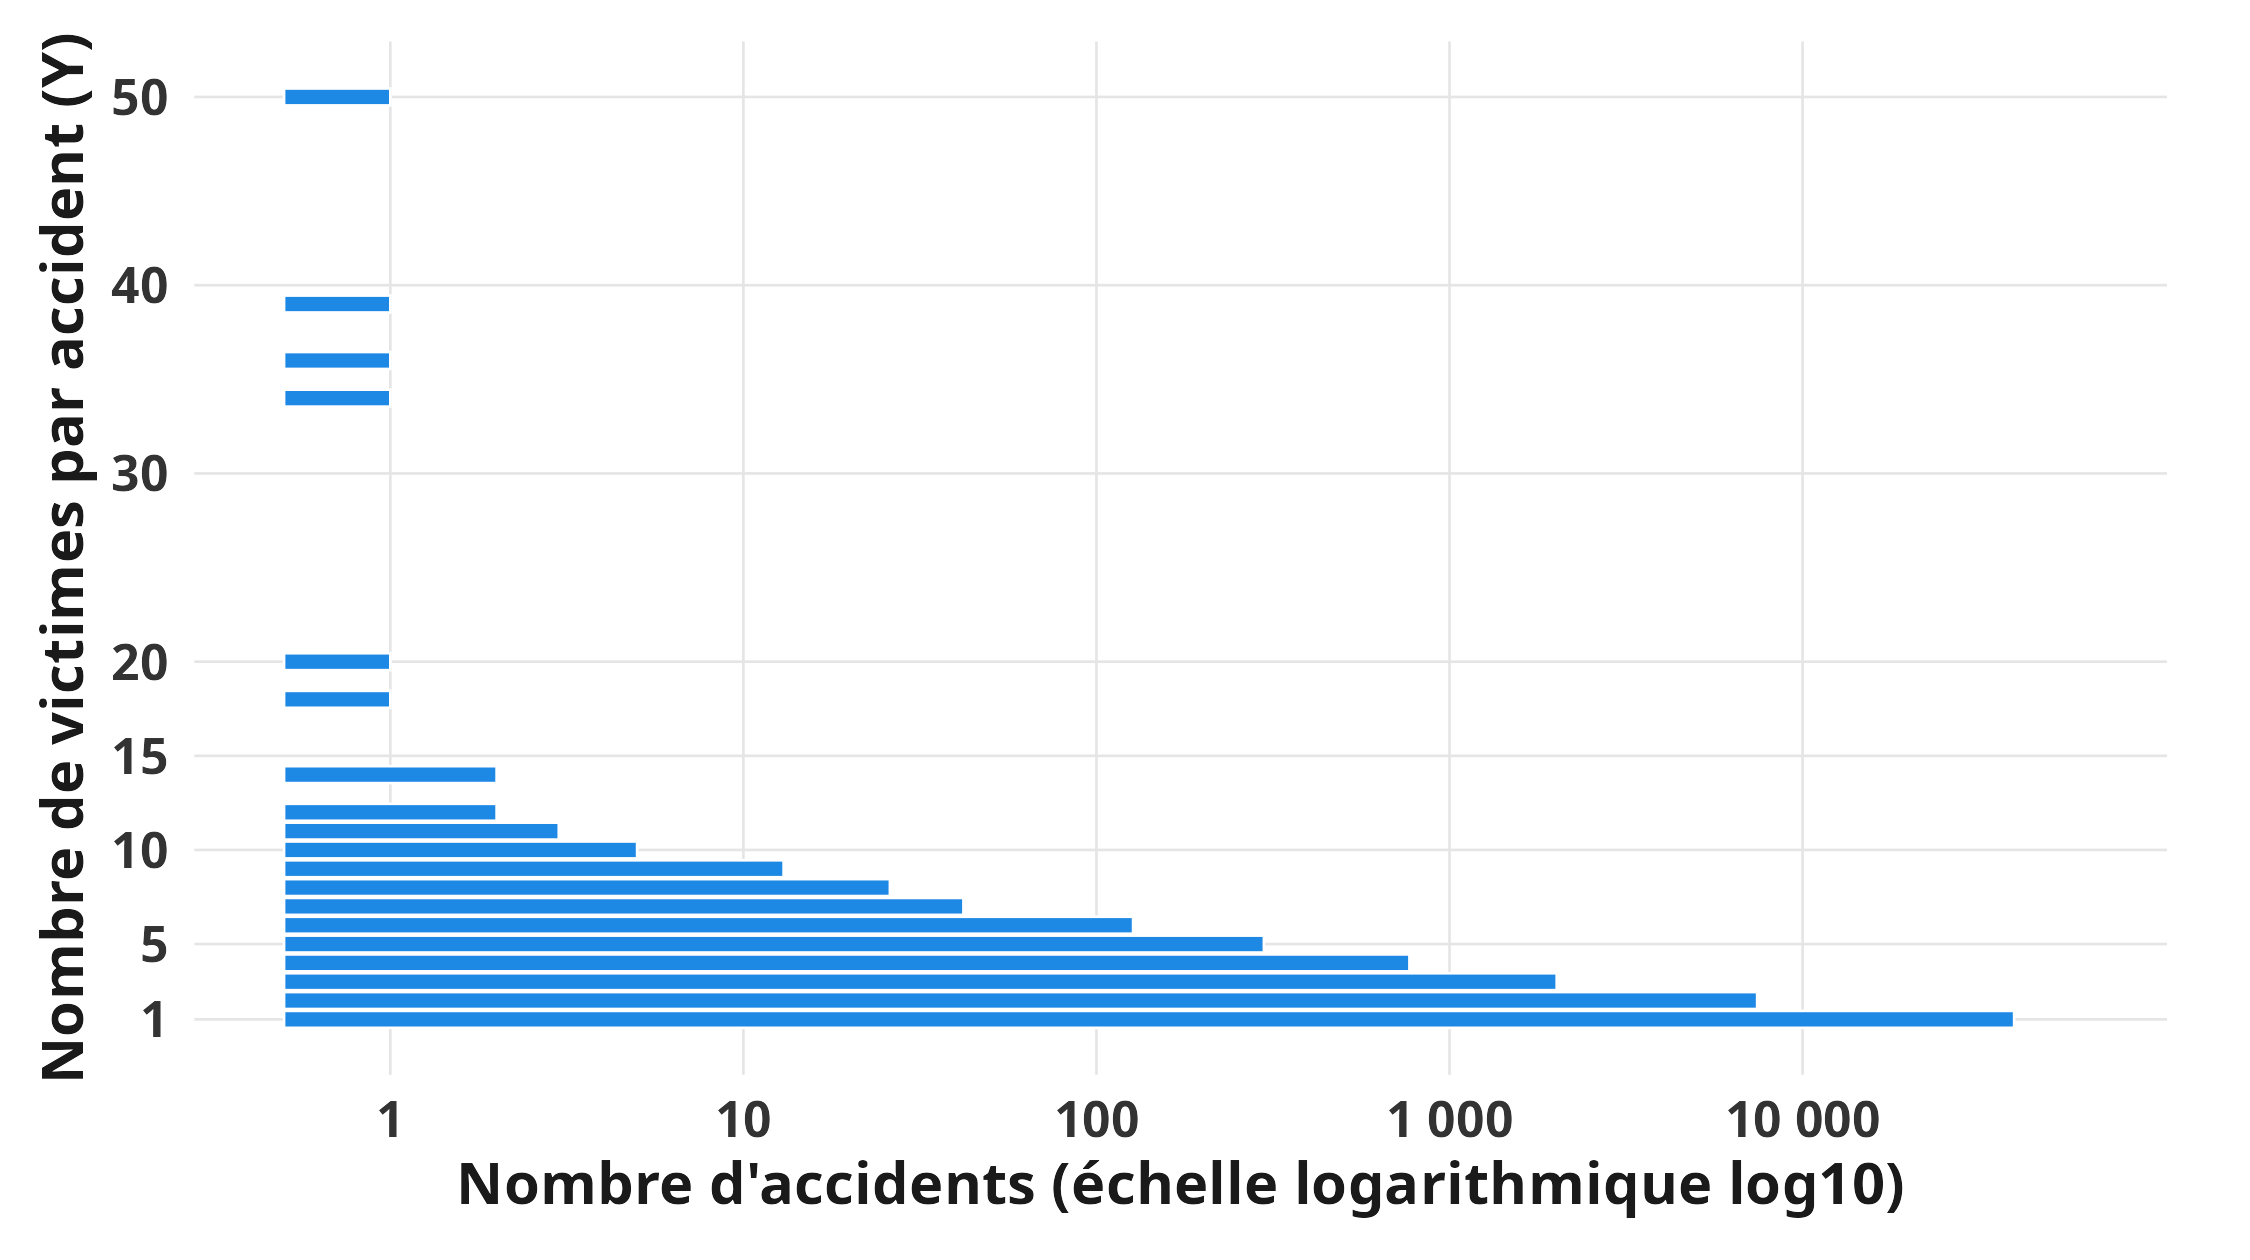
\includegraphics[width=0.75\linewidth]{g1_nb_victimes.png}
\caption{Distribution du nombre de victimes par accident corporel (échelle logarithmique sur l'axe des effectifs).}
\label{fig:dist_y}
\end{figure}

\noindent\textbf{Principales caractéristiques de la variable $Y$ :}
\begin{itemize}
    \item \textbf{Forte prédominance des accidents à 1 victime :} $78{,}72\,\%$ des accidents ne comptent qu'une seule victime corporelle ($n = 39\,744$). $14{,}73\,\%$ comptent 2 victimes ($n = 7\,436$), $3{,}99\,\%$ en comptent 3 ($n = 2\,012$), et $2{,}56\,\%$ en comptent 4 ou plus avec un maximum de 50 victimes, dans un accident impliquant un autocar.
    \item \textbf{Distribution asymétrique :} La médiane est égale à 1 et la moyenne à $1{,}33$, ce qui montre un étalement de la distribution vers la droite.
    \item \textbf{Non-normalité :} La variable étant discrète et fortement asymétrique, les tests gaussiens classiques (comme l'ANOVA) ne sont pas adaptés. Nous privilégierons donc des tests non paramétriques (Wilcoxon, Kruskal-Wallis).
\end{itemize}

\subsection{Variables temporelles : saisonnalité, mois, jour de la semaine et heure}

L'analyse de la temporalité des accidents corporels permet de distinguer plusieurs échelles de variations :
\begin{itemize}
    \item \textbf{Saisonnalité :} L'été concentre le volume maximal d'accidents ($27{,}26\,\%$, $n = 13\,762$), suivi de l'automne ($25{,}64\,\%$, $n = 12\,944$) et du printemps ($24{,}71\,\%$, $n = 12\,477$) ; l'hiver enregistre le volume le plus faible ($22{,}39\,\%$, $n = 11\,303$).
    \item \textbf{Évolution mensuelle :} La sinistralité culmine durant les mois estivaux (juillet avec $4\,868$ accidents et juin avec $4\,807$), tandis que février ($3\,498$) et janvier ($3\,747$) affichent les effectifs les plus réduits.
    \item \textbf{Rythme hebdomadaire :} Le vendredi enregistre le pic d'accidents ($8\,310$, soit $16{,}46\,\%$) en raison du cumul des trajets travail-domicile et des départs en week-end. Le dimanche compte le moins d'accidents ($6\,143$, soit $12{,}17\,\%$).
    \item \textbf{Rythme horaire :} La distribution horaire fait apparaître deux pics très nets aux heures de pointe pendulaires : à 8h ($2\,955$ accidents) et surtout entre 17h et 18h (respectivement $4\,531$ et $4\,573$ accidents), avec un creux nocturne marqué entre 3h et 5h du matin.
\end{itemize}

\begin{figure}[H]
\centering
\begin{minipage}[b]{0.48\linewidth}
    \centering
    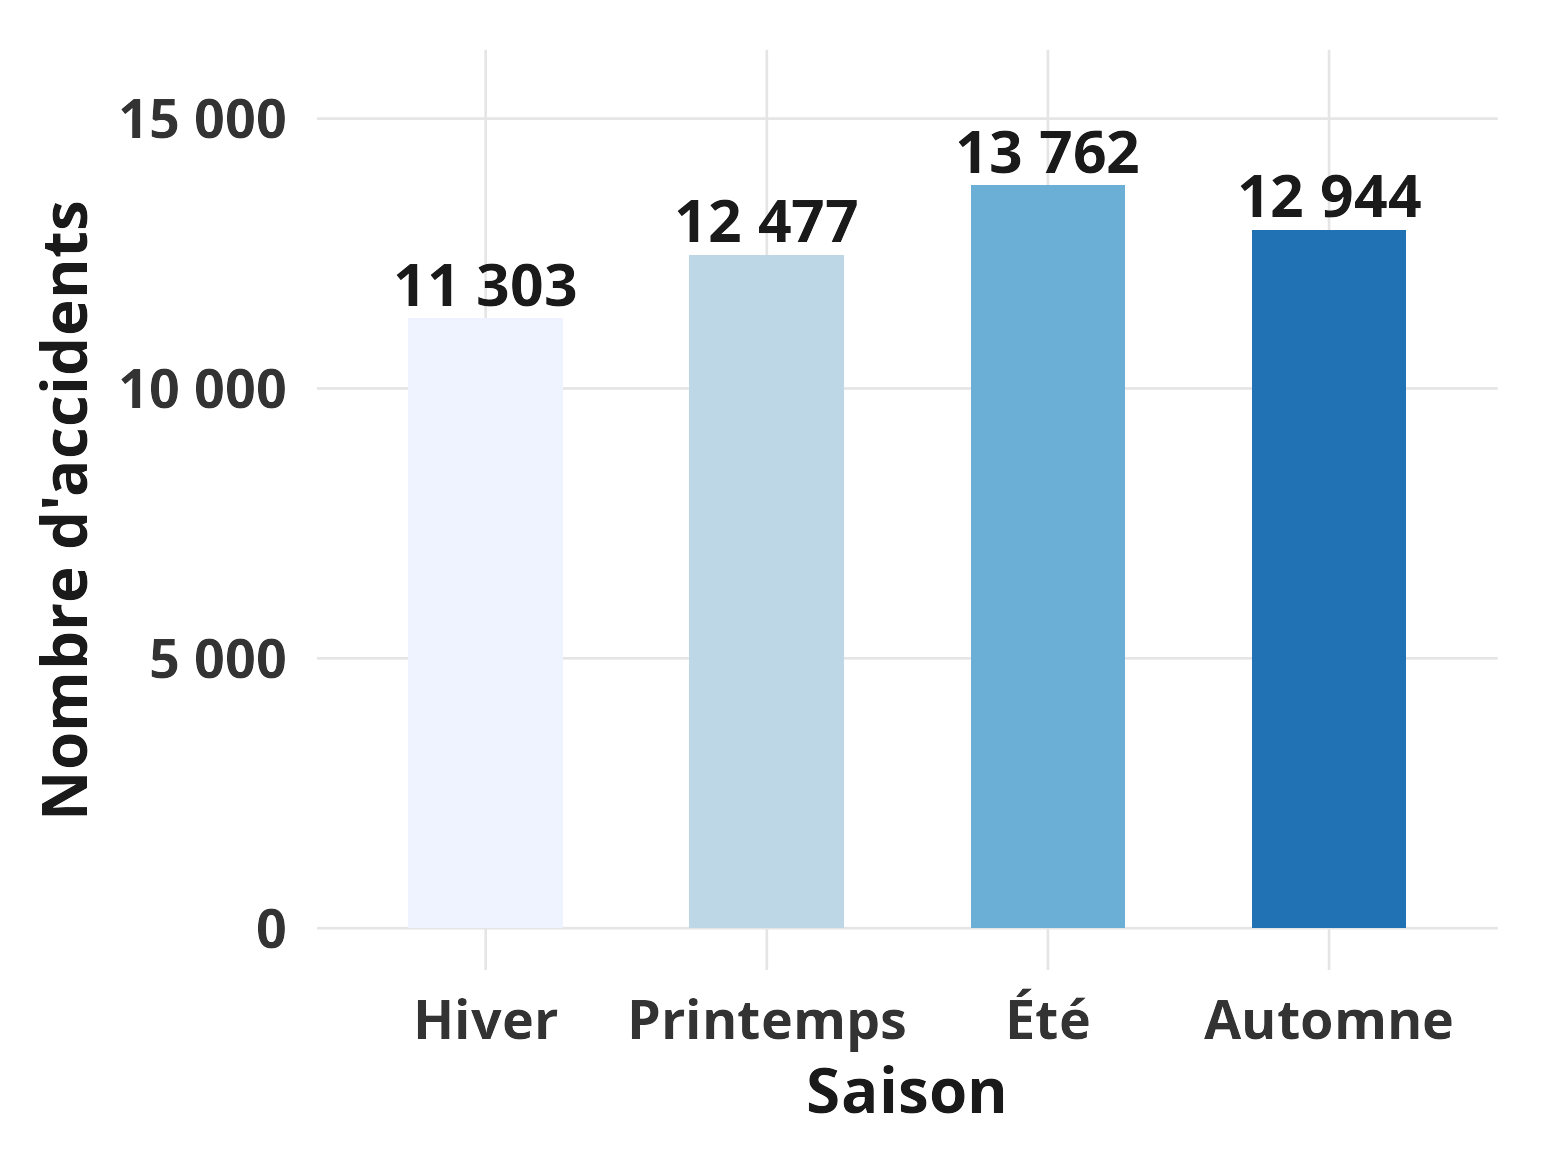
\includegraphics[width=\linewidth]{univ_saison.png}
    \caption{Distribution des accidents par saison.}
    \label{fig:univ_saison}
\end{minipage}
\hfill
\begin{minipage}[b]{0.48\linewidth}
    \centering
    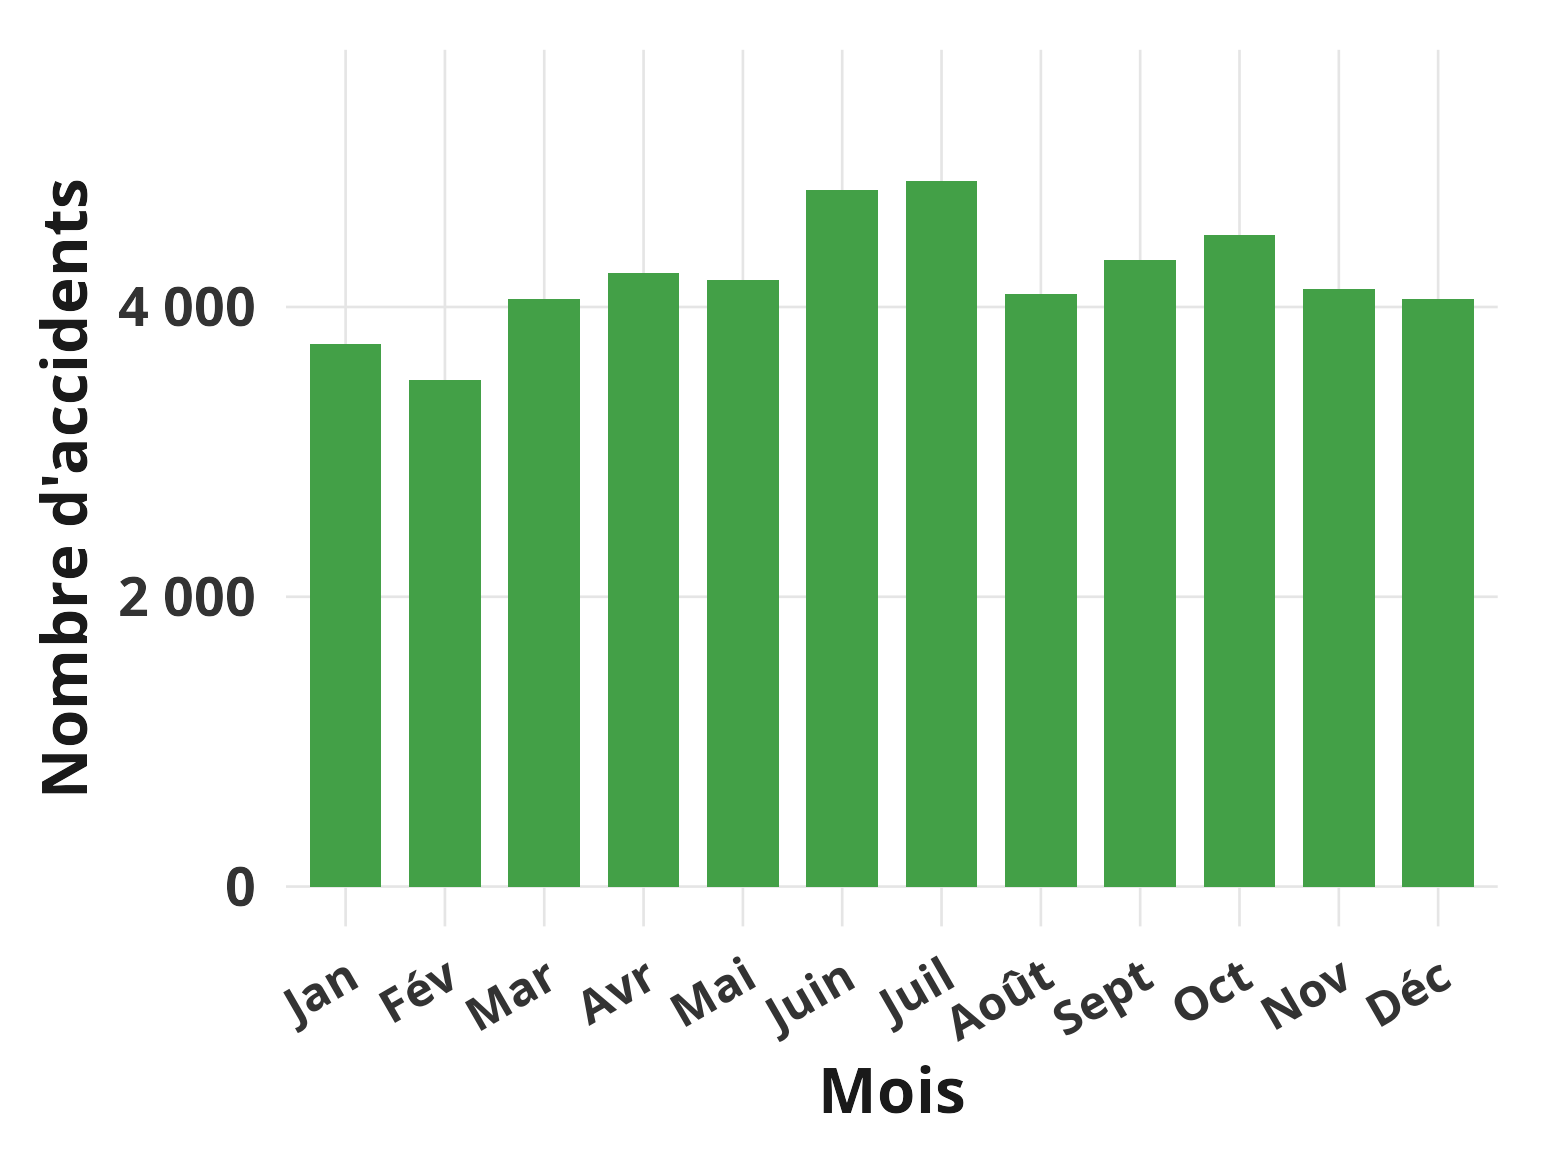
\includegraphics[width=\linewidth]{univ_mois.png}
    \caption{Distribution des accidents par mois (2024).}
    \label{fig:univ_mois}
\end{minipage}
\end{figure}

\begin{figure}[H]
\centering
\begin{minipage}[b]{0.48\linewidth}
    \centering
    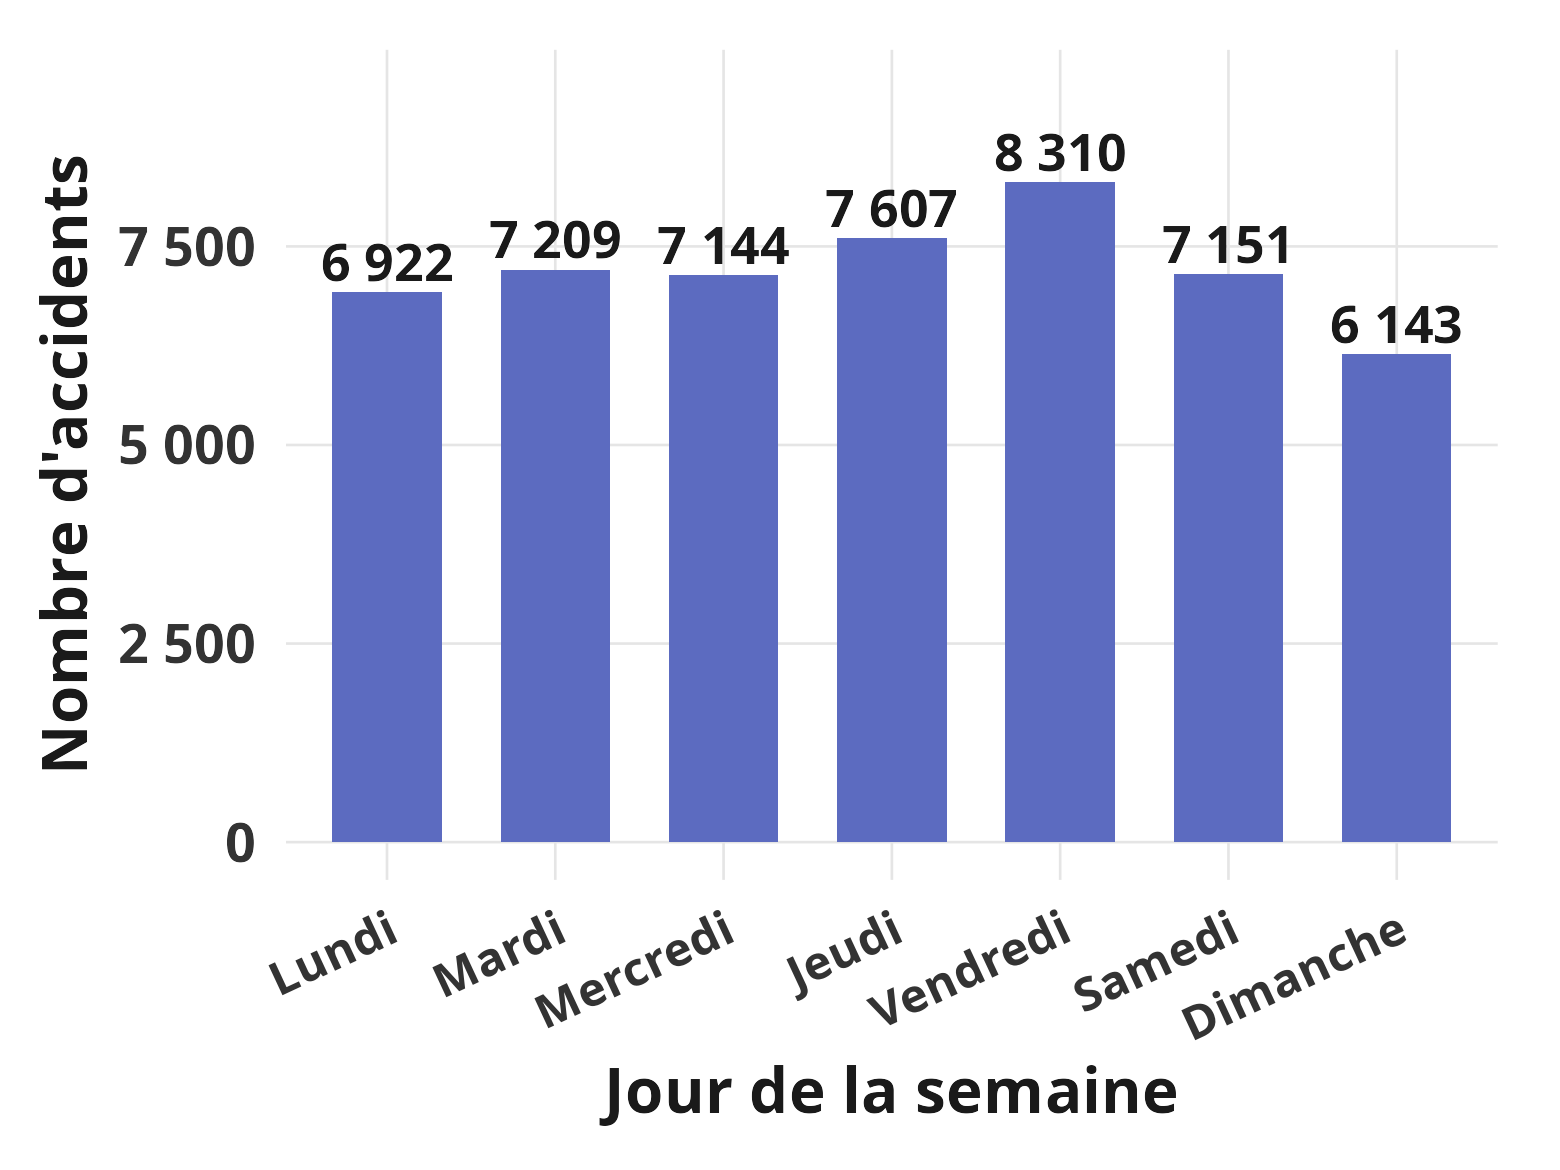
\includegraphics[width=\linewidth]{univ_jour.png}
    \caption{Distribution par jour de la semaine.}
    \label{fig:univ_jour}
\end{minipage}
\hfill
\begin{minipage}[b]{0.48\linewidth}
    \centering
    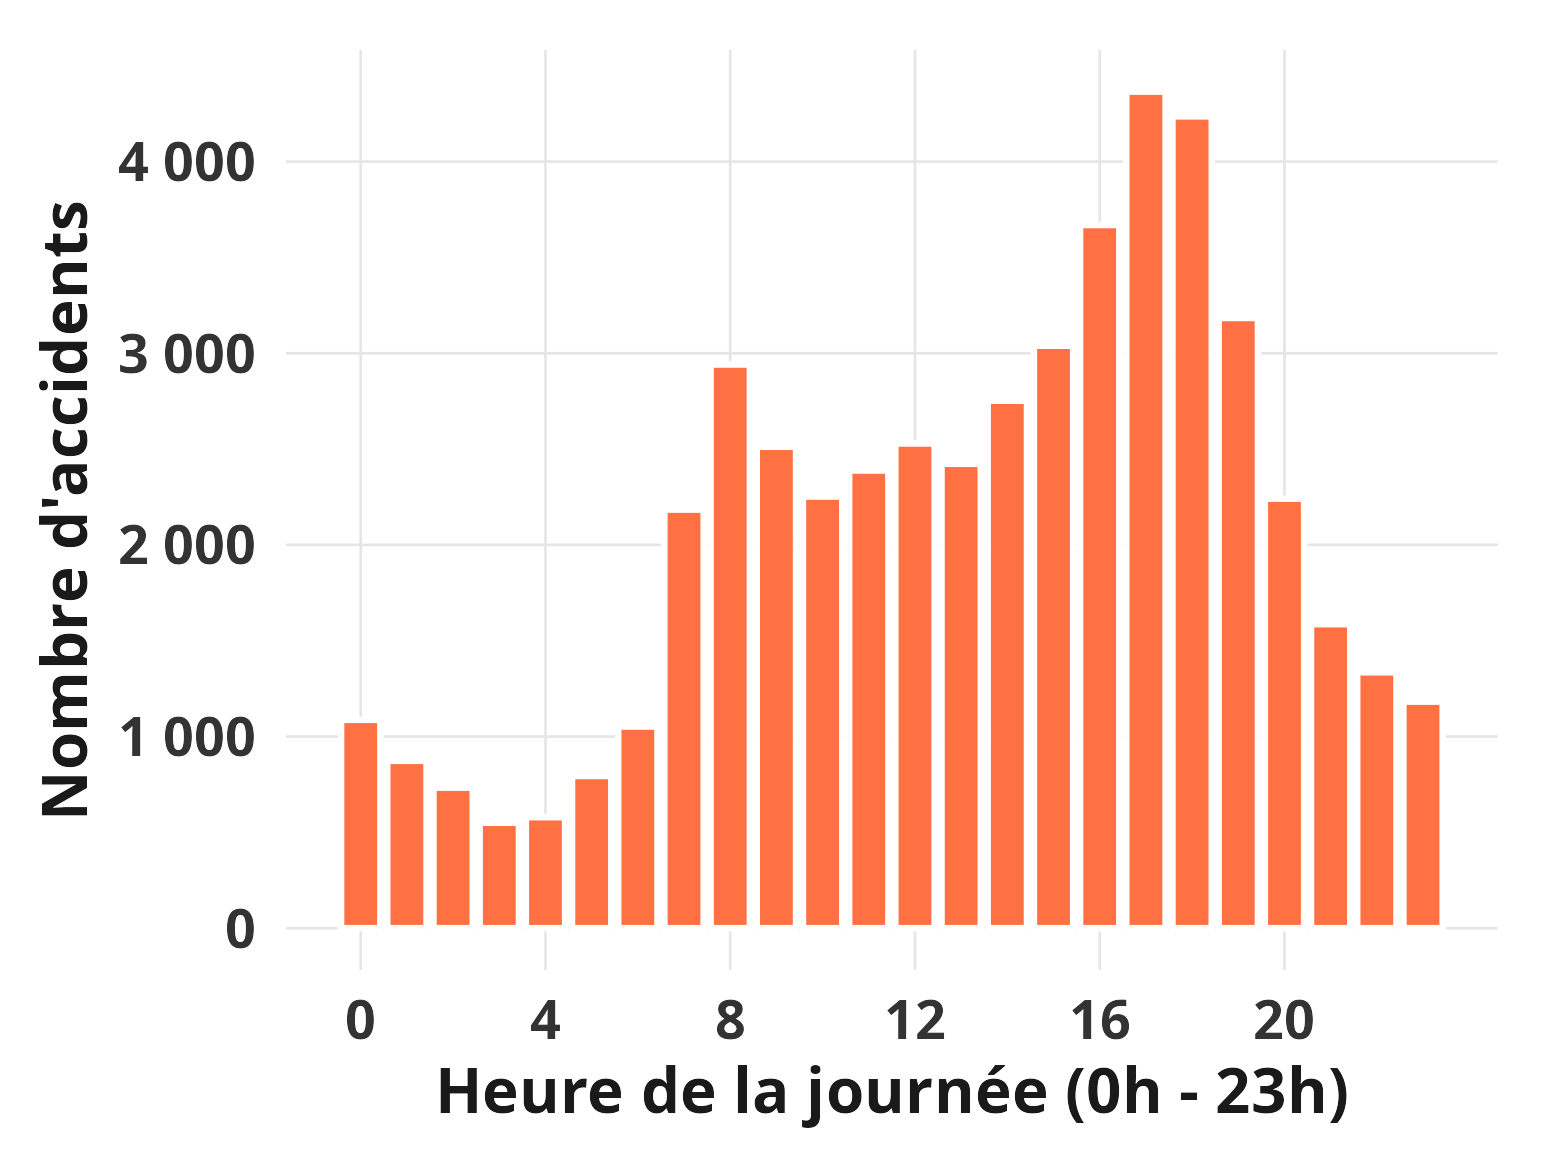
\includegraphics[width=\linewidth]{univ_heure.png}
    \caption{Distribution horaire (rythme circadien).}
    \label{fig:univ_heure}
\end{minipage}
\end{figure}

\subsection{Conditions environnementales : luminosité et météorologie}

Les conditions environnementales influencent fortement la visibilité et l'adhérence :
\begin{itemize}
    \item \textbf{Conditions de luminosité :} Près des deux tiers des accidents ($65{,}56\,\%$, $n = 33\,097$) ont lieu en plein jour. La nuit avec éclairage public allumé représente $15{,}51\,\%$ des cas ($n = 7\,829$), la nuit sans éclairage public en campagne $11{,}13\,\%$ ($n = 5\,617$), le crépuscule ou l'aube $6{,}69\,\%$ ($n = 3\,379$), et la nuit avec éclairage public non allumé $1{,}12\,\%$ ($n = 564$).
\end{itemize}

\begin{figure}[H]
\centering
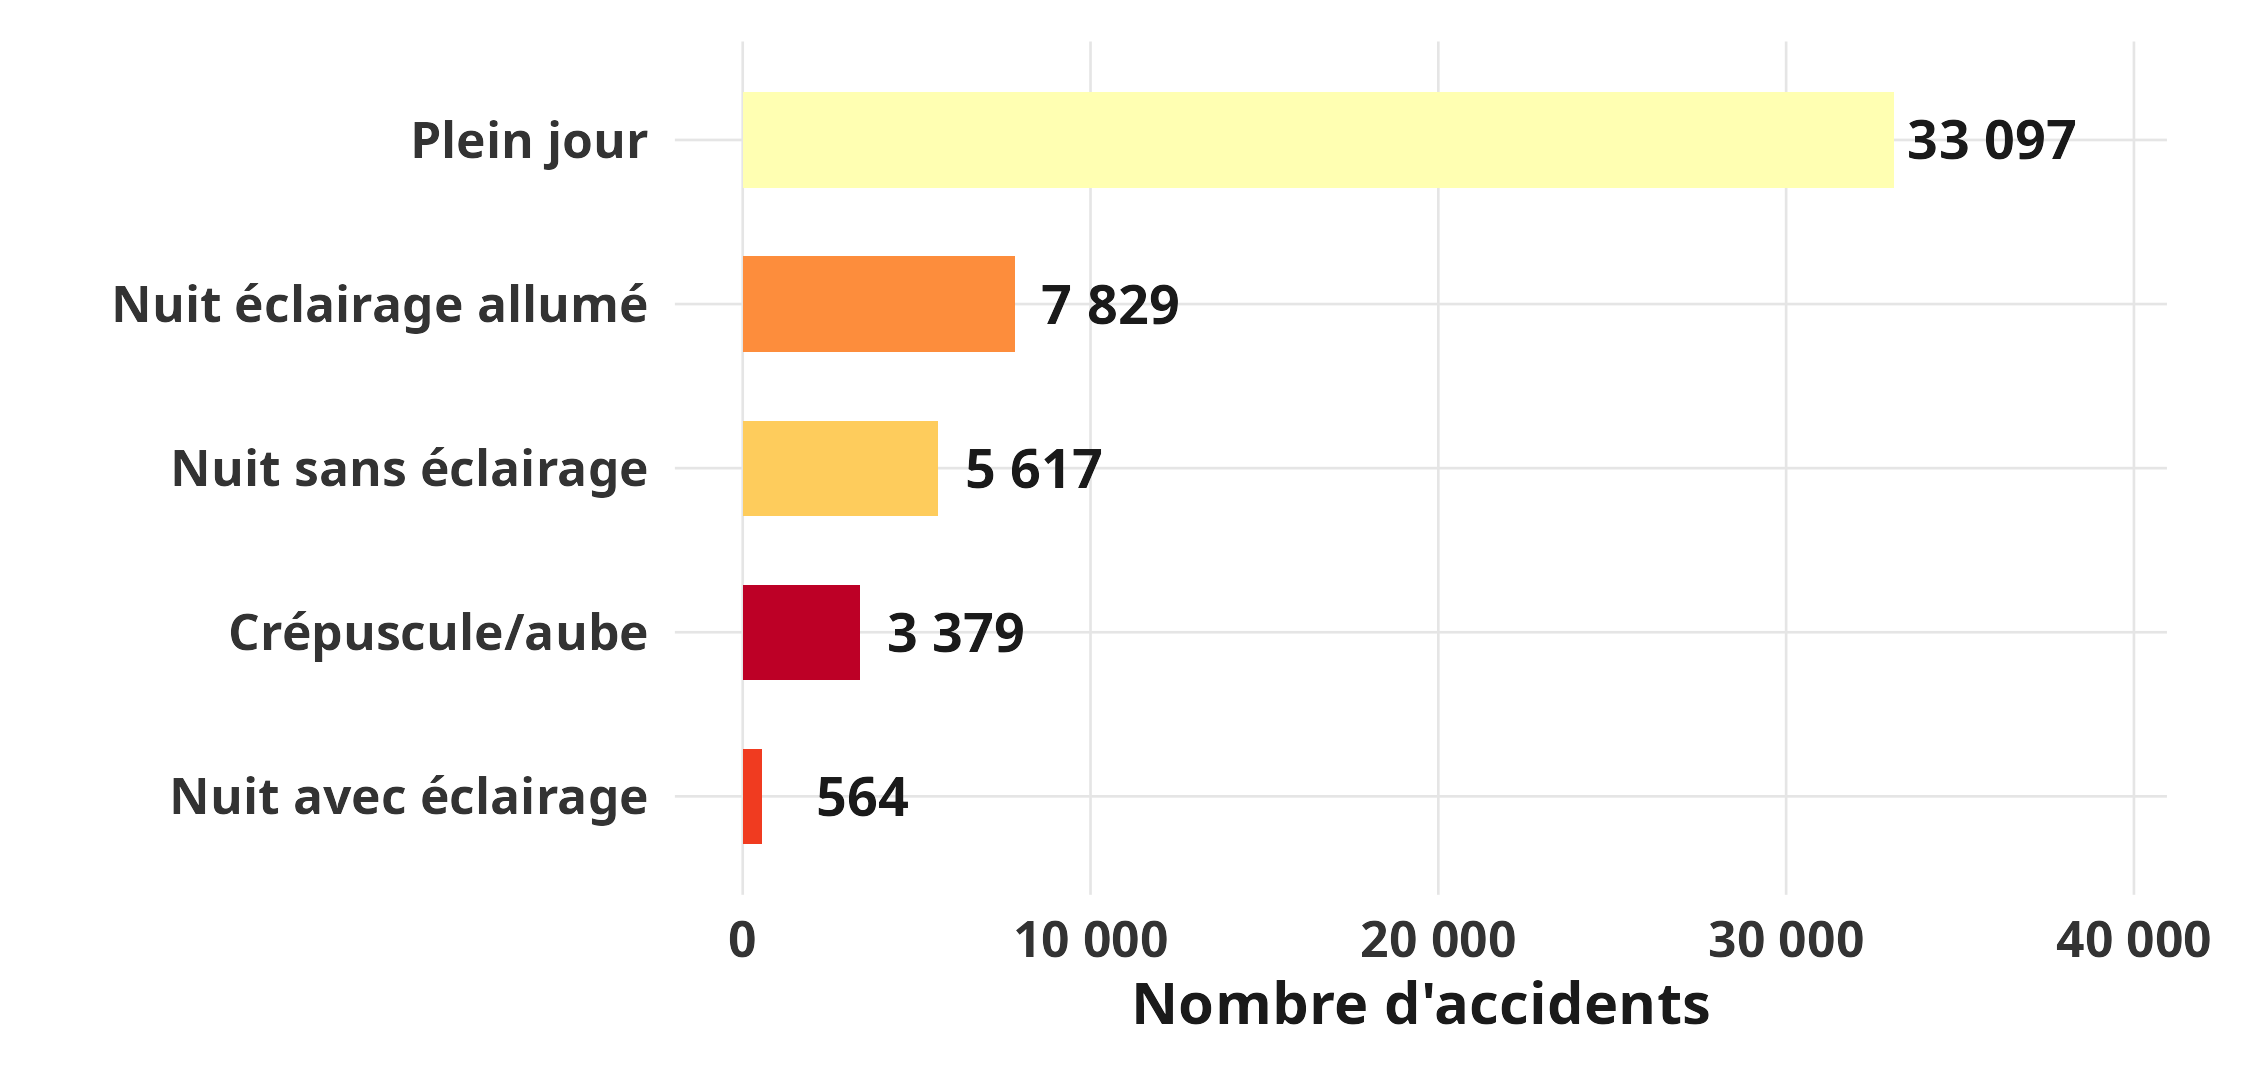
\includegraphics[width=0.75\linewidth]{univ_lum.png}
\caption{Distribution des accidents selon les conditions de luminosité.}
\label{fig:univ_lum}
\end{figure}
\begin{itemize}
    \item \textbf{Conditions météorologiques :} Une météo normale prédomine largement ($76{,}05\,\%$, $n = 38\,394$). La pluie est présente dans $15{,}50\,\%$ des cas ($12{,}80\,\%$ de pluie légère, $n = 6\,464$ ; $2{,}70\,\%$ de pluie forte, $n = 1\,364$). Les conditions extrêmes (brouillard $1{,}04\,\%$, neige ou grêle $0{,}46\,\%$, vent fort $0{,}33\,\%$) demeurent rares en volume absolu.
\end{itemize}

\begin{figure}[H]
\centering
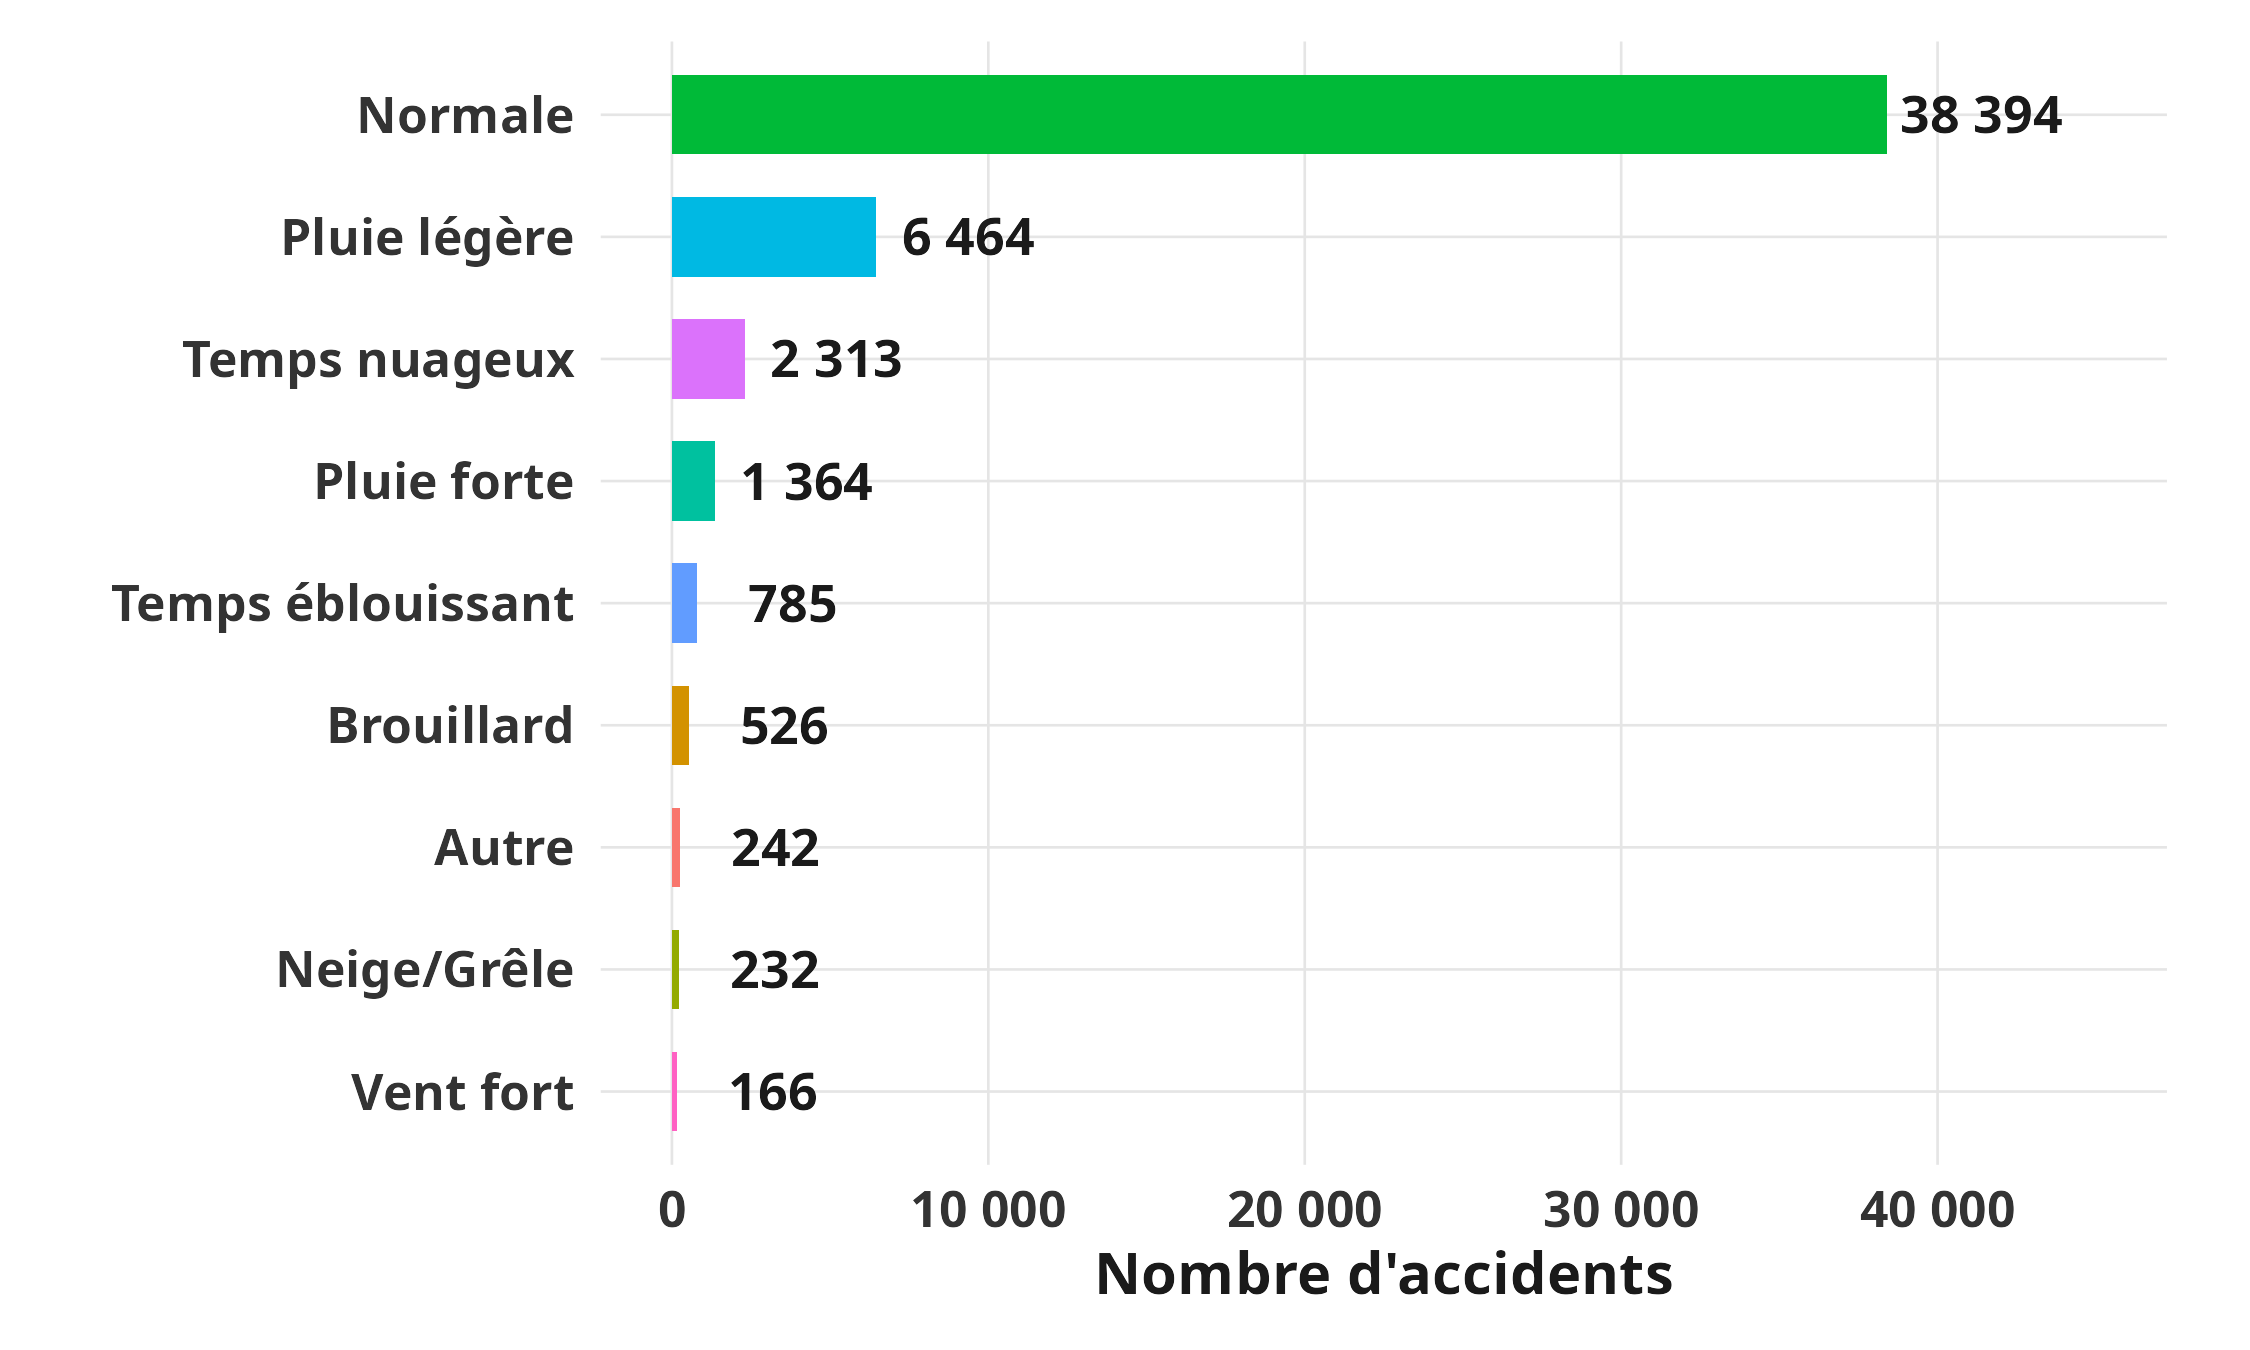
\includegraphics[width=0.78\linewidth]{univ_atm.png}
\caption{Distribution des accidents selon les conditions météorologiques.}
\label{fig:univ_atm}
\end{figure}

\subsection{Infrastructure et typologie des collisions}

La configuration de l'infrastructure et le type d'impact définissent le cadre matériel des sinistres :
\begin{itemize}
    \item \textbf{Zone de localisation :} $62{,}87\,\%$ des accidents surviennent en agglomération ($n = 31\,739$, vitesse moyenne autorisée de $45{,}7$\,km/h) contre $37{,}13\,\%$ hors agglomération ($n = 18\,747$, vitesse moyenne autorisée de $83{,}6$\,km/h).
    \item \textbf{Typologie de collision :} Les collisions à deux véhicules par l'arrière ou sur le côté sont majoritaires ($43{,}26\,\%$, $n = 21\,838$), suivies des autres collisions ($29{,}61\,\%$, $n = 14\,948$), des collisions frontales ($10{,}96\,\%$, $n = 5\,533$) et des accidents sans collision contre un tiers ($9{,}96\,\%$, $n = 5\,029$). Les collisions à trois véhicules ou plus représentent $6{,}21\,\%$ de l'ensemble.
    \item \textbf{Type d'intersection :} $62{,}89\,\%$ des accidents ont lieu hors intersection ($n = 31\,749$). Lorsqu'une intersection est impliquée, les carrefours en T ($12{,}09\,\%$) et en X ($12{,}06\,\%$) précèdent les ronds-points ($5{,}02\,\%$) et les autres configurations.
\end{itemize}

\begin{figure}[H]
\centering
\begin{minipage}[b]{0.45\linewidth}
    \centering
    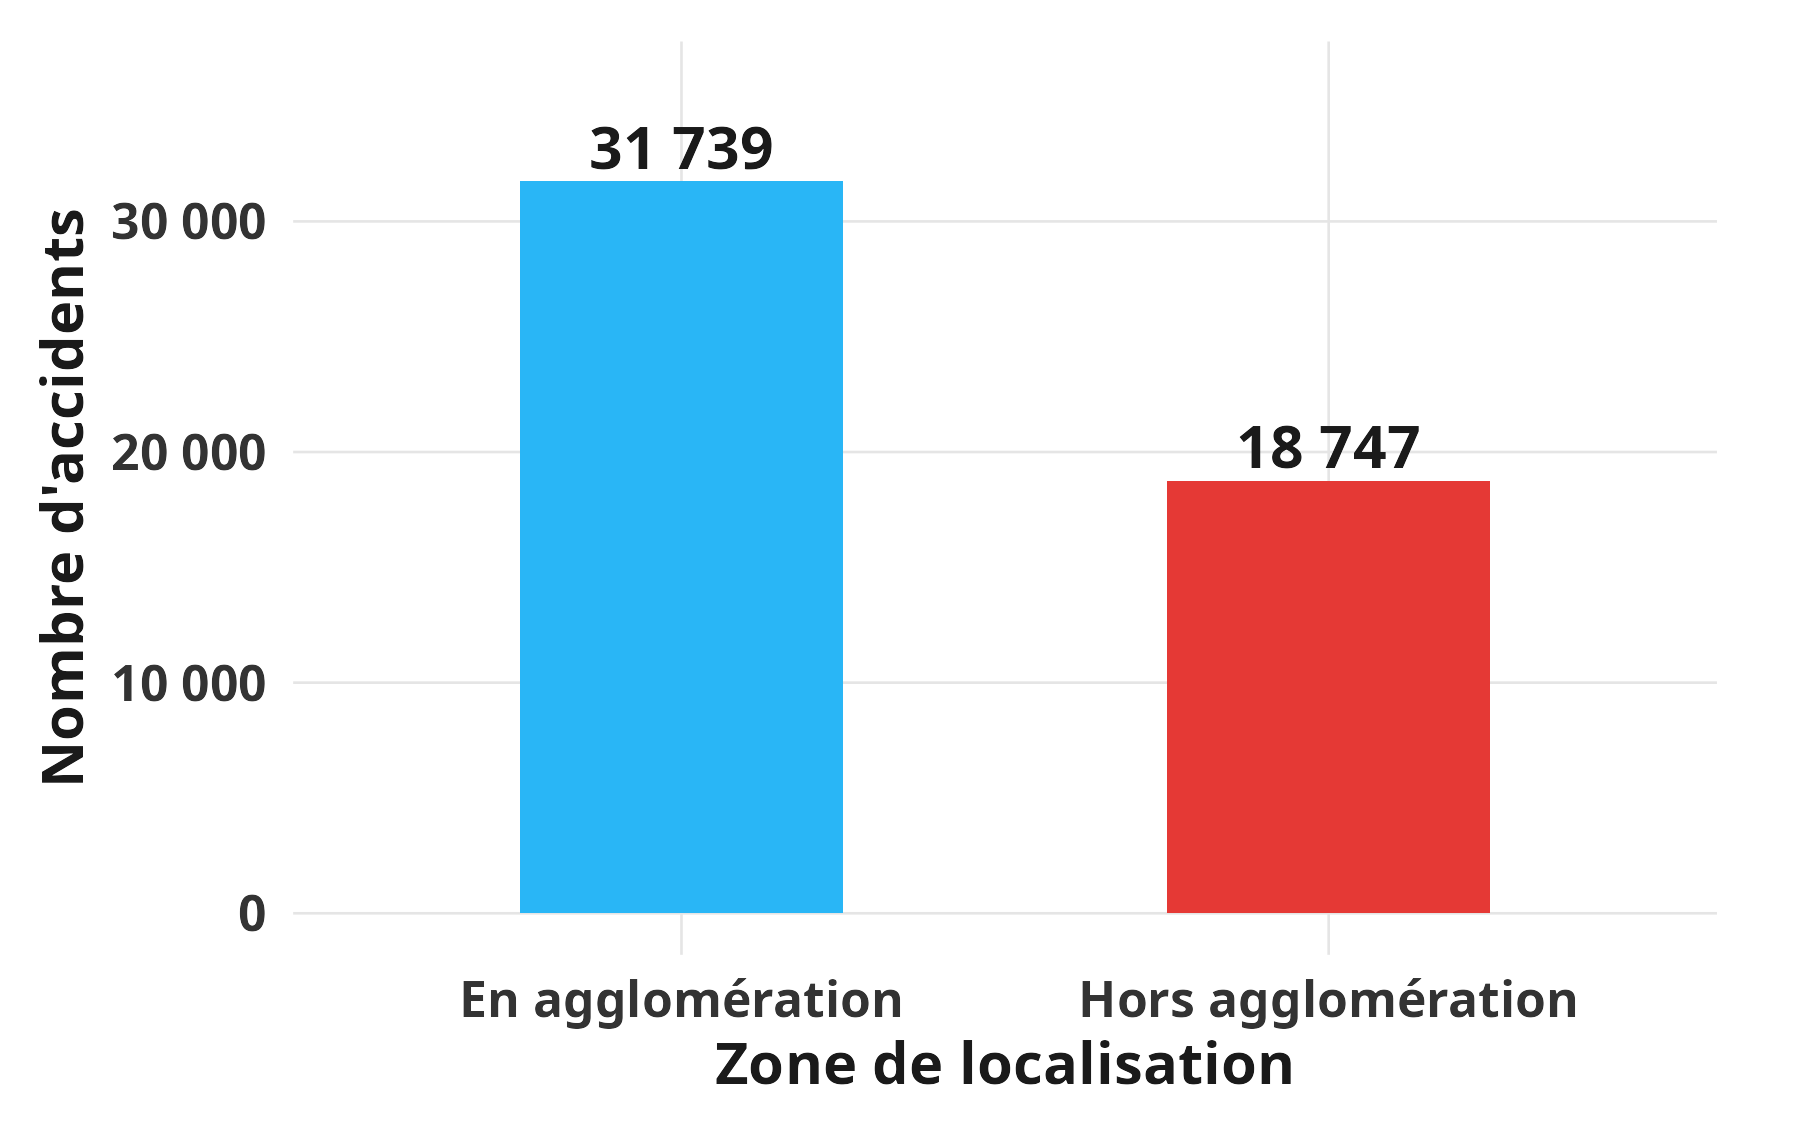
\includegraphics[width=\linewidth]{univ_agg.png}
    \caption{Répartition agglomération vs rurale.}
    \label{fig:univ_agg}
\end{minipage}
\hfill
\begin{minipage}[b]{0.51\linewidth}
    \centering
    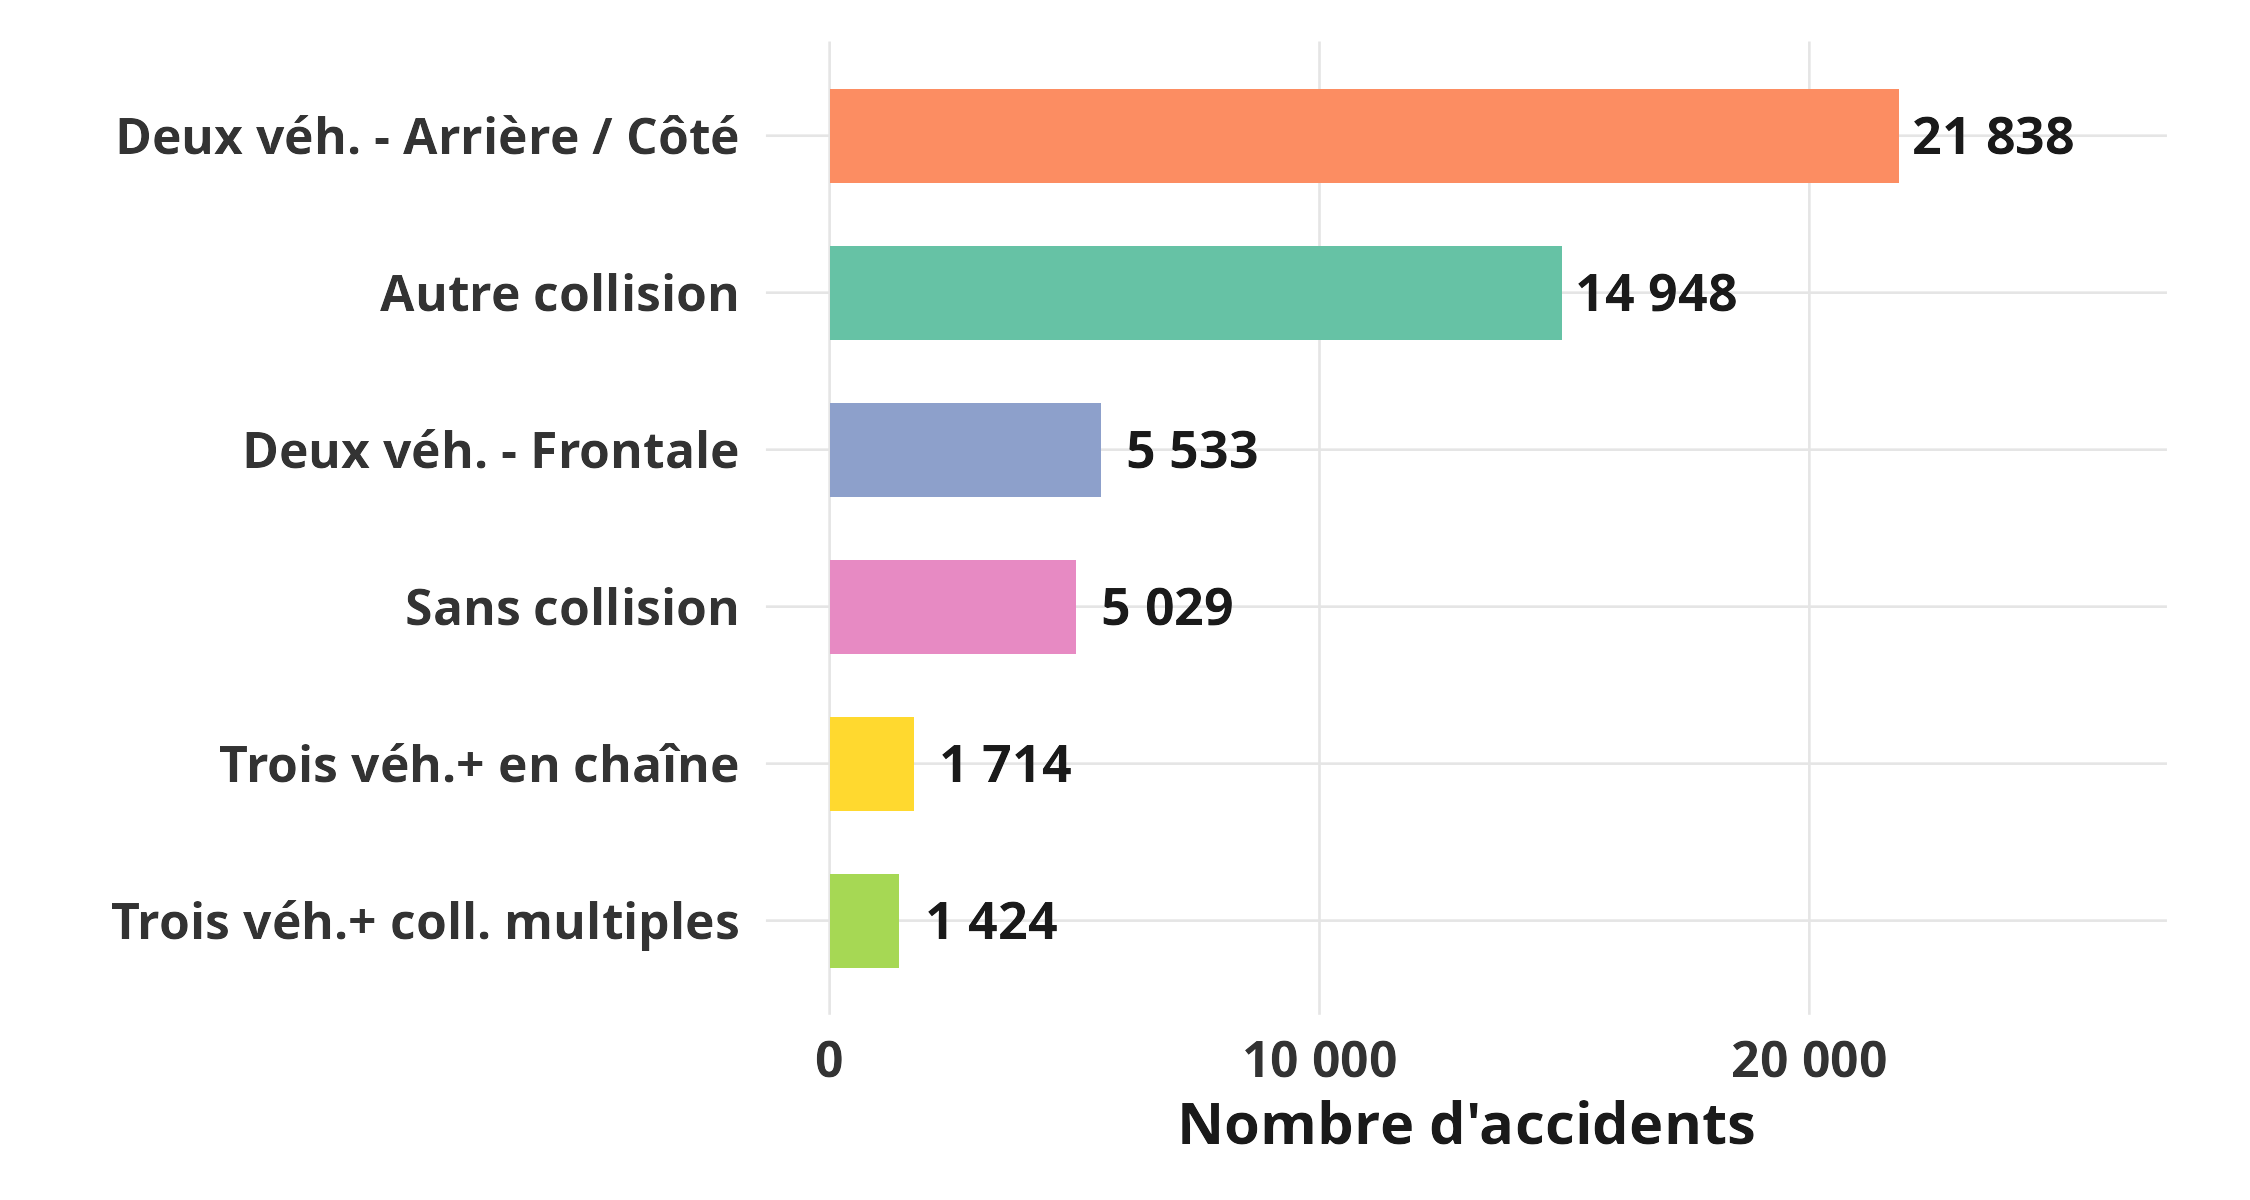
\includegraphics[width=\linewidth]{univ_col.png}
    \caption{Typologie de collision (6 catégories).}
    \label{fig:univ_col}
\end{minipage}
\end{figure}

\begin{figure}[H]
\centering
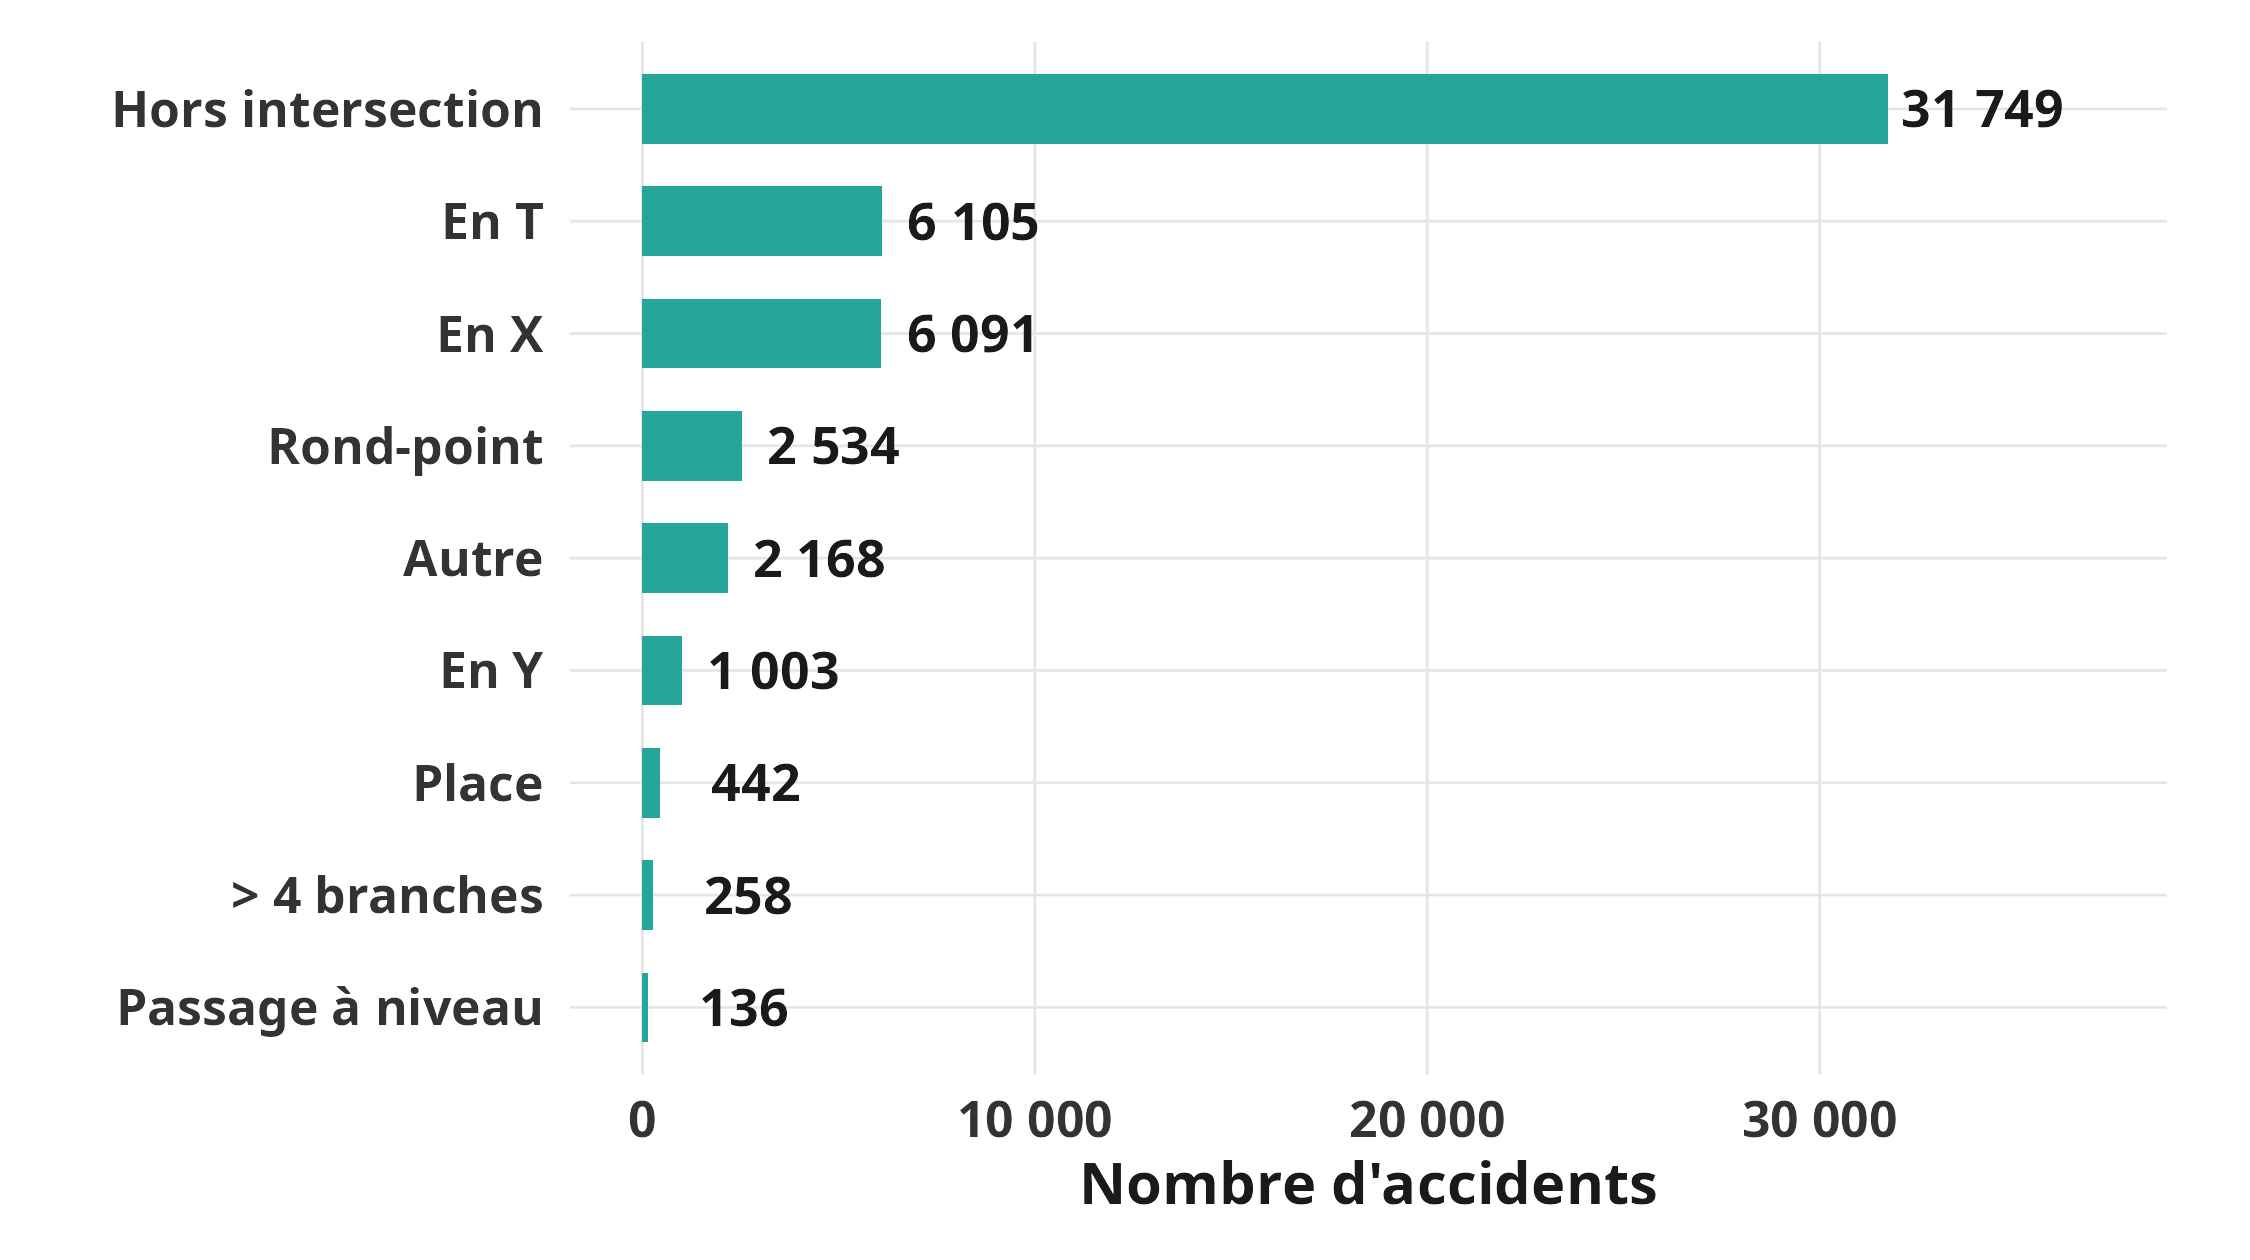
\includegraphics[width=0.78\linewidth]{univ_int.png}
\caption{Distribution des accidents selon la configuration de l'infrastructure (intersections).}
\label{fig:univ_int}
\end{figure}

\subsection{Standardisation géographique : Taux pour 100 000 habitants}
Regarder uniquement le total des accidents n'aurait pas grand sens : les départements les plus habités arriveraient forcément premiers. Pour faire une vraie comparaison, on rapporte le nombre d'accidents à la population de chaque département (pour $100,000$ habitants). Et en normalisant par la population légale municipale INSEE 2024 :
\[
\text{Taux départemental} = \frac{\text{Nombre d'accidents du département}}{\text{Population légale INSEE}} \times 100\,000
\]
En regardant les départements les plus touchés (Figure~\ref{fig:univ_top_dep}), on distingue clairement deux réalités : d'une part, l'Île-de-France, où la circulation est dense et permanente (Paris à $196{,}5$ accidents, Seine-Saint-Denis à $158{,}2$), et d'autre part, des zones rurales ou montagneuses, qui ont peu d'habitants mais voient passer beaucoup de touristes et de véhicules en transit (Pyrénées-Atlantiques $127{,}0$, Hautes-Alpes $121{,}3$, Cantal $120{,}6$).

\begin{figure}[H]
\centering
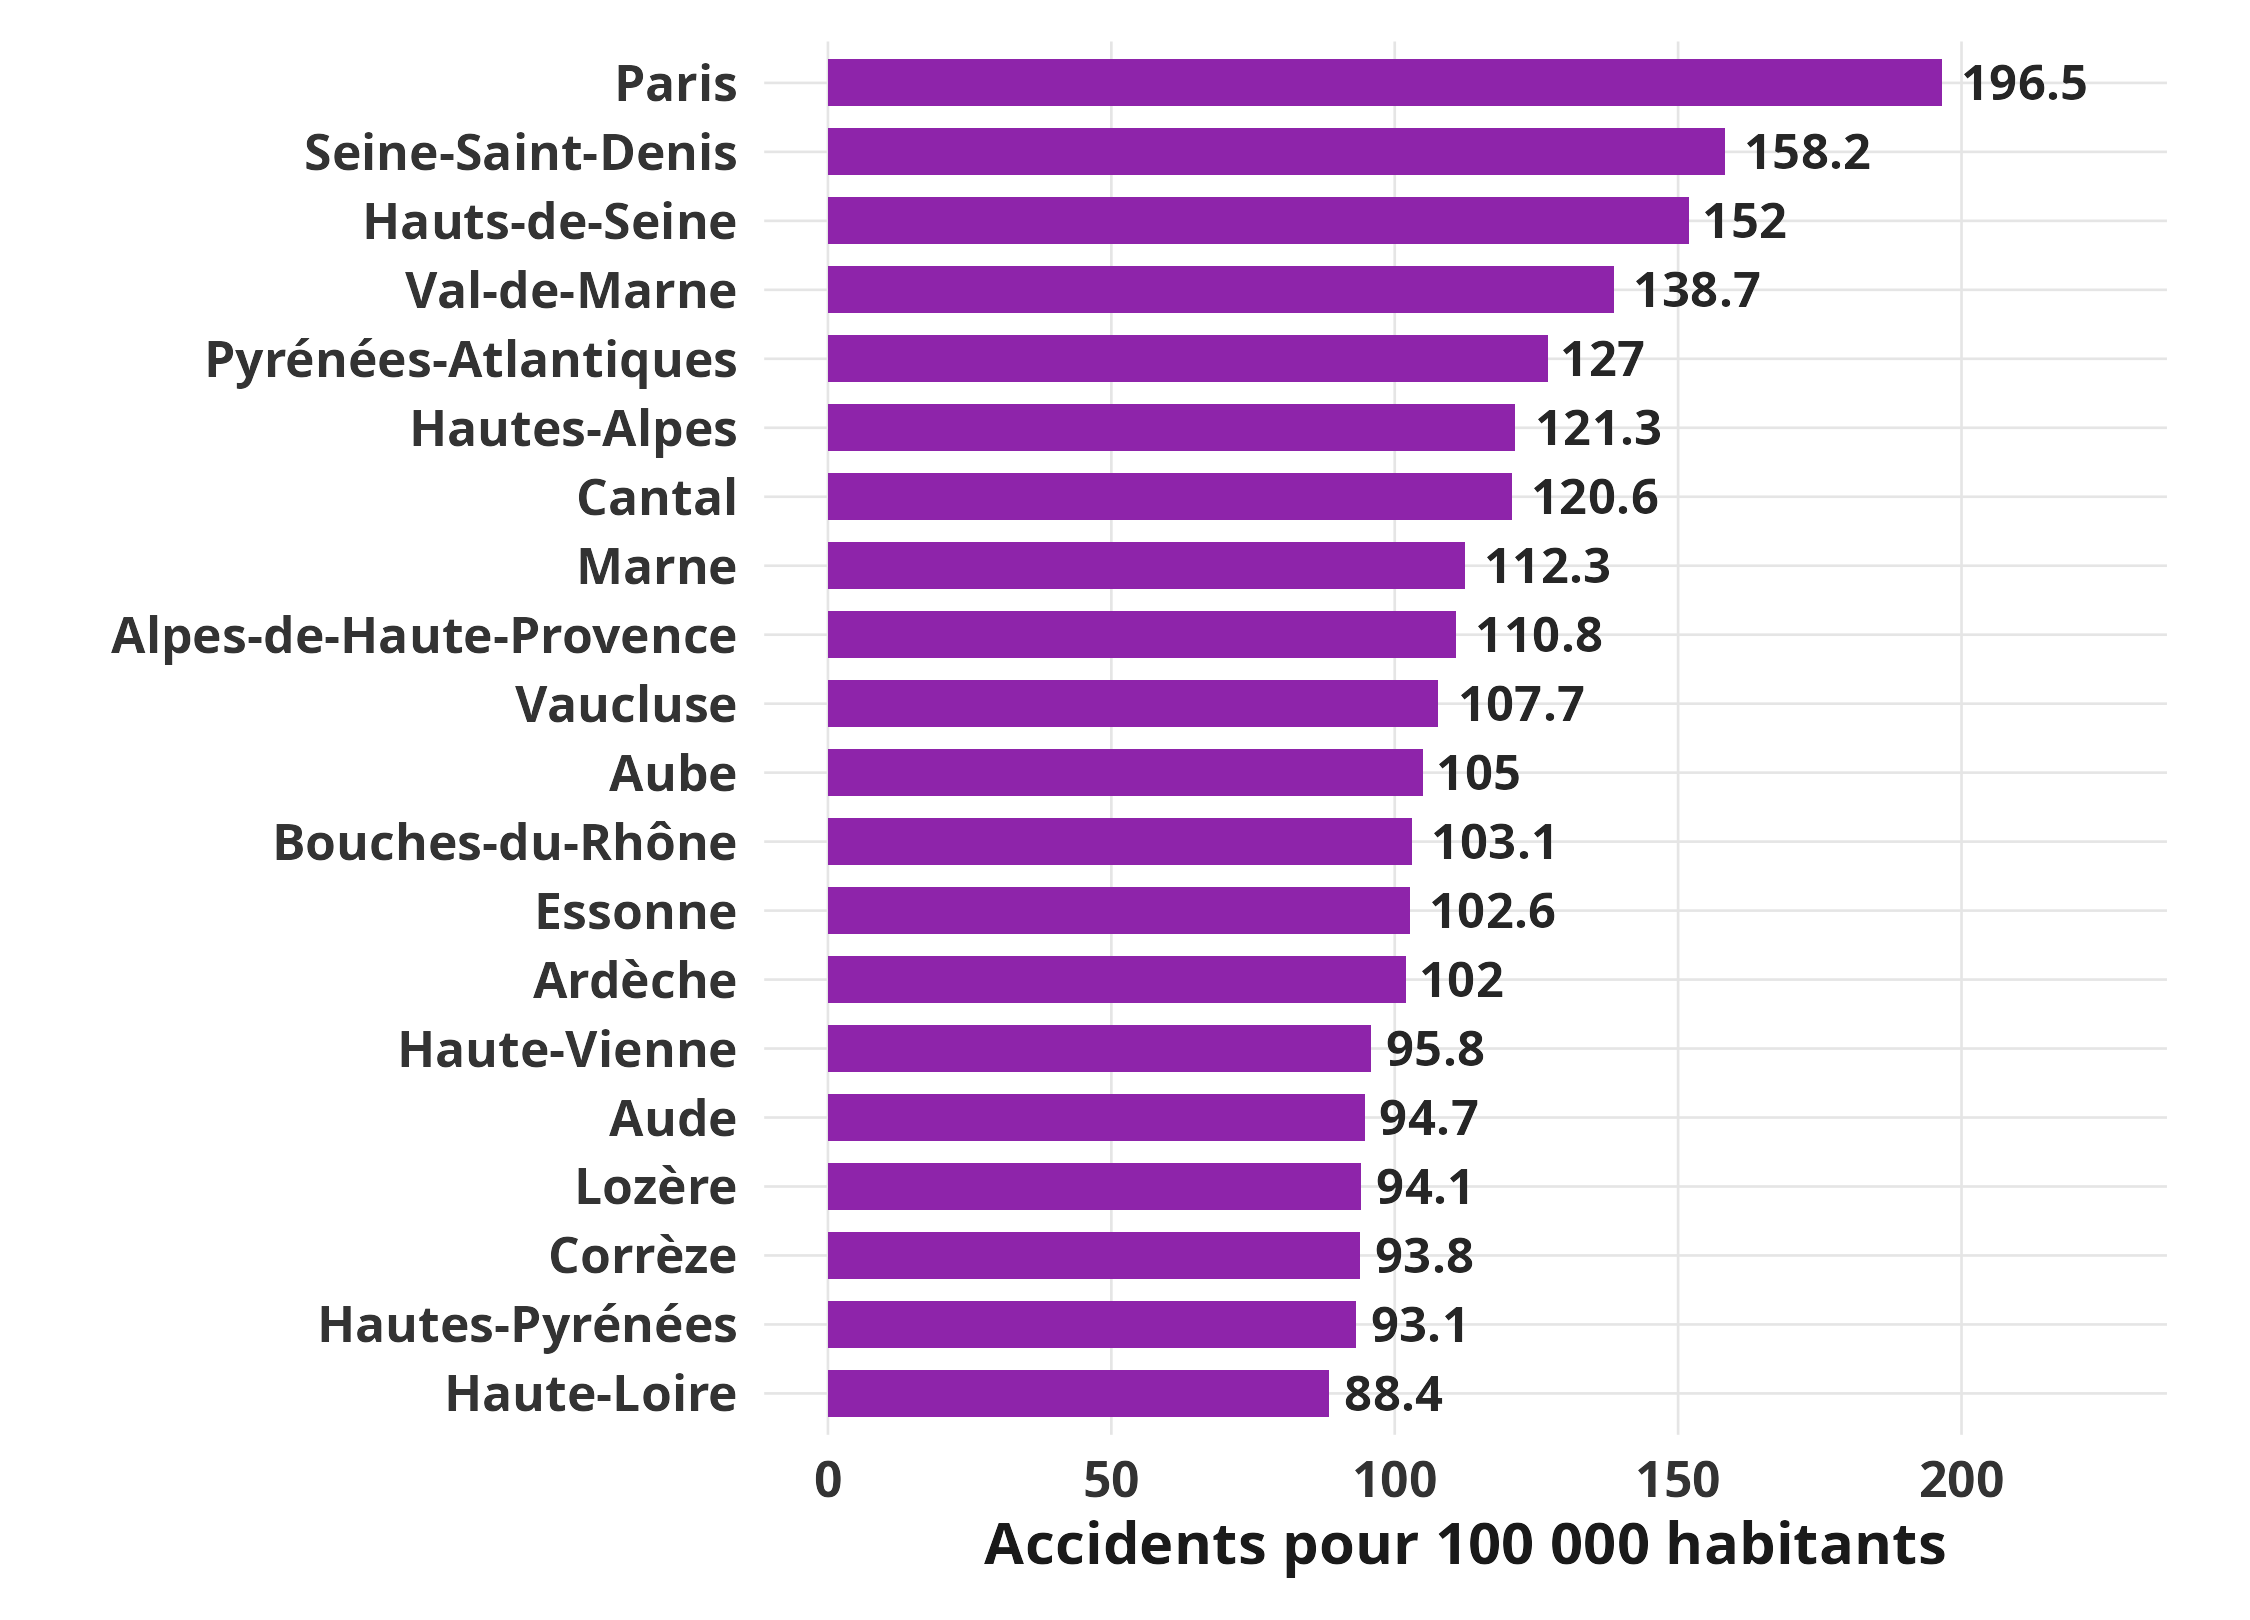
\includegraphics[width=0.75\linewidth]{univ_top_dep.png}
\caption{Top 20 des départements continentaux les plus accidentogènes selon le taux pour $100\,000$ habitants (INSEE 2024).}
\label{fig:univ_top_dep}
\end{figure}


% ==============================================================================
% SECTION 3 : ANALYSE BIVARIÉE ET TESTS D'HYPOTHÈSES FORMELS
% ==============================================================================
\section{Analyse Bivariée et Tests d'Hypothèses Formels}

L'analyse bivariée est organisée selon la nature des variables croisées. Pour la liaison entre une variable qualitative (ou une indicatrice) et le nombre de victimes, $Y$ n'est pas normale (section~2.1 ; test de Kolmogorov--Smirnov dans chaque saison) : toutes les comparaisons reposent donc sur des tests de rangs, Kruskal--Wallis (plus de deux groupes) ou Wilcoxon--Mann--Whitney (deux groupes). Pour la saison, la météo, la luminosité et la zone, ils sont complétés par un test d'égalité des variances (Bartlett ou Fisher) et, pour la saison, la météo et la zone, par un test de Welch qui ne suppose pas cette égalité. Les liaisons entre variables qualitatives sont étudiées par le test du $\chi^2$ et le V de Cramer, et les liaisons entre variables quantitatives par les corrélations de Pearson et de Spearman. L'hypothèse nulle est l'égalité des variances pour les tests de Bartlett et de Fisher, l'égalité des distributions pour les tests de Kruskal--Wallis et de Wilcoxon--Mann--Whitney, et l'égalité des moyennes pour les tests de Welch. Pour l'ensemble des tests statistiques menés dans cette étude, le seuil de significativité est fixé à $\alpha = 5\,\%$ ($0{,}05$) : toute $p$-valeur inférieure à ce seuil conduit au rejet de l'hypothèse nulle $H_0$.

\subsection{Facteurs explicatifs vs Nombre de victimes ($Y = \text{\texttt{Nb\_victimes}}$)}

\subsubsection{Saisonnalité ($Y \sim \text{\texttt{saison}}$)}
\begin{table}[H]
\centering
\small
\begin{tabular}{lccccc}
\toprule
\textbf{Saison} & \textbf{Effectif ($n_k$)} & \textbf{Moyenne} & \textbf{Médiane} & \textbf{Écart-type} & \textbf{Test de Normalité (K-S)} \\
\midrule
Hiver      & $11\,303$ & $1{,}325$ & 1 & $0{,}896$ & $D = 0{,}431$ ($p < 2{,}2 \times 10^{-16}$) \\
Printemps  & $12\,477$ & $1{,}313$ & 1 & $0{,}816$ & $D = 0{,}442$ ($p < 2{,}2 \times 10^{-16}$) \\
Été        & $13\,762$ & $\mathbf{1{,}349}$ & 1 & $0{,}835$ & $D = 0{,}437$ ($p < 2{,}2 \times 10^{-16}$) \\
Automne    & $12\,944$ & $1{,}314$ & 1 & $0{,}867$ & $D = 0{,}435$ ($p < 2{,}2 \times 10^{-16}$) \\
\bottomrule
\end{tabular}
\caption{Indicateurs du nombre de victimes par saison et tests de normalité ($n = 50\,486$).}
\label{tab:biv_saison}
\end{table}


\begin{figure}[H]
\centering
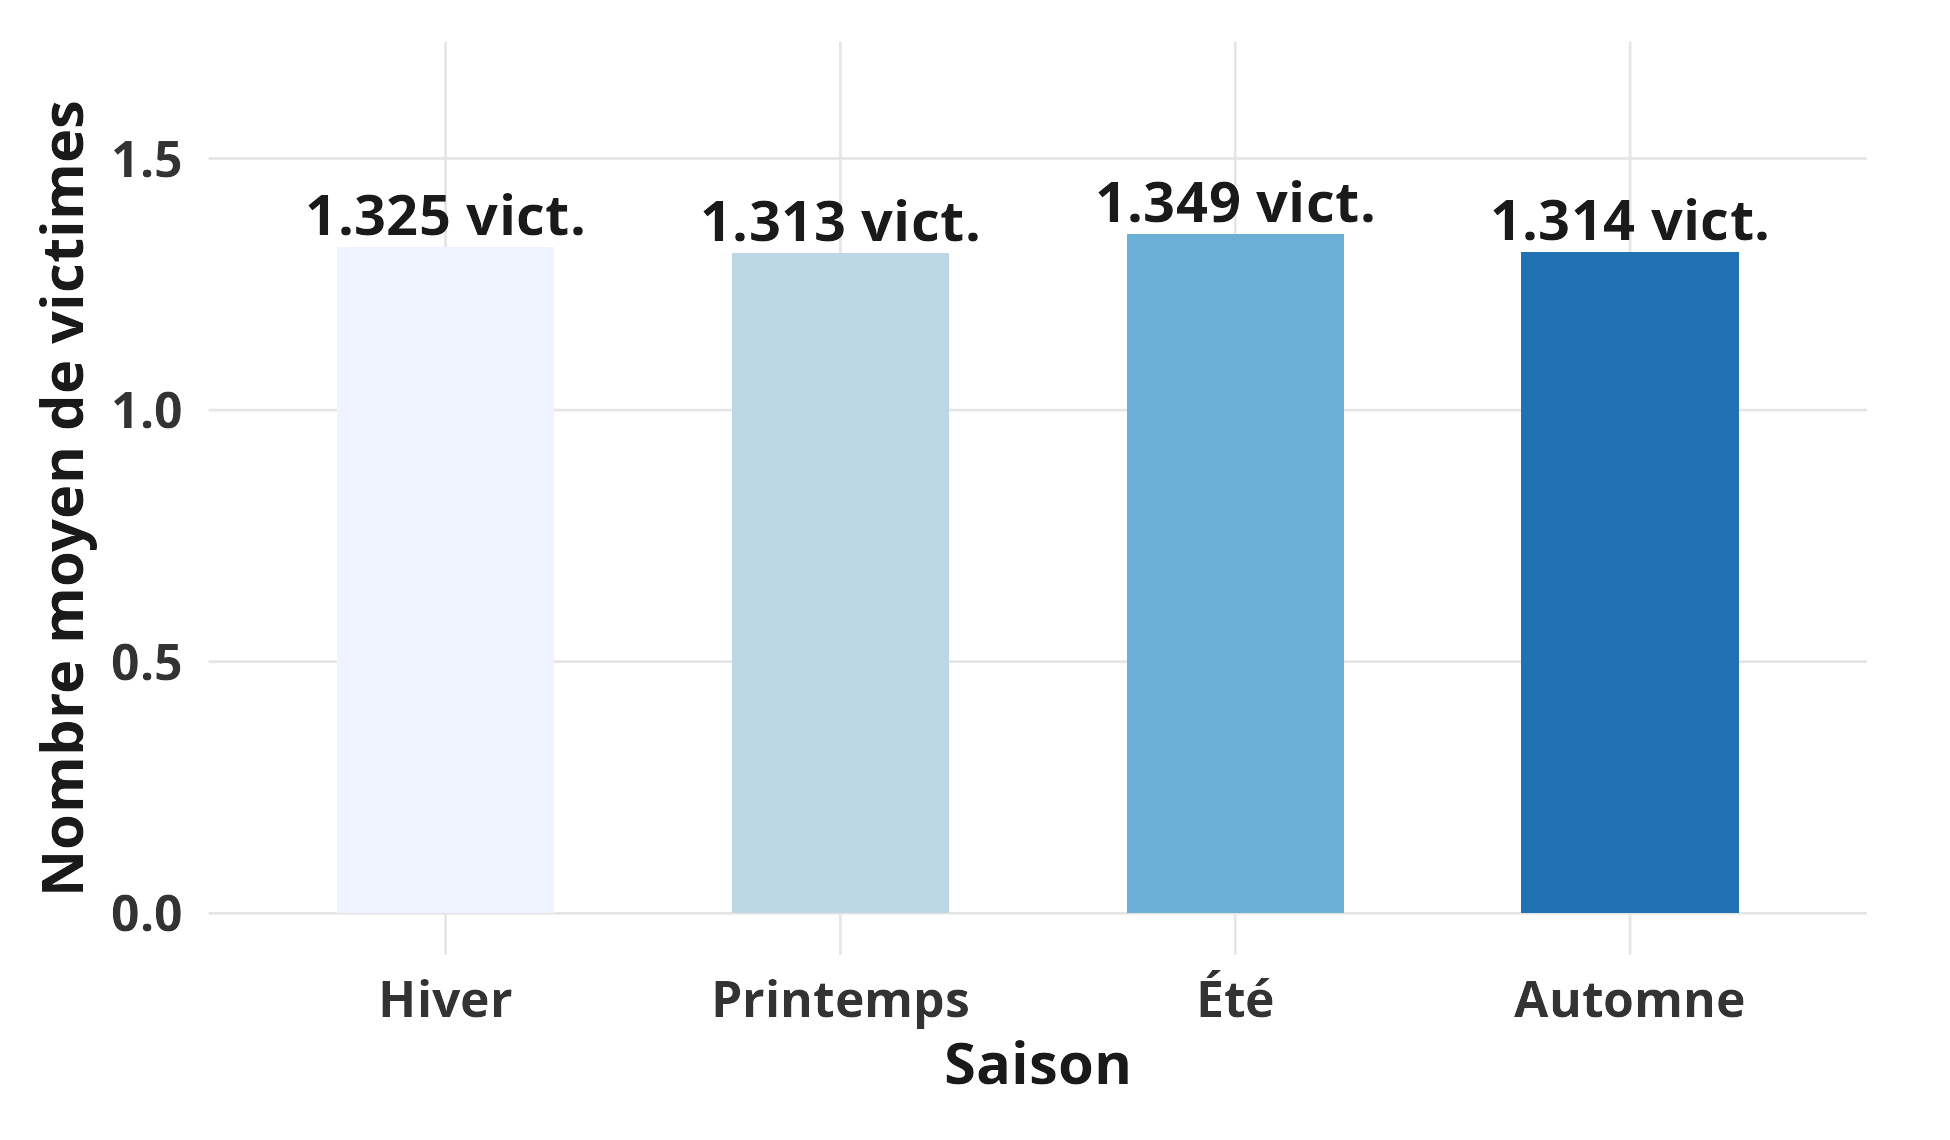
\includegraphics[width=0.65\linewidth]{biv_saison.png}
\caption{Nombre moyen de victimes par accident selon la saison (valeurs moyennes en têtes de barres).}
\label{fig:biv_saison}
\end{figure}

\noindent\textbf{Démarche d'inférence statistique :}
\begin{enumerate}
    \item \textit{Test de normalité :} Le test de Kolmogorov-Smirnov rejette formellement la normalité dans chaque saison ($p < 2{,}2 \times 10^{-16}$). Ce test est indicatif : la variable est discrète et comporte de nombreuses valeurs identiques.
    \item \textit{Test d'homoscédasticité :} Le test de Bartlett rejette l'égalité des variances ($K^2 = 121{,}53$, $\text{df} = 3$, $p = 3{,}61 \times 10^{-26}$).
    \item \textit{Test non-paramétrique de Kruskal-Wallis :} 
    \[
    H_0 : \text{Les distributions du nombre de victimes sont identiques} \quad \text{vs} \quad H_1 : \text{Au moins une saison diffère}
    \]
    La statistique vaut $\chi^2 = 17{,}44$, $\text{df} = 3$, $p = 5{,}73 \times 10^{-4}$. On rejette $H_0$. L'été a la moyenne la plus élevée ($1{,}35$ victime contre $1{,}31$ à $1{,}33$ les autres saisons) ; l'écart est faible.
    \item \textit{Test de Welch (variances inégales) :} $F = 5{,}18$ (ddl $3$ et $27\,707$), $p = 0{,}0014$ : même conclusion que Kruskal-Wallis.
\end{enumerate}

\subsubsection{Conditions atmosphériques ($Y \sim \text{\texttt{atm\_label}}$)}

Le test de Kruskal-Wallis sur les 9 modalités météorologiques indique une hétérogénéité significative ($\chi^2 = 70{,}70$, $\text{df} = 8$, $p = 3{,}57 \times 10^{-12}$). Toutefois, l'amplitude réelle des écarts est très modérée entre les situations courantes (Normale : $1{,}324$ ; Pluie légère : $1{,}318$) et ne s'élève que lors d'épisodes de visibilité critique (Brouillard : $1{,}525$ ; Neige/Grêle : $1{,}504$). Le test de Bartlett rejette l'égalité des variances ($K^2 = 1\,764{,}6$, ddl $= 8$, $p < 2{,}2 \times 10^{-16}$) ; le test de Welch, qui ne l'exige pas, conduit à la même conclusion que Kruskal-Wallis ($F = 6{,}04$, $p = 1{,}2 \times 10^{-7}$).

\begin{table}[H]
\centering
\small
\begin{tabular}{lcccc}
\toprule
\textbf{Condition atmosphérique} & \textbf{Effectif ($n_k$)} & \textbf{Moyenne} & \textbf{Médiane} & \textbf{Écart-type} \\
\midrule
Normale           & $38\,394$ & $1{,}324$ & 1 & $0{,}837$ \\
Pluie légère      & $6\,464$  & $1{,}318$ & 1 & $0{,}777$ \\
Temps nuageux     & $2\,313$  & $1{,}299$ & 1 & $1{,}009$ \\
Pluie forte       & $1\,364$  & $1{,}367$ & 1 & $0{,}802$ \\
Temps éblouissant & $785$     & $1{,}239$ & 1 & $0{,}654$ \\
Brouillard        & $526$     & $\mathbf{1{,}525}$ & 1 & $0{,}929$ \\
Autre             & $242$     & $1{,}417$ & 1 & $0{,}908$ \\
Neige / Grêle     & $232$     & $1{,}504$ & 1 & $2{,}580$ \\
Vent fort         & $166$     & $1{,}398$ & 1 & $0{,}793$ \\
\bottomrule
\end{tabular}
\caption{Nombre moyen de victimes selon les conditions météorologiques ($\chi^2 = 70{,}70$, $\text{df} = 8$, $p = 3{,}57 \times 10^{-12}$).}
\label{tab:biv_atm}
\end{table}

\begin{figure}[H]
\centering
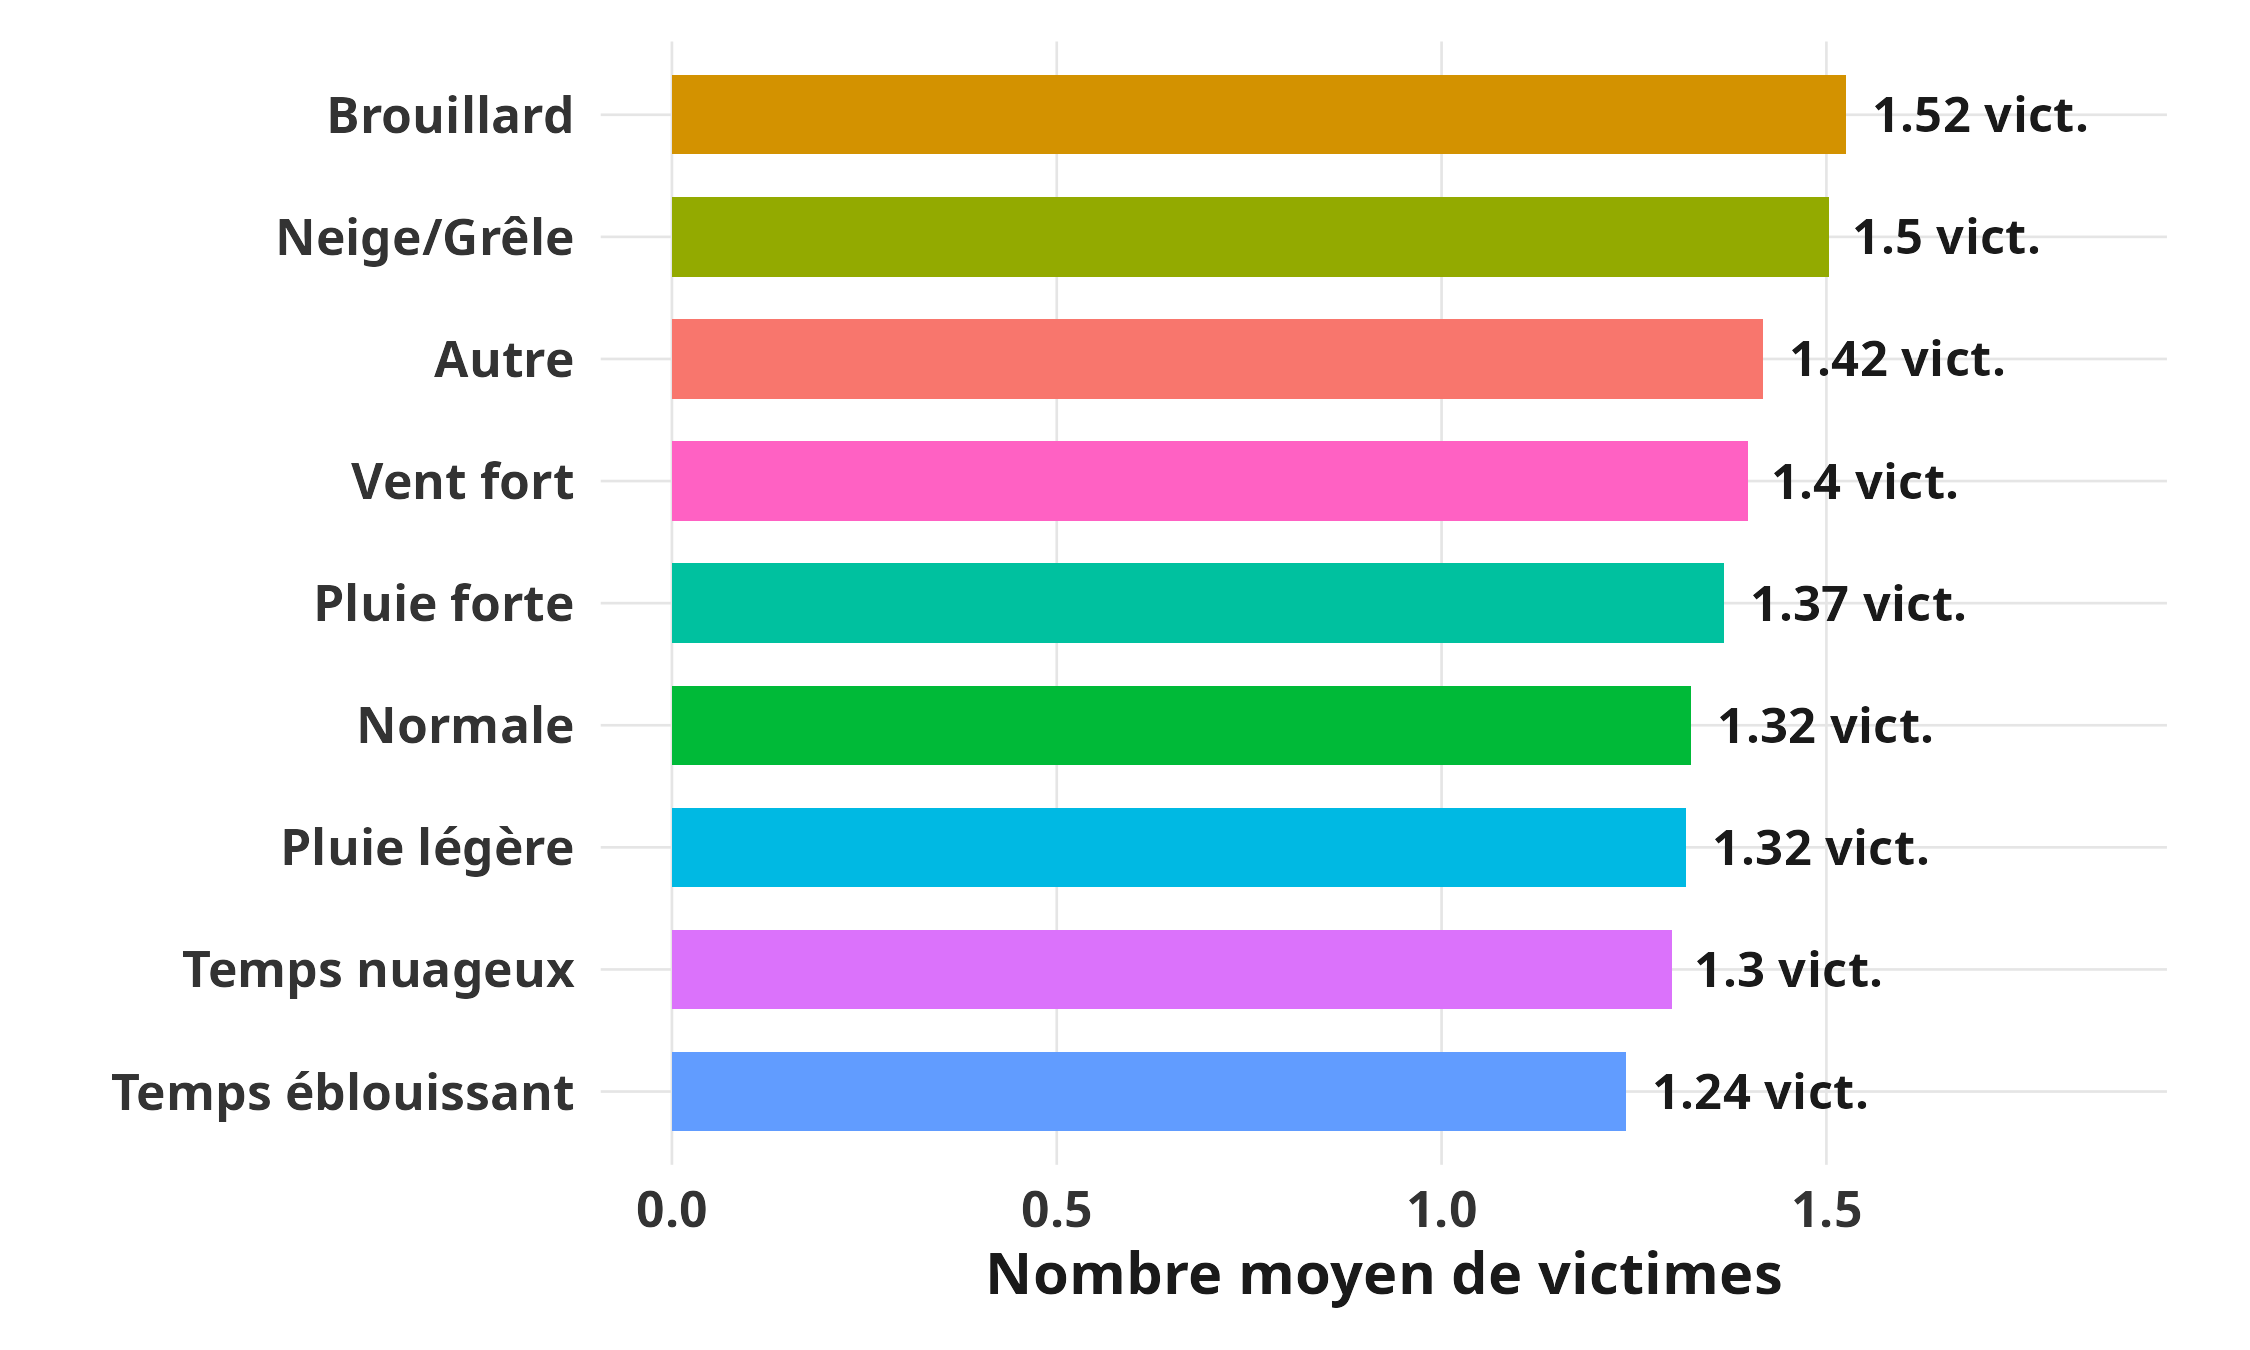
\includegraphics[width=0.75\linewidth]{biv_atm.png}
\caption{Nombre moyen de victimes selon les conditions atmosphériques.}
\label{fig:biv_atm}
\end{figure}

\subsubsection{Localisation en/hors agglomération ($Y \sim \text{\texttt{agg\_label}}$)}

La zone constitue un déterminant majeur du nombre de victimes. Le test non-paramétrique de Wilcoxon-Mann-Whitney confirme une différence hautement significative ($W = 251\,213\,904$, $p < 2{,}2 \times 10^{-16}$). La vitesse plus élevée hors agglomération majore fortement l'énergie cinétique et le nombre de victimes par collision. Le test de Fisher rejette l'égalité des variances ($F = 0{,}316$, $p < 2{,}2 \times 10^{-16}$ ; variances de $0{,}39$ en agglomération et de $1{,}24$ hors agglomération) ; le test $t$ de Welch conduit à la même conclusion que Wilcoxon-Mann-Whitney ($t = -32{,}0$, $p < 2{,}2 \times 10^{-16}$).

\begin{table}[H]
\centering
\small
\begin{tabular}{lccccc}
\toprule
\textbf{Zone géographique} & \textbf{Effectif ($n_k$)} & \textbf{Moyenne} & \textbf{Médiane} & \textbf{Écart-type} & \textbf{Test de Wilcoxon} \\
\midrule
En agglomération    & $31\,739$ & $1{,}220$ & 1 & $0{,}627$ & \multirow{2}{*}{$W = 251\,213\,904$ ($p < 2{,}2 \times 10^{-16}$)} \\
Hors agglomération  & $18\,747$ & $\mathbf{1{,}504}$ & 1 & $1{,}115$ & \\
\bottomrule
\end{tabular}
\caption{Comparaison du nombre de victimes en agglomération vs hors agglomération ($n = 50\,486$).}
\label{tab:biv_agg}
\end{table}

\begin{figure}[H]
\centering
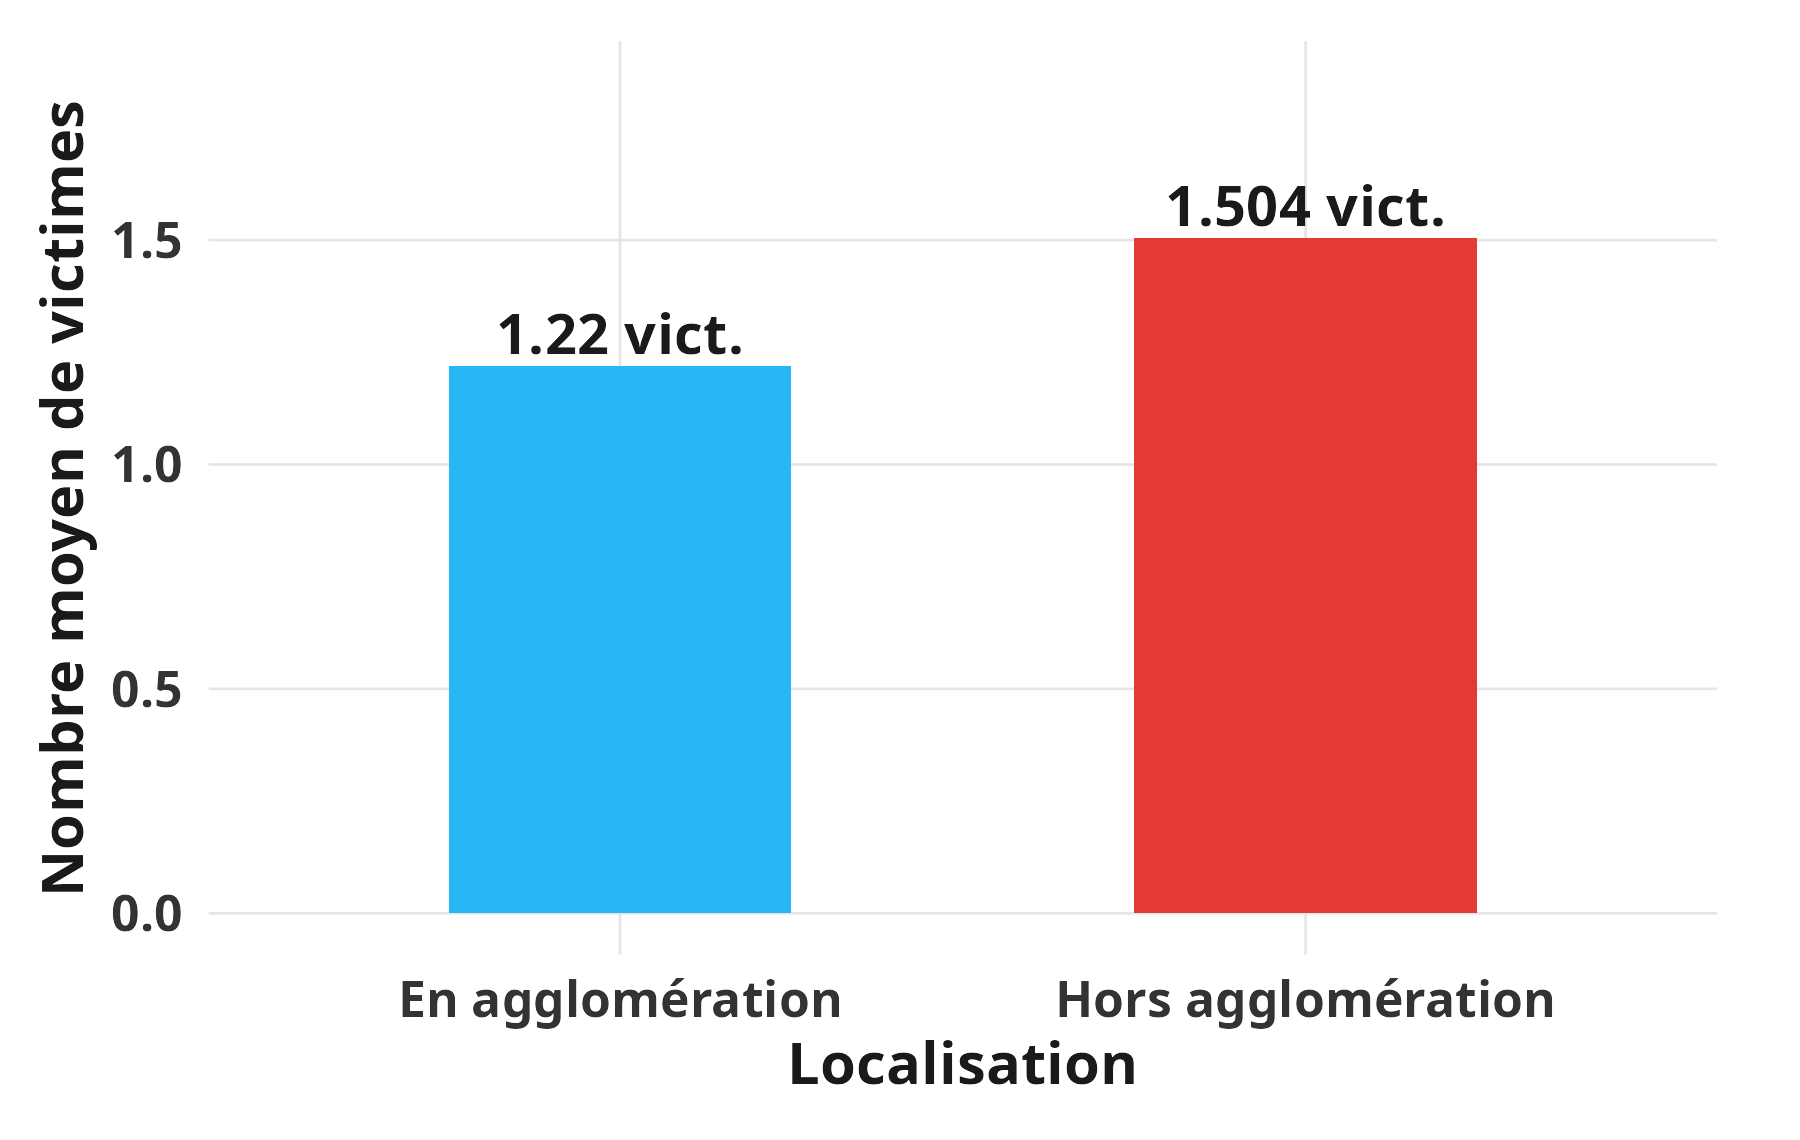
\includegraphics[width=0.55\linewidth]{biv_agg.png}
\caption{Nombre moyen de victimes selon la zone géographique.}
\label{fig:biv_agg}
\end{figure}

\subsubsection{Conditions de luminosité ($Y \sim \text{\texttt{lum\_label}}$)}

La luminosité présente un impact marqué sur la gravité des accidents. Le test de Kruskal-Wallis rejette très largement l'homogénéité des distributions ($\chi^2 = 378{,}59$, $\text{df} = 4$, $p < 2{,}2 \times 10^{-16}$). La nuit sans éclairage public génère le pic de gravité le plus prononcé ($\mu = 1{,}518$). Le test de Bartlett rejette l'égalité des variances ($K^2 = 2\,275{,}6$, ddl $= 4$, $p < 2{,}2 \times 10^{-16}$).

\begin{table}[H]
\centering
\small
\begin{tabular}{lcccc}
\toprule
\textbf{Condition d'éclairage} & \textbf{Effectif ($n_k$)} & \textbf{Moyenne} & \textbf{Médiane} & \textbf{Écart-type} \\
\midrule
Plein jour             & $33\,097$ & $1{,}297$ & 1 & $0{,}786$ \\
Nuit éclairage allumé  & $7\,829$  & $1{,}303$ & 1 & $0{,}741$ \\
Nuit sans éclairage    & $5\,617$  & $\mathbf{1{,}518}$ & 1 & $1{,}111$ \\
Crépuscule / aube      & $3\,379$  & $1{,}325$ & 1 & $1{,}122$ \\
Nuit, éclairage public non allumé & $564$ & $1{,}429$ & 1 & $0{,}978$ \\
\bottomrule
\end{tabular}
\caption{Nombre moyen de victimes selon les conditions de luminosité ($\chi^2 = 378{,}59$, $\text{df} = 4$, $p < 2{,}2 \times 10^{-16}$).}
\label{tab:biv_lum}
\end{table}

\begin{figure}[H]
\centering
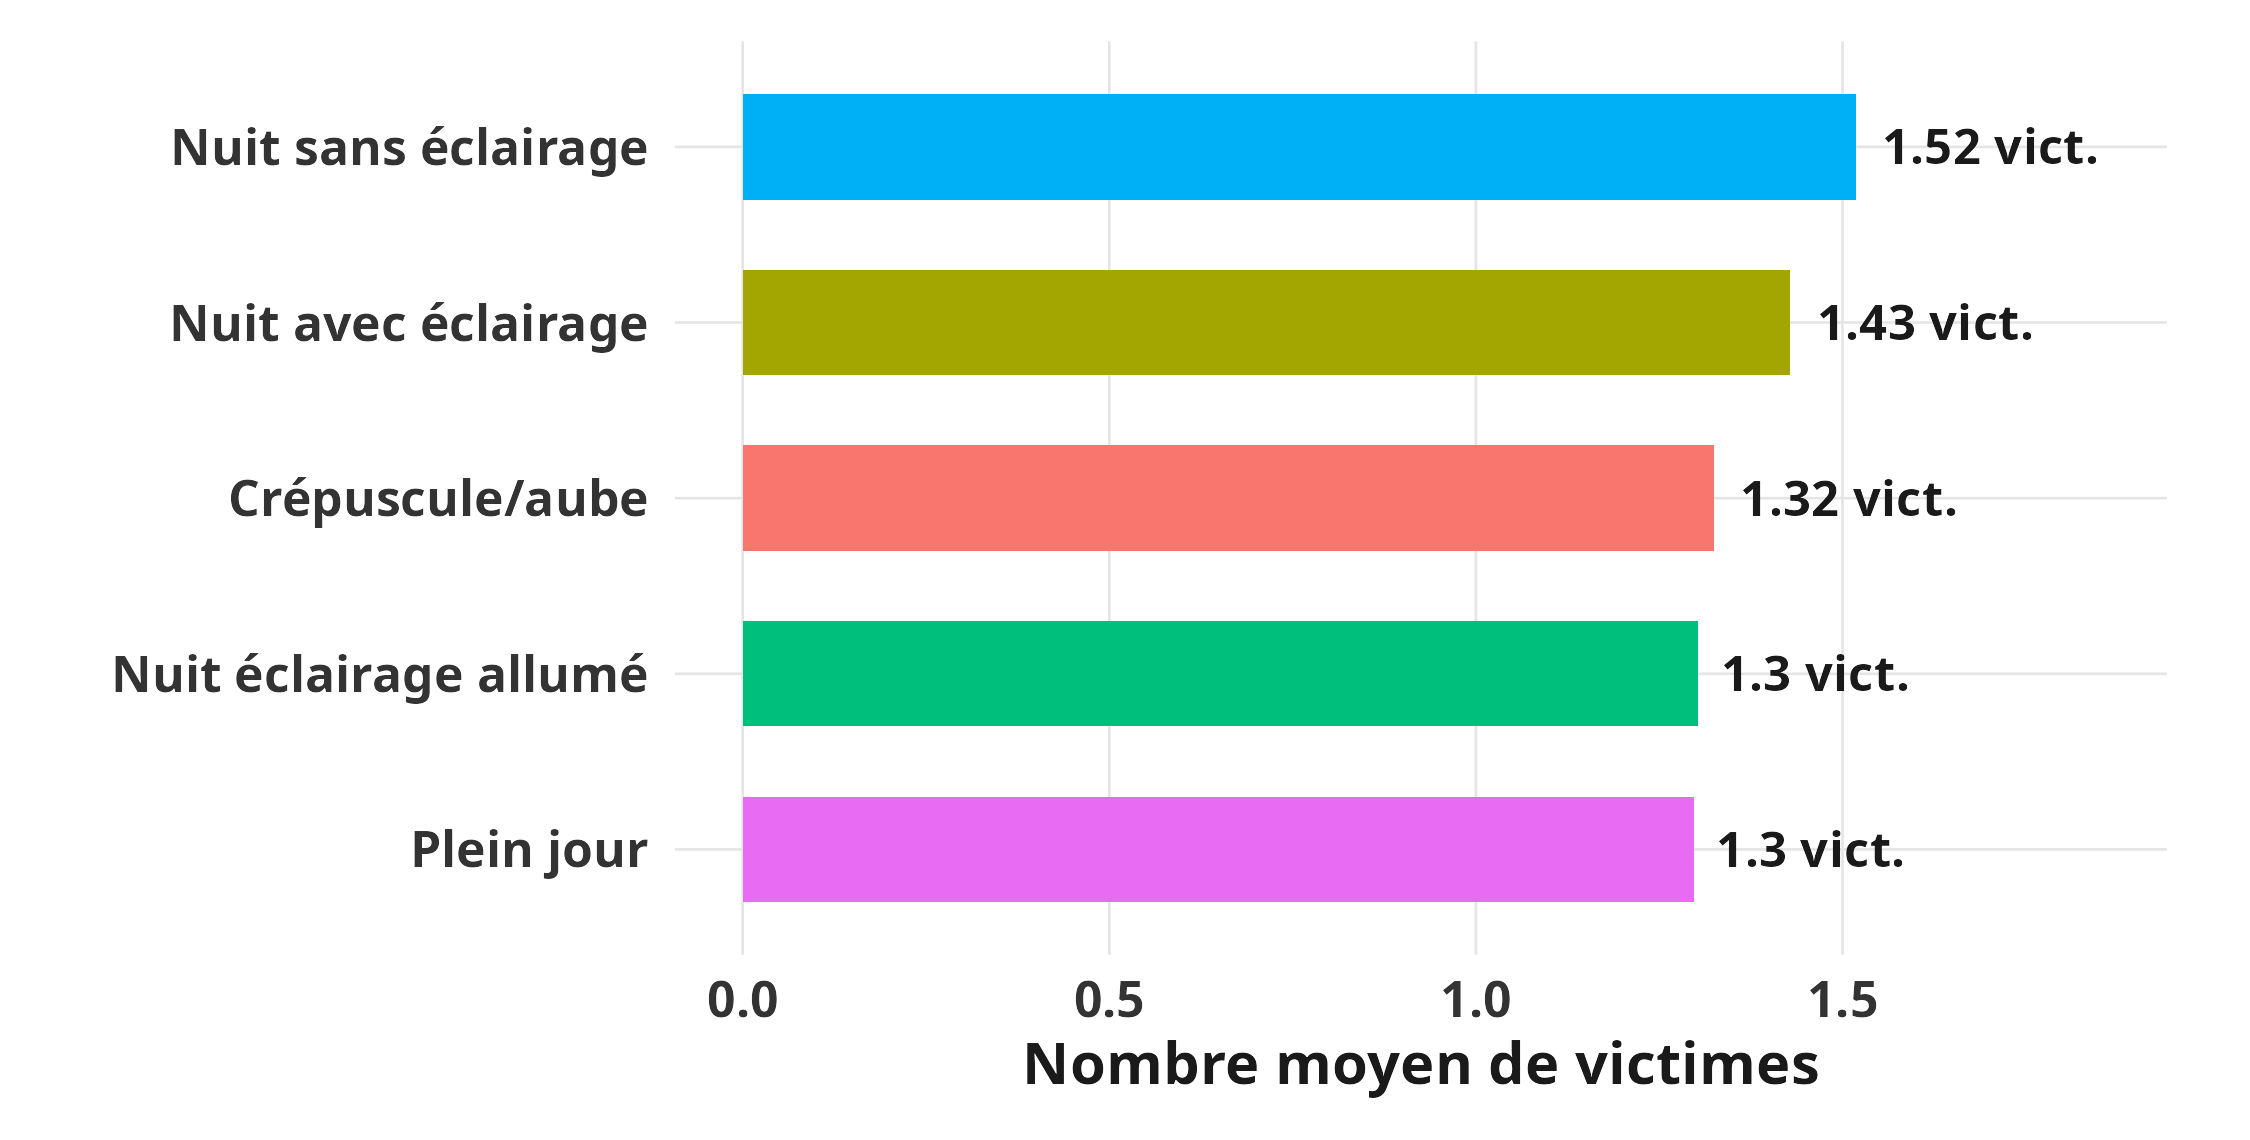
\includegraphics[width=0.75\linewidth]{biv_lum.png}
\caption{Nombre moyen de victimes selon les conditions de luminosité.}
\label{fig:biv_lum}
\end{figure}

\subsubsection{Typologie de collision ($Y \sim \text{\texttt{col\_regroup}}$)}

Le type de collision est le déterminant physique le plus discriminant de la gravité corporelle ($\chi^2 = 3\,456{,}4$, $\text{df} = 5$, $p < 2{,}2 \times 10^{-16}$). Les collisions multiples à 3 véhicules ou plus ($\mu = 2{,}075$) et les collisions en chaîne ($\mu = 1{,}735$) démultiplient les victimes, suivies des chocs frontaux à 2 véhicules ($\mu = 1{,}632$). Pour les collisions à deux véhicules, les chocs par l'arrière ($\mu = 1{,}259$) et par le côté ($\mu = 1{,}334$) sont regroupés en une modalité commune : il s'agit de deux configurations sans choc frontal direct dont l'écart de gravité ($0{,}075$ victime) est très faible devant la sur-gravité d'un choc frontal ($+0{,}35$ victime), bien que leur différence soit statistiquement significative compte tenu de la très grande puissance du test sur $50\,486$ observations (Mann-Whitney, $p \approx 10^{-15}$).

\begin{table}[H]
\centering
\small
\begin{tabular}{lcccc}
\toprule
\textbf{Typologie de collision} & \textbf{Effectif ($n_k$)} & \textbf{Moyenne} & \textbf{Médiane} & \textbf{Écart-type} \\
\midrule
Trois véh.+ coll. multiples & $1\,424$  & $\mathbf{2{,}075}$ & 2 & $1{,}899$ \\
Trois véh.+ en chaîne       & $1\,714$  & $1{,}735$ & 1 & $1{,}110$ \\
Deux véh. - Frontale        & $5\,533$  & $1{,}632$ & 1 & $1{,}013$ \\
Deux véh. - Arrière / Côté  & $21\,838$ & $1{,}282$ & 1 & $0{,}712$ \\
Autre collision             & $14\,948$ & $1{,}205$ & 1 & $0{,}725$ \\
Sans collision              & $5\,029$  & $1{,}185$ & 1 & $0{,}762$ \\
\bottomrule
\end{tabular}
\caption{Nombre moyen de victimes par type de collision ($\chi^2 = 3\,456{,}4$, $\text{df} = 5$, $p < 2{,}2 \times 10^{-16}$).}
\label{tab:biv_col}
\end{table}

\begin{figure}[H]
\centering
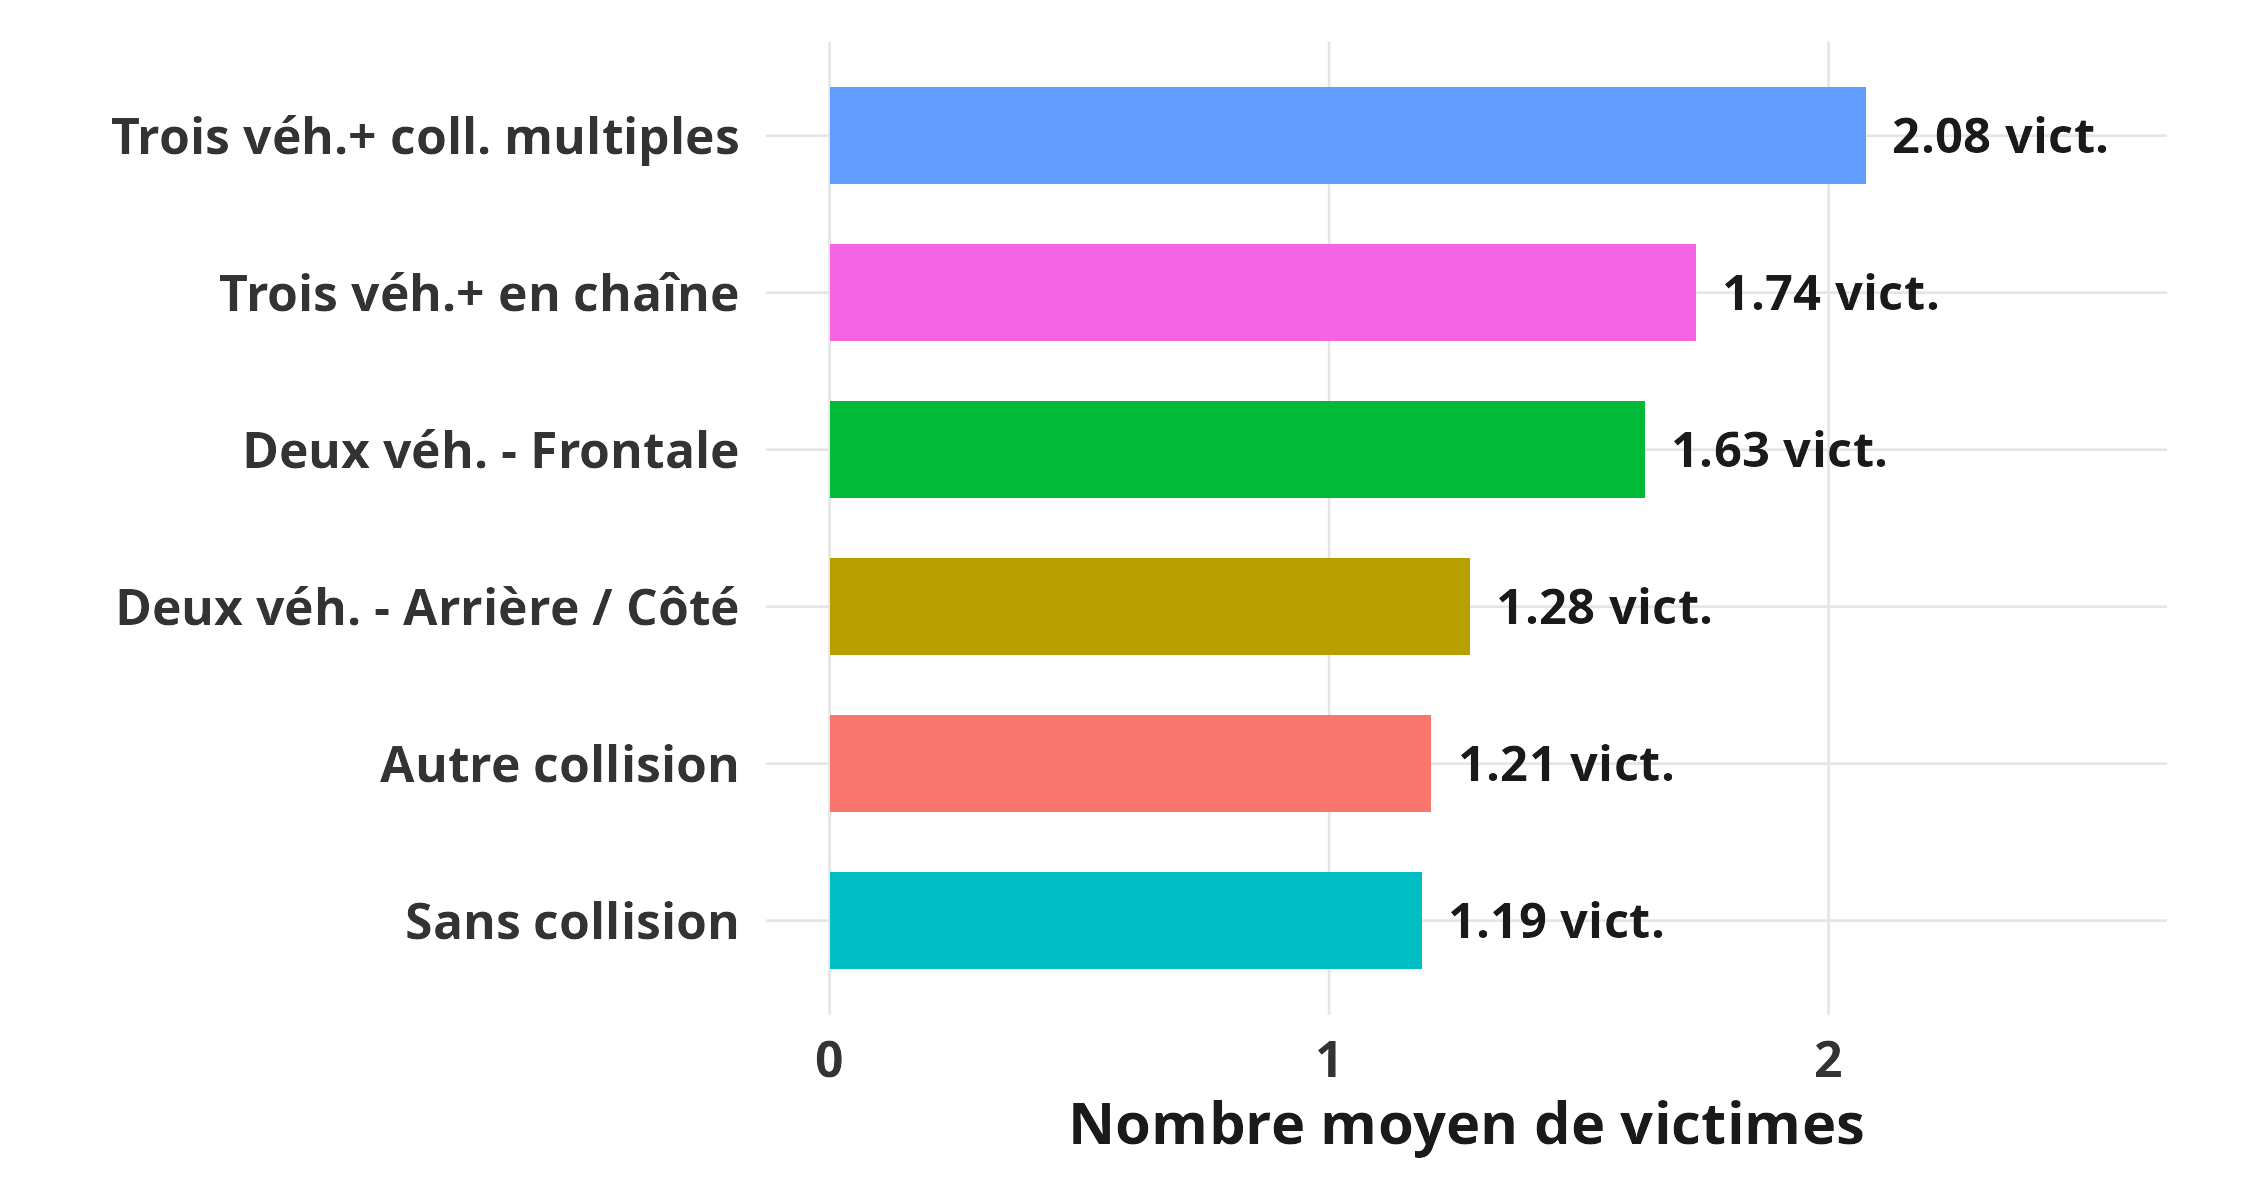
\includegraphics[width=0.75\linewidth]{biv_col.png}
\caption{Nombre moyen de victimes par typologie de collision.}
\label{fig:biv_col}
\end{figure}

\subsubsection{Facteurs humains, cinétiques et d'équipement}

L'enrichissement de la base avec les caractéristiques usagers et les obstacles permet d'isoler des facteurs de vulnérabilité majeurs. Comme la distribution de $Y$ est asymétrique dans chaque sous-groupe, nous appliquons le test bilatéral de Wilcoxon-Mann-Whitney pour chaque facteur dichotomique :
\begin{table}[H]
\centering
\footnotesize
\resizebox{\linewidth}{!}{%
\begin{tabular}{lcccc}
\toprule
\textbf{Facteur explicatif ($X$)} & \textbf{Moyenne avec ($X=1$)} & \textbf{Moyenne sans ($X=0$)} & \textbf{Statistique $W$} & \textbf{$p$-valeur} \\
\midrule
Jeune 18--24 ans impliqué   & $\mathbf{1{,}496}$ & $1{,}246$ & $240\,797\,498$ & $< 2{,}2 \times 10^{-16}$ *** \\
Choc contre obstacle fixe   & $\mathbf{1{,}408}$ & $1{,}300$ & $219\,798\,484$ & $4{,}34 \times 10^{-31}$ *** \\
Au moins un conducteur masculin & $\mathbf{1{,}342}$ & $1{,}229$ & $148\,040\,555$ & $< 2{,}2 \times 10^{-16}$ *** \\Senior 65 ans+ impliqué     & $\mathbf{1{,}363}$ & $1{,}315$ & $210\,820\,447$ & $1{,}39 \times 10^{-6}$ *** \\
Chaussée mouillée / glissante & $\mathbf{1{,}349}$ & $1{,}319$ & $218\,740\,904$ & $0{,}0237$ * \\
Non-port documenté ceinture / casque & $\mathbf{1{,}694}$ & $1{,}316$ & $26\,400\,163$ & $< 2{,}2 \times 10^{-16}$ *** \\
\bottomrule
\end{tabular}}
\caption{Tests non-paramétriques de Wilcoxon-Mann-Whitney sur les facteurs comportementaux et structurels ($n = 50\,486$).}
\label{tab:biv_humains}
\end{table} 

\noindent\textbf{Interprétation :}
\begin{itemize}
    \item La présence d'un jeune de 18 à 24 ans majore le nombre moyen de victimes de $+0{,}25$ par accident ; ces accidents impliquent aussi plus de personnes (voir section~4).
    \item La présence d'au moins un conducteur masculin est associée à un nombre moyen de victimes un peu plus élevé ($1{,}34$ contre $1{,}23$), mais cette variable dépend du nombre de véhicules : un accident à un seul véhicule compte au moins un conducteur masculin dans $73{,}5\,\%$ des cas, contre $92{,}6\,\%$ à deux véhicules et $97{,}0\,\%$ à trois véhicules ou plus. À nombre de véhicules égal, l'écart est faible (de $-0{,}03$ à $+0{,}05$ victime selon le nombre de véhicules) : l'association brute reflète donc surtout le nombre de véhicules.
    \item Le choc contre obstacle fixe (arbre, mur, glissière) augmente le nombre moyen de victimes à $1{,}41$ ($p = 4{,}34 \times 10^{-31}$).
       \item Les accidents avec un non-port documenté de ceinture ou de casque comptent en moyenne $1{,}69$ victime, contre $1{,}32$ pour les autres. Ils concernent $1\,302$ accidents ; $37\,\%$ d'entre eux ont au moins deux victimes, contre $21\,\%$ des autres. L'équipement n'est évaluable que pour une partie des accidents ($6\,998$ ne le sont pas) : la valeur 0 signifie \og aucun non-port documenté\fg{}, pas \og tous équipés\fg{}.
\end{itemize}



\subsection{Liaisons entre variables qualitatives explicatives : Du $\chi^2$ au V de Cramer}

Sur un échantillon de $n = 50\,486$ accidents, le test du $\chi^2$ d'indépendance rejette systématiquement l'hypothèse nulle ($p < 2{,}2 \times 10^{-16}$), même pour des liaisons minimes. Le V de Cramer, qui mesure l'intensité de la liaison indépendamment de la taille de l'échantillon, complète le test du $\chi^2$ :
\[
V = \sqrt{\frac{\chi^2}{n \cdot \min(l-1, c-1)}}
\]

\begin{table}[H]
\centering
\footnotesize
\resizebox{\linewidth}{!}{%
\begin{tabular}{lcccl}
\toprule
\textbf{Croisement ($X_1 \times X_2$)} & \textbf{Statistique $\chi^2$} & \textbf{ddl} & \textbf{V de Cramer} & \textbf{Intensité} \\
\midrule
Luminosité $\times$ Agglomération        & $7\,786{,}9$ & 4  & $0{,}3927$ & Forte \\
Piétons impliqués $\times$ Agglomération & $3\,952{,}5$ & 1  & $0{,}2798$ & Modérée \\
Saison $\times$ Conditions météo         & $2\,796{,}9$ & 24 & $0{,}1359$ & Faible à modérée \\
Poids lourd $\times$ Type de collision   & $566{,}1$    & 5  & $0{,}1059$ & Faible à modérée \\
Conditions météo $\times$ Agglomération  & $359{,}6$    & 8  & $0{,}0844$ & Négligeable \\
Non-port documenté $\times$ Agglomération & $341{,}6$   & 1  & $0{,}0823$ & Négligeable \\
\bottomrule
\end{tabular}}
\caption{Synthèse des tests du $\chi^2$ et mesures d'intensité par le V de Cramer ($n = 50\,486$). Une liaison est jugée négligeable si $V < 0{,}10$.}
\label{tab:cramer}
\end{table}

Les liaisons les plus fortes sont celles de la luminosité avec l'agglomération ($V = 0{,}393$) et de la présence d'un piéton avec l'agglomération ($V = 0{,}280$) : des piétons sont impliqués dans $24{,}1\,\%$ des accidents en agglomération, contre $3{,}2\,\%$ hors agglomération.

\begin{figure}[H]
\centering
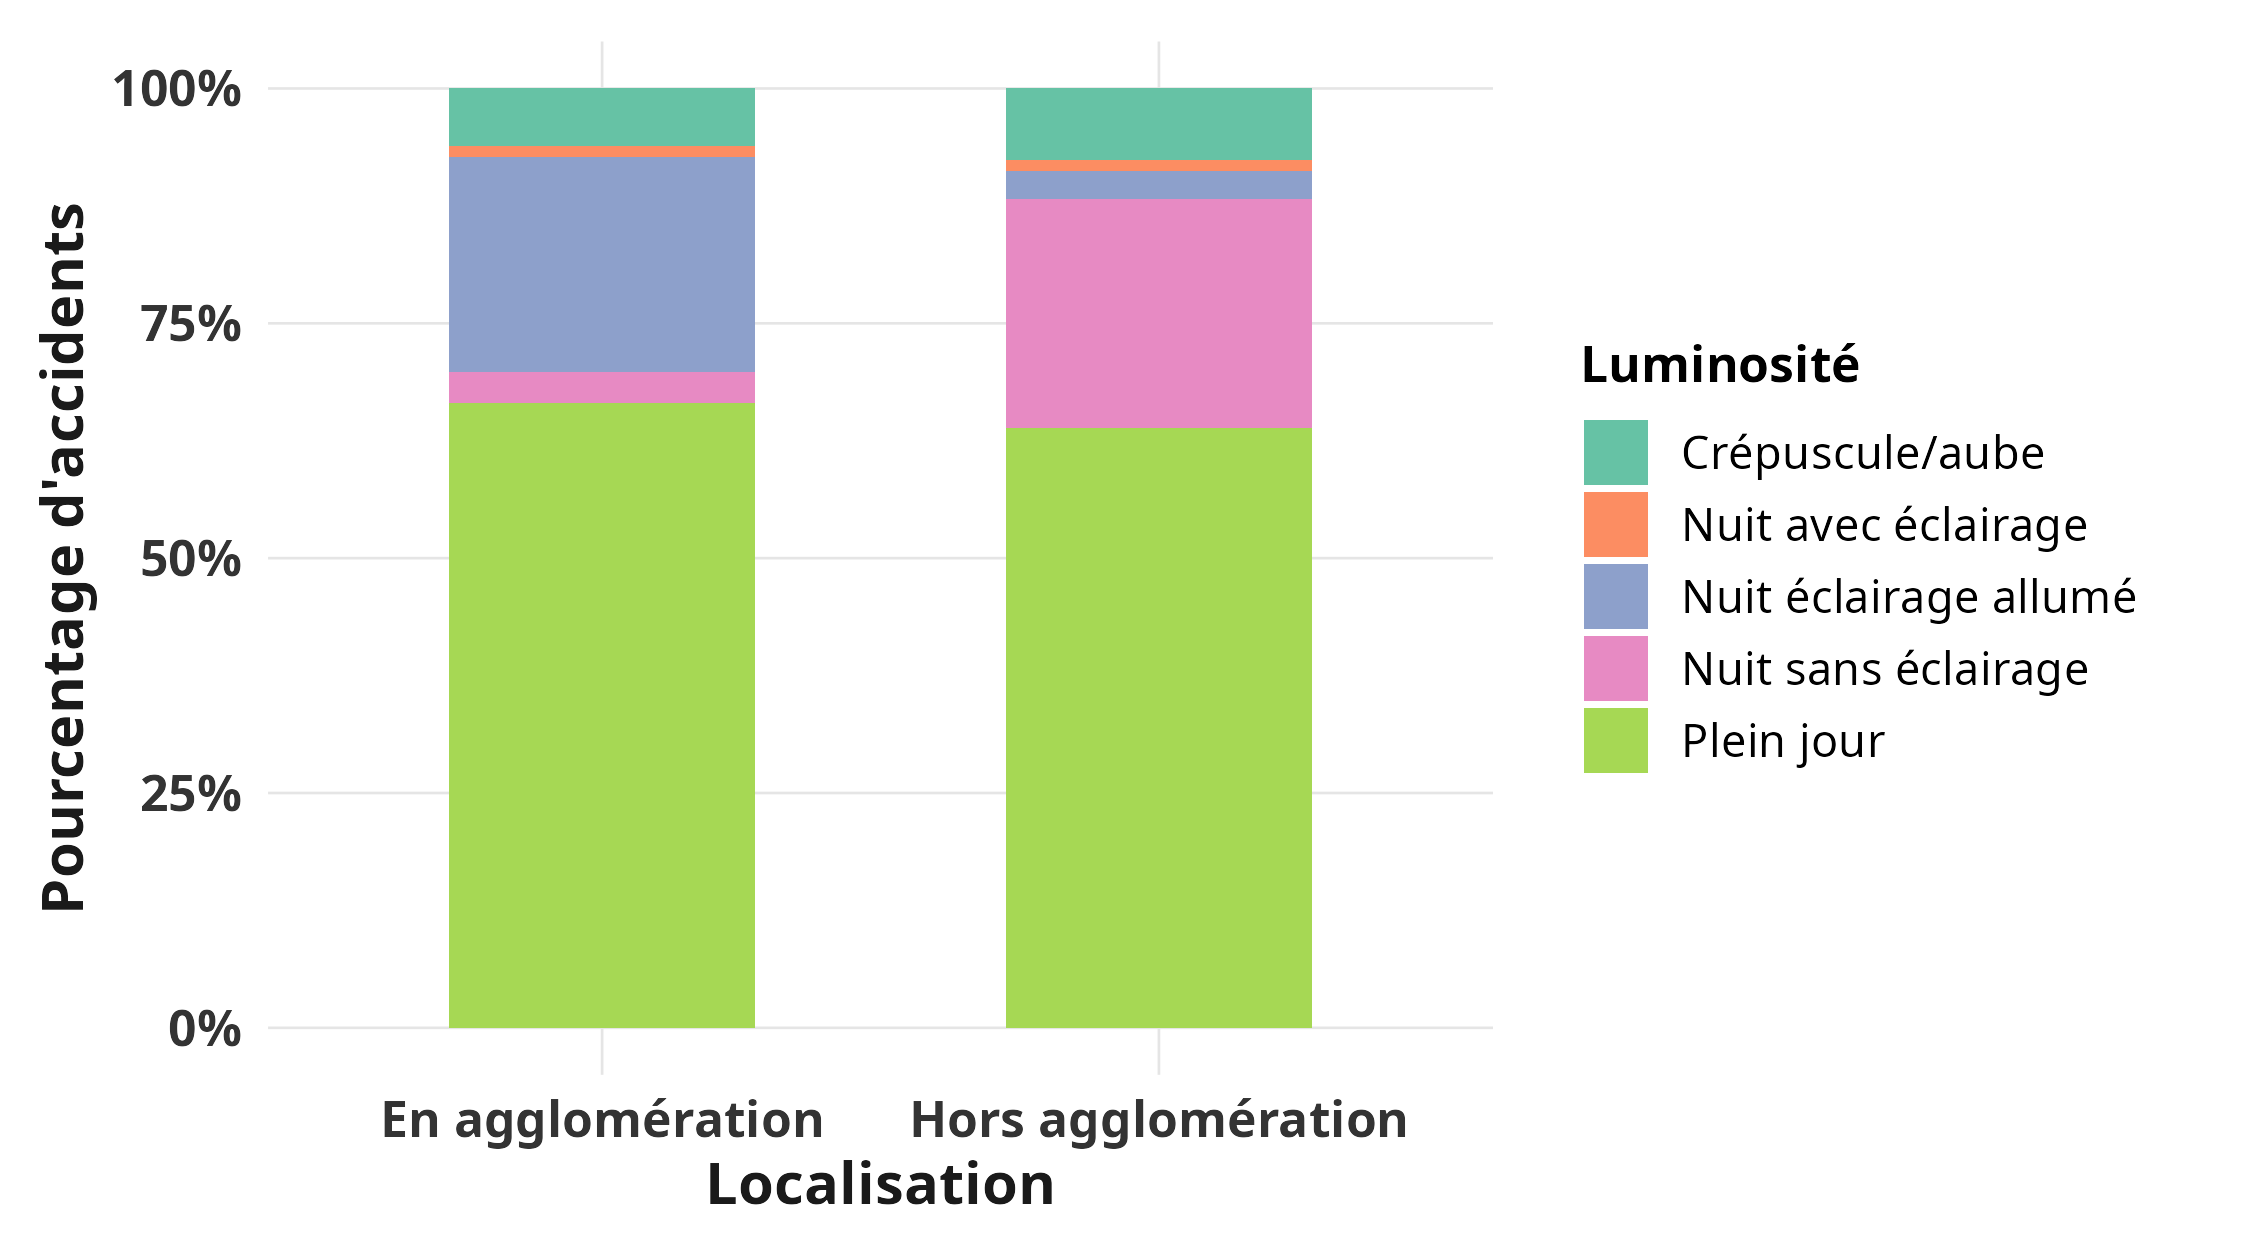
\includegraphics[width=0.75\linewidth]{cramer_lum_agg.png}
\caption{Répartition de la luminosité selon la localisation (V de Cramer = $0{,}393$).}
\label{fig:cramer_lum_agg}
\end{figure}

\noindent\textbf{Portée du V de Cramer :}
Alors que le test du $\chi^2$ qualifie le lien Météo $\times$ Zone d'\og ultra-significatif\fg{} en raison de la taille de l'échantillon, le V de Cramer ($V = 0{,}084$) indique que la météo touche de façon quasi uniforme les zones rurales et urbaines. Le non-port documenté de ceinture ou de casque est un peu plus fréquent hors agglomération ($4{,}3\,\%$ des accidents contre $1{,}6\,\%$ en agglomération), mais la liaison est très faible ($V = 0{,}082$).


\subsection{Croisement Quantitative $\times$ Quantitative : Corrélations}

Nous mesurons l'association linéaire et monotone entre les variables continues et le nombre de victimes par les coefficients de {Pearson} ($R$) et de rang de {Spearman} ($R_s$) :

\begin{table}[H]
\centering
\small
\begin{tabular}{lcccc}
\toprule
\textbf{Couple de variables quantitatives} & \textbf{Pearson ($R$)} & \textbf{$p$-value ($R$)} & \textbf{Spearman ($R_s$)} & \textbf{$p$-value ($R_s$)} \\
\midrule
VMA continue $\times$ \texttt{Nb\_victimes} & $+0{,}166$ & $< 2{,}2 \times 10^{-16}$ & ${+0{,}191}$ & $< 2{,}2 \times 10^{-16}$ \\
Âge moyen usagers $\times$ \texttt{Nb\_victimes} & $-0{,}107$ & $< 2{,}2 \times 10^{-16}$ & ${-0{,}111}$ & $< 2{,}2 \times 10^{-16}$ \\
Nb véhicules impliqués $\times$ \texttt{Nb\_victimes} & $+0{,}199$ & $< 2{,}2 \times 10^{-16}$ & ${+0{,}193}$ & $< 2{,}2 \times 10^{-16}$ \\
\bottomrule
\end{tabular}
\caption{Coefficients de corrélation linéaire et monotone avec le nombre de victimes ($n = 50\,486$).}
\label{tab:cor_quanti}
\end{table}

\begin{figure}[H]
\centering
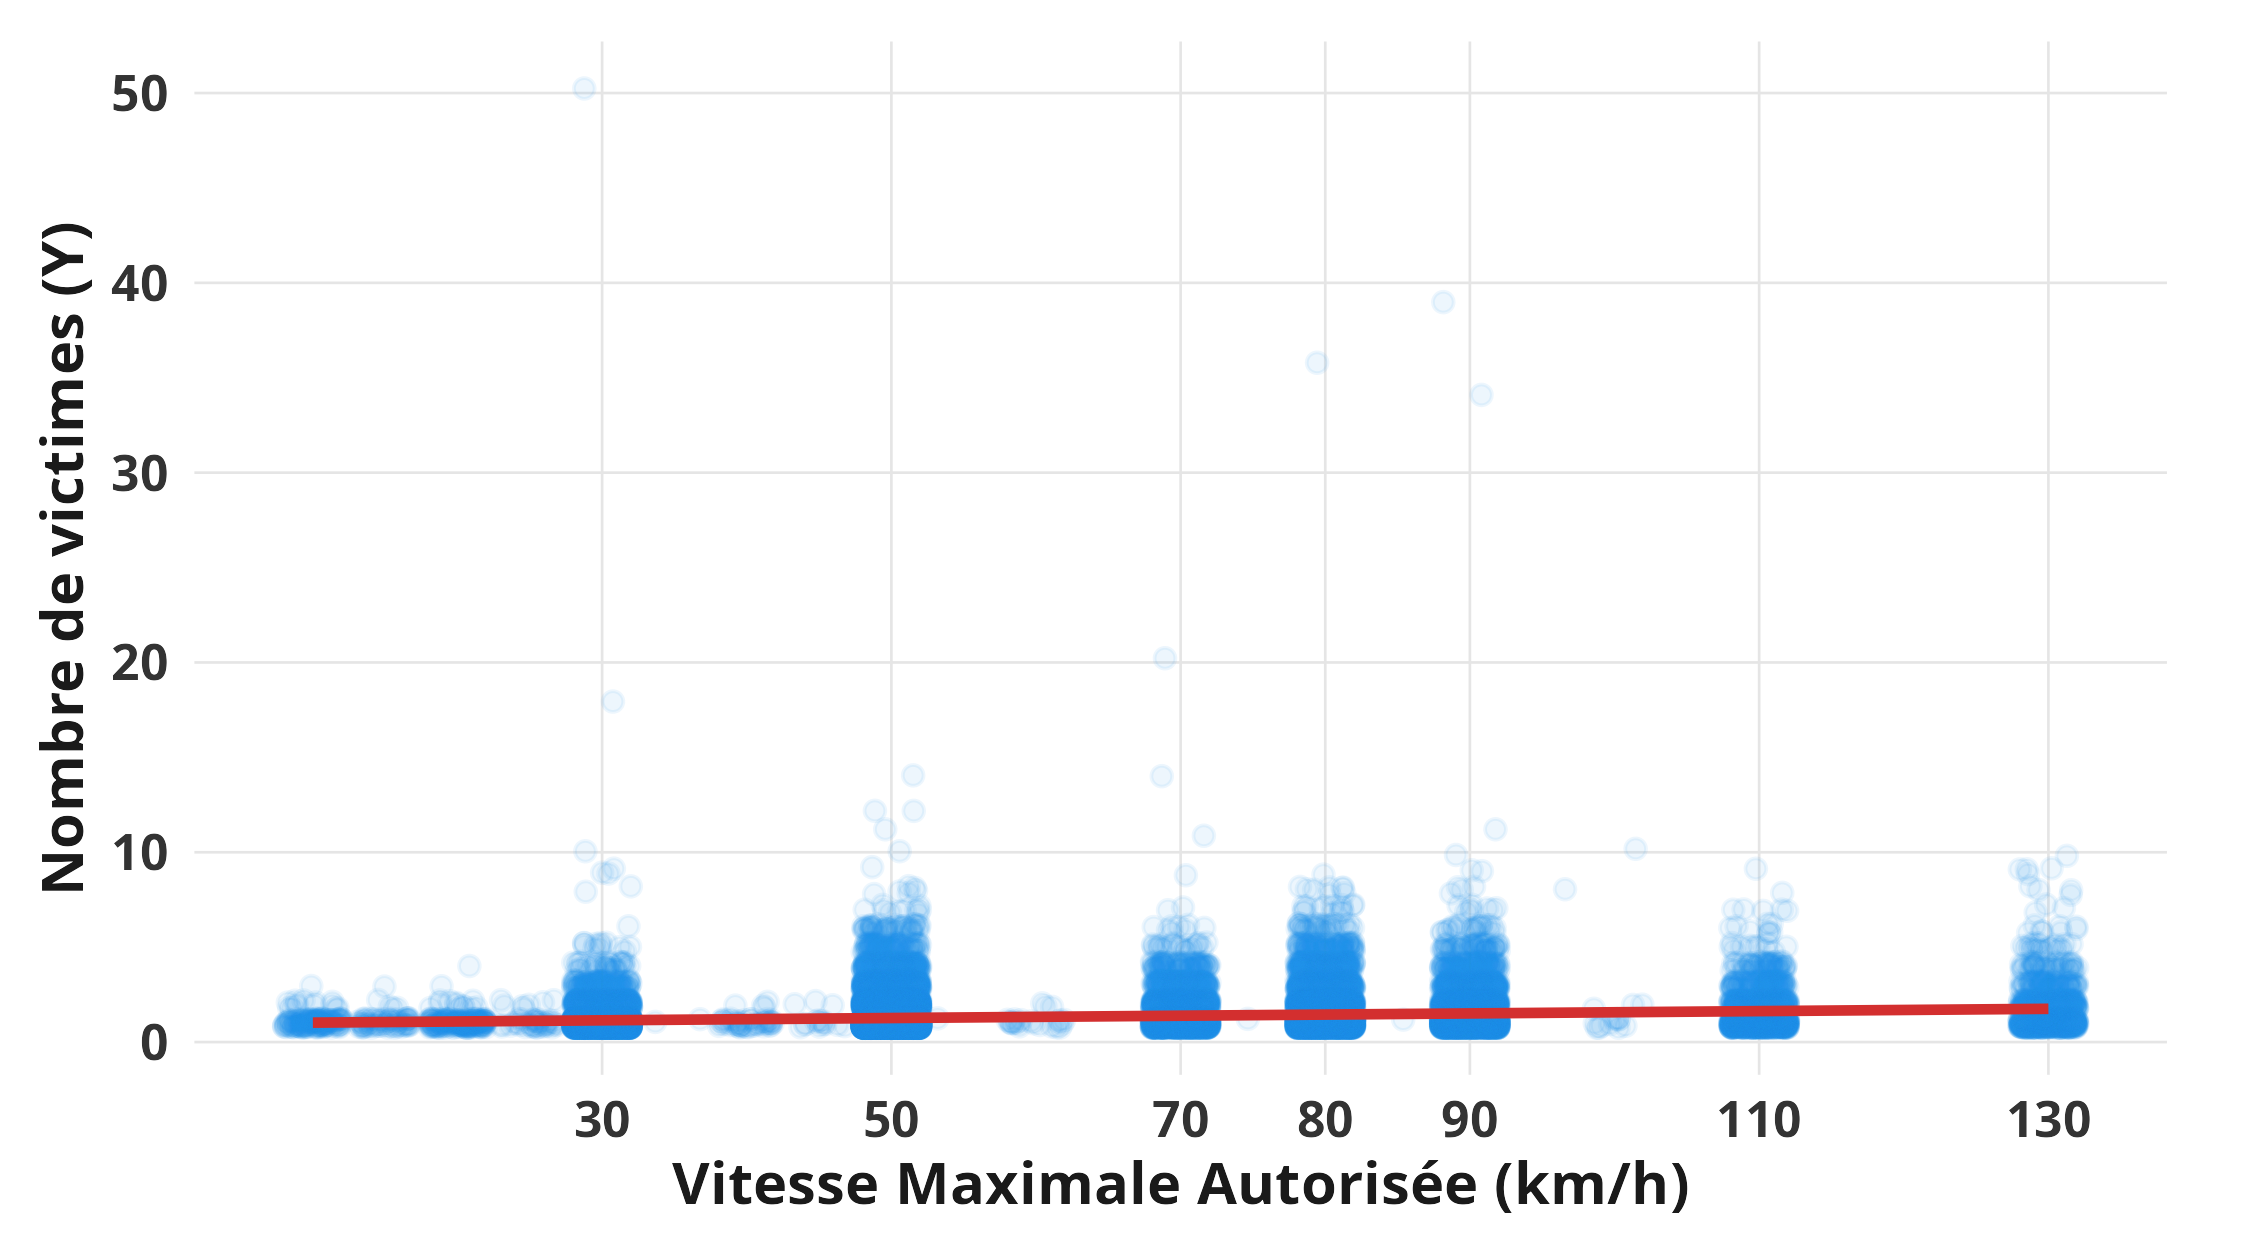
\includegraphics[width=0.7\linewidth]{quanti_vma.png}
\caption{Relation entre la vitesse autorisée (VMA continue) et le nombre de victimes.}
\label{fig:quanti_vma}
\end{figure}

\begin{figure}[H]
\centering
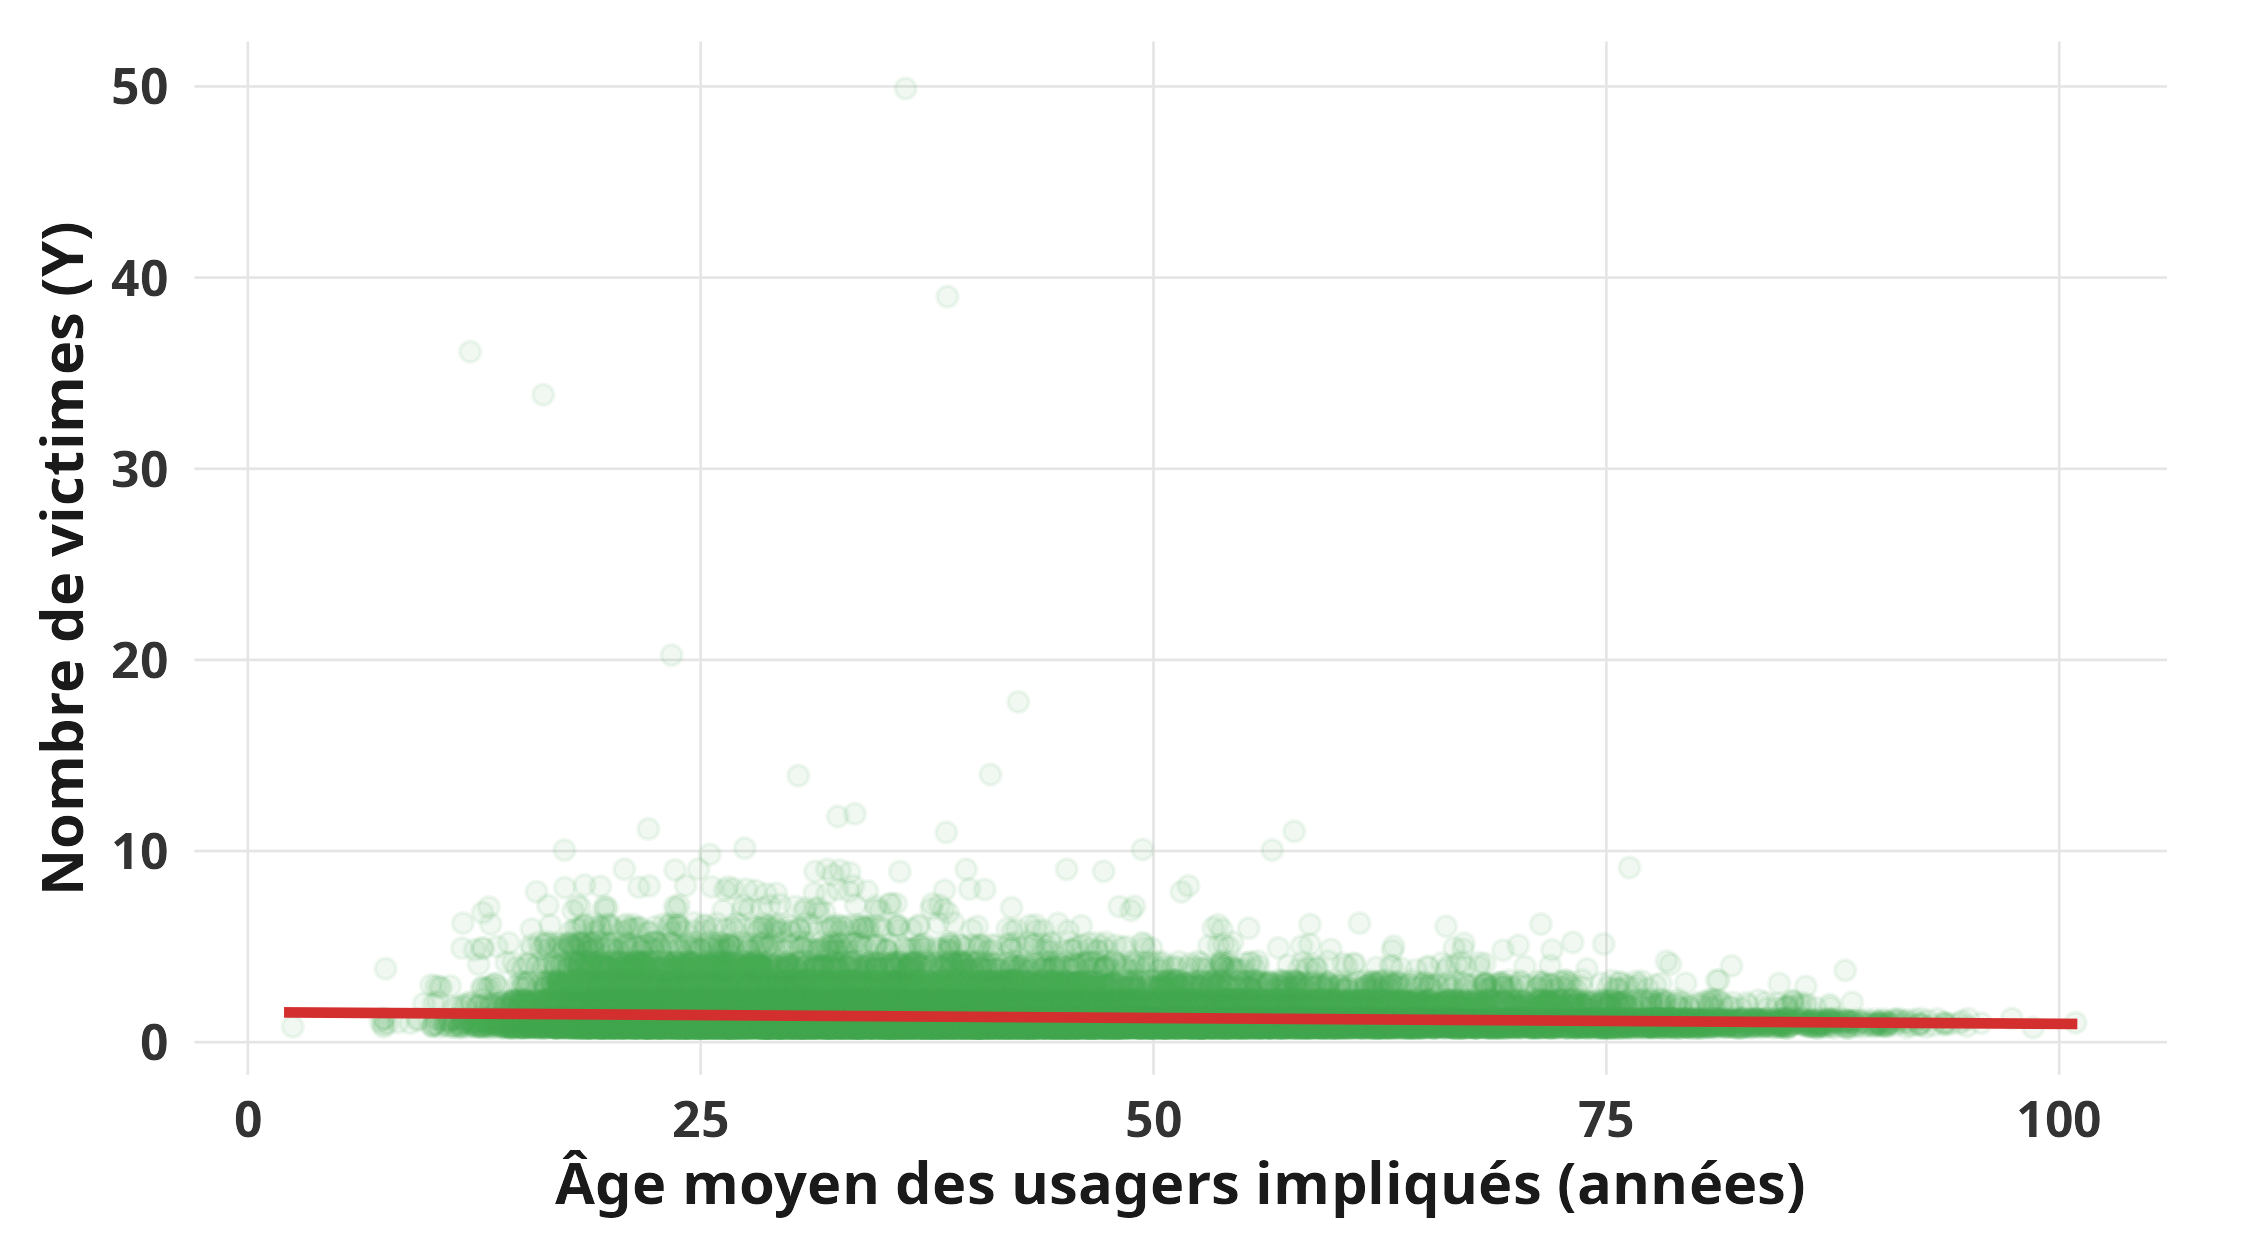
\includegraphics[width=0.7\linewidth]{quanti_age.png}
\caption{Relation entre l'âge moyen des usagers et le nombre de victimes.}
\label{fig:quanti_age}
\end{figure}

\begin{figure}[H]
\centering
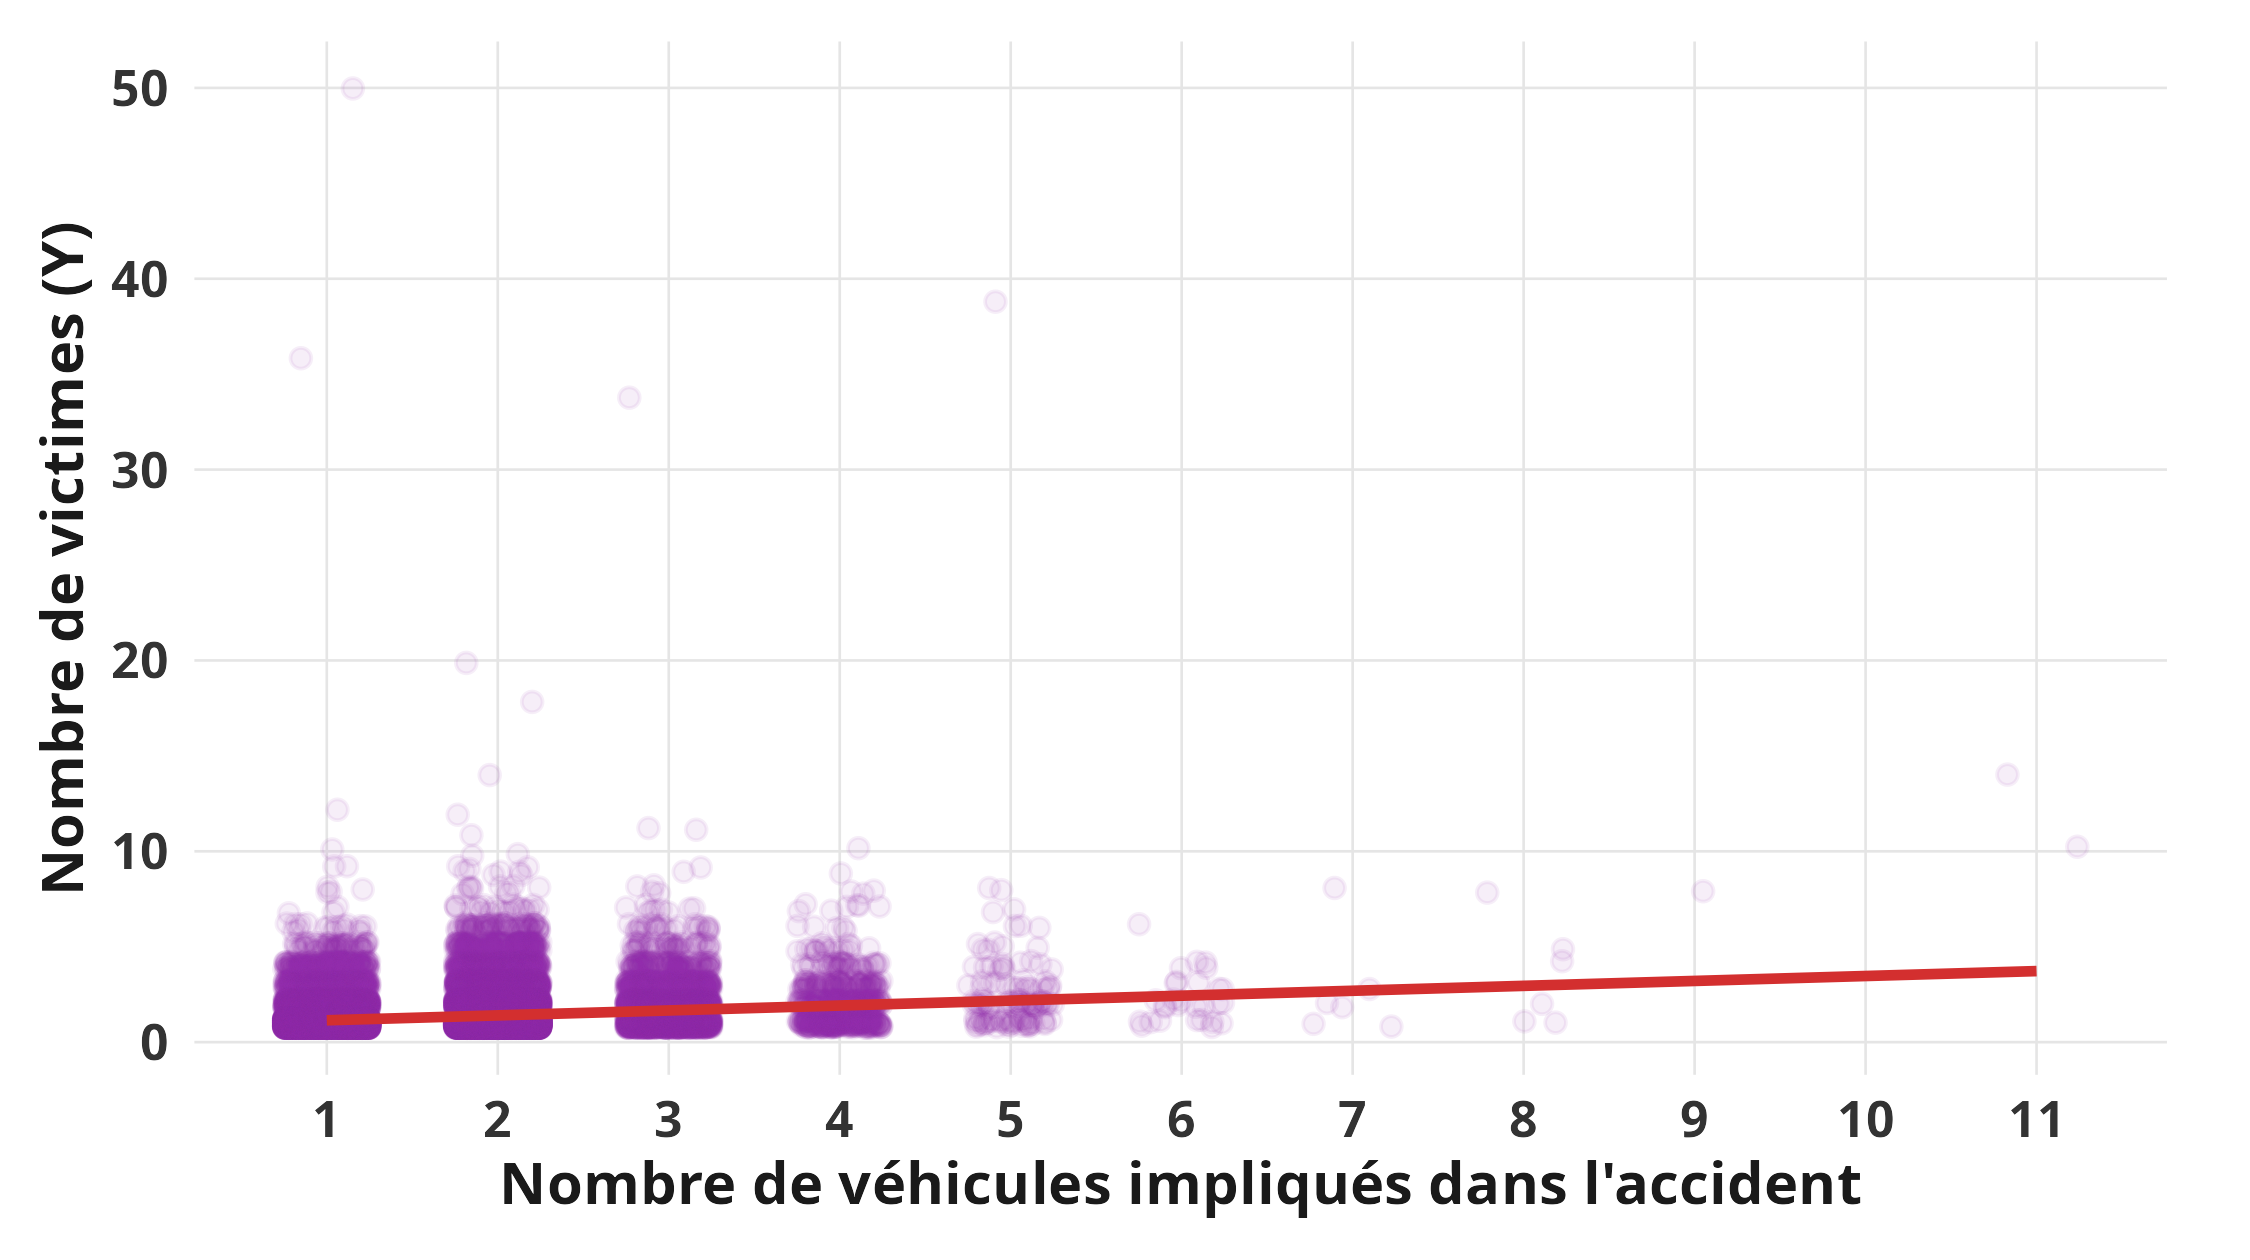
\includegraphics[width=0.7\linewidth]{quanti_vehicules.png}
\caption{Relation entre le nombre de véhicules impliqués et le nombre de victimes.}
\label{fig:quanti_vehicules}
\end{figure}

\noindent\textbf{Enseignements tirés des corrélations et des graphiques :}
\begin{itemize}
    \item \textbf{Vitesse autorisée (\texttt{vma}, $R_s = +0{,}191$) :} La corrélation positive confirme le rôle moteur de l'énergie cinétique. Sur voies rapides ($80$ à $130$\,km/h), la violence accrue des décélérations majore significativement le nombre de victimes par rapport aux zones urbaines limitées à $30$ ou $50$\,km/h.
    \item \textbf{Nombre de véhicules impliqués ($R_s = +0{,}193$) :} L'association positive traduit l'effet mécanique d'exposition : chaque véhicule additionnel apporte des occupants supplémentaires et multiplie les points d'impact (carambolages en chaîne et collisions multiples).
    \item \textbf{Âge moyen des usagers ($R_s = -0{,}111$) :} La légère corrélation négative s'explique par les modes de déplacement et le taux d'occupation des véhicules : les jeunes usagers voyagent beaucoup plus fréquemment à plusieurs (sorties collectives, trajets d'étudiants), augmentant mécaniquement le nombre de personnes exposées en cas d'accident, tandis que les usagers plus âgés effectuent majoritairement des trajets individuels ou en couple. Cette corrélation faible illustre surtout que l'impact de l'âge n'est pas linéaire, ce qui justifie d'isoler des indicatrices ciblées pour les profils extrêmes (jeunes de 18--24 ans et seniors de 65 ans et plus) plutôt que de conserver une moyenne continue.
\end{itemize}


% ==============================================================================
% SECTION 4 : MODÉLISATION LINÉAIRE MULTIPLE ET SÉLECTION DE VARIABLES
% ==============================================================================
\section{Modélisation linéaire multiple et sélection de variables}

\subsection{Échantillons d'apprentissage et de test}
Le jeu de données est partitionné une seule fois, de façon aléatoire et reproductible (\texttt{set.seed(2026)}), en un échantillon d'apprentissage ($70\,\%$, $n_{\text{app}} = 35\,340$) et un échantillon de test ($30\,\%$, $n_{\text{test}} = 15\,146$). L'étiquette de chaque accident est enregistrée dans le fichier de données : la partie~3 (Python) utilise exactement les mêmes accidents, ce qui permet de comparer les modèles sur le même jeu de test. La sélection de variables, l'estimation et les diagnostics reposent sur l'échantillon d'apprentissage ; le jeu de test ne sert qu'à évaluer les prédictions.

\subsection{Spécification du modèle}
La construction du modèle linéaire repose sur deux choix méthodologiques destinés à isoler la gravité réelle des accidents.

D'une part, nous intégrons le nombre total de personnes impliquées (\texttt{nb\_usagers}) comme variable de contrôle d'exposition. Le nombre de victimes étant mécaniquement limité par cette quantité ($Y \le \texttt{nb\_usagers}$), inclure cette variable permet de neutraliser la taille de l'accident : le modèle compare ainsi des accidents de même taille et évalue l'impact des facteurs environnementaux et cinétiques à nombre d'usagers identique. Par souci de transparence, la section~\ref{sec:sensibilite} présente une analyse de sensibilité comparant les estimations avec et sans ce contrôle.

D'autre part, nous intégrons cinq indicatrices caractérisant les types de véhicules (voiture, deux-roues motorisé, vélo, poids lourd et transport en commun). Cette information réduit significativement l'erreur de prédiction sur l'échantillon de test (le RMSE passe de $0{,}6139$ à $0{,}6088$) et permet de dissocier les effets météorologiques de la présence d'usagers vulnérables (section~\ref{sec:test_direct}).

Le modèle complet s'écrit, pour l'accident $i$ ($i = 1, \dots, n_{\text{app}}$) :
\begin{equation}
\begin{split}
Y_i ={}& \beta_0 + \boldsymbol{\delta}^{\top}\mathbf{Saison}_i + \boldsymbol{\alpha}^{\top}\mathbf{Meteo}_i + \boldsymbol{\lambda}^{\top}\mathbf{Lum}_i + \boldsymbol{\gamma}^{\top}\mathbf{Col}_i + \boldsymbol{\tau}^{\top}\mathbf{Veh}_i \\
&+ \beta_1\,\mathrm{Agglo}_i + \beta_2\,\mathrm{VMA}_i + \beta_3\,\mathrm{NbVeh}_i + \beta_4\,\mathrm{NbUsag}_i + \beta_5\,\mathrm{Pieton}_i \\
&+ \beta_6\,\mathrm{Jeune}_i + \beta_7\,\mathrm{Senior}_i + \beta_8\,\mathrm{Obstacle}_i + \beta_9\,\mathrm{NonPort}_i + \varepsilon_i,
\end{split}
\end{equation}
avec $\varepsilon_i \sim \mathcal{N}(0, \sigma^2)$ indépendantes. Les vecteurs $\mathbf{Saison}_i$, $\mathbf{Meteo}_i$, $\mathbf{Lum}_i$ et $\mathbf{Col}_i$ regroupent les indicatrices des modalités des variables qualitatives, par rapport aux modalités de référence : hiver, météo normale, plein jour et collision frontale entre deux véhicules. Le vecteur $\mathbf{Veh}_i$ contient les cinq indicatrices de présence d'un véhicule de type voiture, deux-roues motorisé, vélo ou engin de déplacement personnel, poids lourd, et transport en commun. \texttt{Agglo} vaut 1 en agglomération (référence : hors agglomération). Les autres variables sont \texttt{vma} (vitesse maximale autorisée), le nombre de véhicules, le nombre d'usagers, et les indicatrices de présence d'un piéton, d'un jeune de 18 à 24 ans, d'un senior de 65 ans et plus, d'un choc contre un obstacle fixe et d'un non-port documenté de ceinture ou de casque. L'estimation se fait par les moindres carrés ordinaires : $\hat{\boldsymbol{\beta}} = (X^{\top}X)^{-1}X^{\top}Y$.

\subsection{Sélection de variables par l'AIC}
Nous utilisons le critère d'Akaike, $\text{AIC} = -2\ell(\hat{\boldsymbol{\beta}}, \hat{\sigma}^2) + 2(p+1)$, à minimiser, avec la procédure pas-à-pas bidirectionnelle (\texttt{stepAIC}, direction \og both\fg{}) partant du modèle complet. La fonction \texttt{stepAIC} affiche une version de l'AIC sans constante : les valeurs diffèrent de celles de la fonction \texttt{AIC()} d'un montant fixe, mais les écarts entre modèles sont identiques. Le tableau~\ref{tab:stepaic} détaille les étapes.

\begin{table}[H]
\centering
\small
\begin{tabular}{clr}
\toprule
\textbf{Étape} & \textbf{Variable retirée} & \textbf{AIC (version \texttt{stepAIC})} \\
\midrule
0 & (modèle complet) & $-33\,408{,}0$ \\
1 & saison & $-33\,412{,}5$ \\
2 & luminosité & $-33\,416{,}0$ \\
3 & présence d'un senior (65 ans et plus) & $-33\,417{,}5$ \\
4 & vitesse maximale autorisée & $-33\,417{,}6$ \\
\bottomrule
\end{tabular}
\caption{Étapes de la sélection pas-à-pas. Avec \texttt{AIC()} : $66\,884{,}6$ pour le modèle complet, $66\,875{,}0$ pour le modèle final ($\Delta\text{AIC} = -9{,}6$).}
\label{tab:stepaic}
\end{table}

Le modèle final conserve les conditions atmosphériques, la zone (agglomération), le type de collision, le nombre de véhicules, le nombre d'usagers, la présence d'un piéton, d'un jeune de 18 à 24 ans, d'un choc contre un obstacle fixe et d'un non-port documenté, ainsi que les cinq types de véhicules :
\begin{equation}
\begin{split}
Y_i ={}& \beta_0 + \boldsymbol{\alpha}^{\top}\mathbf{Meteo}_i + \beta_1\,\mathrm{Agglo}_i + \boldsymbol{\gamma}^{\top}\mathbf{Col}_i + \beta_3\,\mathrm{NbVeh}_i + \beta_4\,\mathrm{NbUsag}_i \\
&+ \beta_5\,\mathrm{Pieton}_i + \beta_6\,\mathrm{Jeune}_i + \beta_8\,\mathrm{Obstacle}_i + \beta_9\,\mathrm{NonPort}_i + \boldsymbol{\tau}^{\top}\mathbf{Veh}_i + \varepsilon_i .
\end{split}
\end{equation}

\subsection{Estimation du modèle final}
Le tableau~\ref{tab:reg_final} donne les coefficients estimés sur l'échantillon d'apprentissage, avec les statistiques $t$ et les $p$-valeurs classiques, puis corrigées de l'hétéroscédasticité (erreurs standard robustes de type HC3, justifiées à la section~\ref{sec:conditions}). Les coefficients sont identiques dans les deux cas ; seules les erreurs standard changent. Pour chaque coefficient, le test est $H_0 : \beta_j = 0$ contre $H_1 : \beta_j \neq 0$.

\begin{table}[H]
\centering
\footnotesize
\resizebox{\linewidth}{!}{%
\begin{tabular}{lrrrrrr}
\toprule
 & $\hat{\beta}$ & Err. std & $t$ & $p$ & $t$ (HC3) & $p$ (HC3) \\
\midrule
Constante                                   & $+1{,}3221$ & $0{,}0289$ & $45{,}82$  & $<2\times10^{-16}$ & $16{,}83$ & $2{,}8\times10^{-63}$ \\
Météo : pluie légère                        & $-0{,}0225$ & $0{,}0101$ & $-2{,}24$  & $0{,}025$ & $-2{,}30$ & $0{,}021$ \\
Météo : pluie forte                         & $-0{,}0523$ & $0{,}0205$ & $-2{,}55$  & $0{,}011$ & $-1{,}80$ & $0{,}072$ \\
Météo : neige ou grêle                      & $-0{,}1340$ & $0{,}0500$ & $-2{,}68$  & $0{,}007$ & $-2{,}01$ & $0{,}044$ \\
Météo : brouillard                          & $-0{,}0002$ & $0{,}0327$ & $-0{,}01$  & $0{,}995$ & $-0{,}01$ & $0{,}996$ \\
Météo : vent fort                           & $+0{,}0102$ & $0{,}0585$ & $0{,}17$   & $0{,}861$ & $0{,}16$  & $0{,}876$ \\
Météo : temps éblouissant                   & $-0{,}0131$ & $0{,}0268$ & $-0{,}49$  & $0{,}625$ & $-0{,}64$ & $0{,}521$ \\
Météo : temps nuageux                       & $-0{,}0252$ & $0{,}0158$ & $-1{,}60$  & $0{,}109$ & $-1{,}63$ & $0{,}103$ \\
Météo : autre                               & $+0{,}0766$ & $0{,}0478$ & $1{,}60$   & $0{,}110$ & $1{,}66$  & $0{,}097$ \\
En agglomération                            & $-0{,}0833$ & $0{,}0078$ & $-10{,}67$ & $<2\times10^{-16}$ & $-10{,}07$ & $8{,}0\times10^{-24}$ \\
Collision : arrière / côté                  & $-0{,}2302$ & $0{,}0114$ & $-20{,}24$ & $<2\times10^{-16}$ & $-18{,}27$ & $3{,}1\times10^{-74}$ \\
Collision : trois véh.+ en chaîne           & $-0{,}4473$ & $0{,}0266$ & $-16{,}84$ & $<2\times10^{-16}$ & $-7{,}35$ & $2{,}0\times10^{-13}$ \\
Collision : trois véh.+ multiples           & $-0{,}0912$ & $0{,}0276$ & $-3{,}30$  & $0{,}001$ & $-1{,}45$ & $0{,}147$ \\
Collision : autre                           & $-0{,}2450$ & $0{,}0170$ & $-14{,}42$ & $<2\times10^{-16}$ & $-7{,}31$ & $2{,}6\times10^{-13}$ \\
Collision : sans collision                  & $-0{,}2811$ & $0{,}0189$ & $-14{,}90$ & $<2\times10^{-16}$ & $-7{,}65$ & $2{,}1\times10^{-14}$ \\
Nombre de véhicules                         & $-0{,}2150$ & $0{,}0133$ & $-16{,}20$ & $<2\times10^{-16}$ & $-2{,}55$ & $0{,}011$ \\
Nombre d'usagers                            & $+0{,}4555$ & $0{,}0031$ & $149{,}00$ & $<2\times10^{-16}$ & $8{,}05$  & $8{,}6\times10^{-16}$ \\
Présence d'un piéton                        & $-0{,}3858$ & $0{,}0145$ & $-26{,}65$ & $<2\times10^{-16}$ & $-8{,}41$ & $4{,}2\times10^{-17}$ \\
Présence d'un jeune (18--24 ans)            & $+0{,}0400$ & $0{,}0073$ & $5{,}50$   & $3{,}9\times10^{-8}$ & $2{,}54$ & $0{,}011$ \\
Choc contre un obstacle fixe                & $+0{,}0635$ & $0{,}0101$ & $6{,}26$   & $3{,}8\times10^{-10}$ & $4{,}87$ & $1{,}1\times10^{-6}$ \\
Non-port documenté ceinture / casque        & $+0{,}1499$ & $0{,}0212$ & $7{,}07$   & $1{,}5\times10^{-12}$ & $3{,}92$ & $8{,}9\times10^{-5}$ \\
Véhicule : voiture ou utilitaire            & $-0{,}2847$ & $0{,}0127$ & $-22{,}46$ & $<2\times10^{-16}$ & $-17{,}55$ & $1{,}2\times10^{-68}$ \\
Véhicule : deux-roues motorisé              & $-0{,}2474$ & $0{,}0099$ & $-24{,}96$ & $<2\times10^{-16}$ & $-7{,}36$ & $1{,}9\times10^{-13}$ \\
Véhicule : vélo ou engin                    & $-0{,}2400$ & $0{,}0118$ & $-20{,}37$ & $<2\times10^{-16}$ & $-6{,}26$ & $3{,}9\times10^{-10}$ \\
Véhicule : poids lourd ou engin             & $-0{,}2452$ & $0{,}0166$ & $-14{,}81$ & $<2\times10^{-16}$ & $-8{,}08$ & $6{,}5\times10^{-16}$ \\
Véhicule : transport en commun              & $-0{,}1967$ & $0{,}0242$ & $-8{,}13$  & $4{,}5\times10^{-16}$ & $-4{,}04$ & $5{,}4\times10^{-5}$ \\
\bottomrule
\end{tabular}}
\caption{Modèle linéaire final sur l'échantillon d'apprentissage ($n = 35\,340$). Références : météo normale, hors agglomération, collision frontale entre deux véhicules.}
\label{tab:reg_final}
\end{table}

Qualité d'ajustement : $R^2 = 0{,}4787$, $R^2_{\text{ajusté}} = 0{,}4783$, écart-type résiduel $0{,}623$. Le test de Fisher de significativité globale ($H_0 : \beta_1 = \dots = \beta_p = 0$) est rejeté ($F = 1\,297$ sur $25$ et $35\,314$ degrés de liberté, $p < 2{,}2\times10^{-16}$).

\noindent\textit{Interprétation prudente.} Tous les effets s'entendent \og toutes choses égales par ailleurs\fg{}, y compris le nombre de personnes impliquées et les types de véhicules, et décrivent des associations, non des causes.
\begin{itemize}
    \item Chaque personne impliquée supplémentaire est associée à environ $0{,}46$ victime de plus.
    \item À nombre de personnes égal, les accidents en agglomération comptent $0{,}08$ victime de moins qu'hors agglomération. Les collisions en chaîne, sans collision, autres et arrière ou côté comptent de $0{,}23$ à $0{,}45$ victime de moins que les chocs frontaux entre deux véhicules ; la collision à trois véhicules ou plus à collisions multiples n'est pas significative avec les erreurs robustes ($p = 0{,}147$).
    \item Un non-port documenté de ceinture ou de casque est associé à $0{,}15$ victime de plus ; un choc contre un obstacle fixe à $0{,}06$ de plus ; la présence d'un jeune de 18 à 24 ans à $0{,}04$ de plus (effet faible, $p = 0{,}011$ avec les erreurs robustes).
    \item Par rapport à une météo normale, la pluie légère ($-0{,}023$, $p = 0{,}021$) et la neige ou la grêle ($-0{,}134$, $p = 0{,}044$) sont associées à un peu moins de victimes ; la pluie forte l'est aussi ($-0{,}052$), mais pas de façon significative avec les erreurs robustes ($p = 0{,}072$). Les autres modalités ne sont pas significatives.
    \item Les cinq indicatrices de type de véhicule sont toutes significatives, mais leurs coefficients (de $-0{,}20$ à $-0{,}28$) sont mesurés par rapport aux seuls $133$ accidents ($0{,}26\,\%$) qui n'en présentent aucun : ils partagent presque tous les accidents entre eux. Il faut en lire les écarts (voiture $-0{,}28$, deux-roues motorisé $-0{,}25$, vélo ou engin $-0{,}24$, poids lourd $-0{,}25$, transport en commun $-0{,}20$) et les tests, pas les valeurs elles-mêmes.
    \item Le nombre de véhicules et la présence d'un piéton ont des coefficients négatifs ($-0{,}22$ et $-0{,}39$). À nombre total d'usagers fixé, multiplier les véhicules disperse les occupants (deux véhicules à un occupant subissent un choc avec habitacle protecteur, contrairement à un véhicule seul heurtant violemment un obstacle ou transportant plusieurs passagers). De même, un accident avec piéton oppose généralement un véhicule et un usager vulnérable (souvent 2 personnes au total pour 1 seule victime blessée), ce qui modère mécaniquement le décompte total.
    \item Pour vérifier que les accidents dont l'équipement n'est pas évaluable ne faussent pas le résultat sur le non-port, le modèle a été réajusté sur les seuls accidents évaluables de l'échantillon d'apprentissage lors d'une version précédente du modèle (sans les types de véhicules) : le coefficient du non-port documenté passait de $+0{,}144$ à $+0{,}152$.
\end{itemize}

\subsection{Conditions de validité}\label{sec:conditions}
Les tests ci-dessous portent sur les résidus standardisés du modèle final.

\begin{table}[H]
\centering
\small
\begin{tabular}{p{4.3cm}p{3.6cm}p{3.2cm}p{2.6cm}}
\toprule
\textbf{Test} & \textbf{Hypothèse nulle} & \textbf{Résultat} & \textbf{Conclusion} \\
\midrule
Kolmogorov--Smirnov & les résidus suivent une loi normale & $D = 0{,}260$, $p < 2{,}2\times10^{-16}$ & rejetée \\
Breusch--Pagan & la variance des résidus est constante & $BP = 12\,958$ (ddl $= 25$), $p < 2{,}2\times10^{-16}$ & rejetée \\
\bottomrule
\end{tabular}
\caption{Tests de normalité et d'homoscédasticité des résidus.}
\label{tab:conditions}
\end{table}

\begin{figure}[H]
\centering
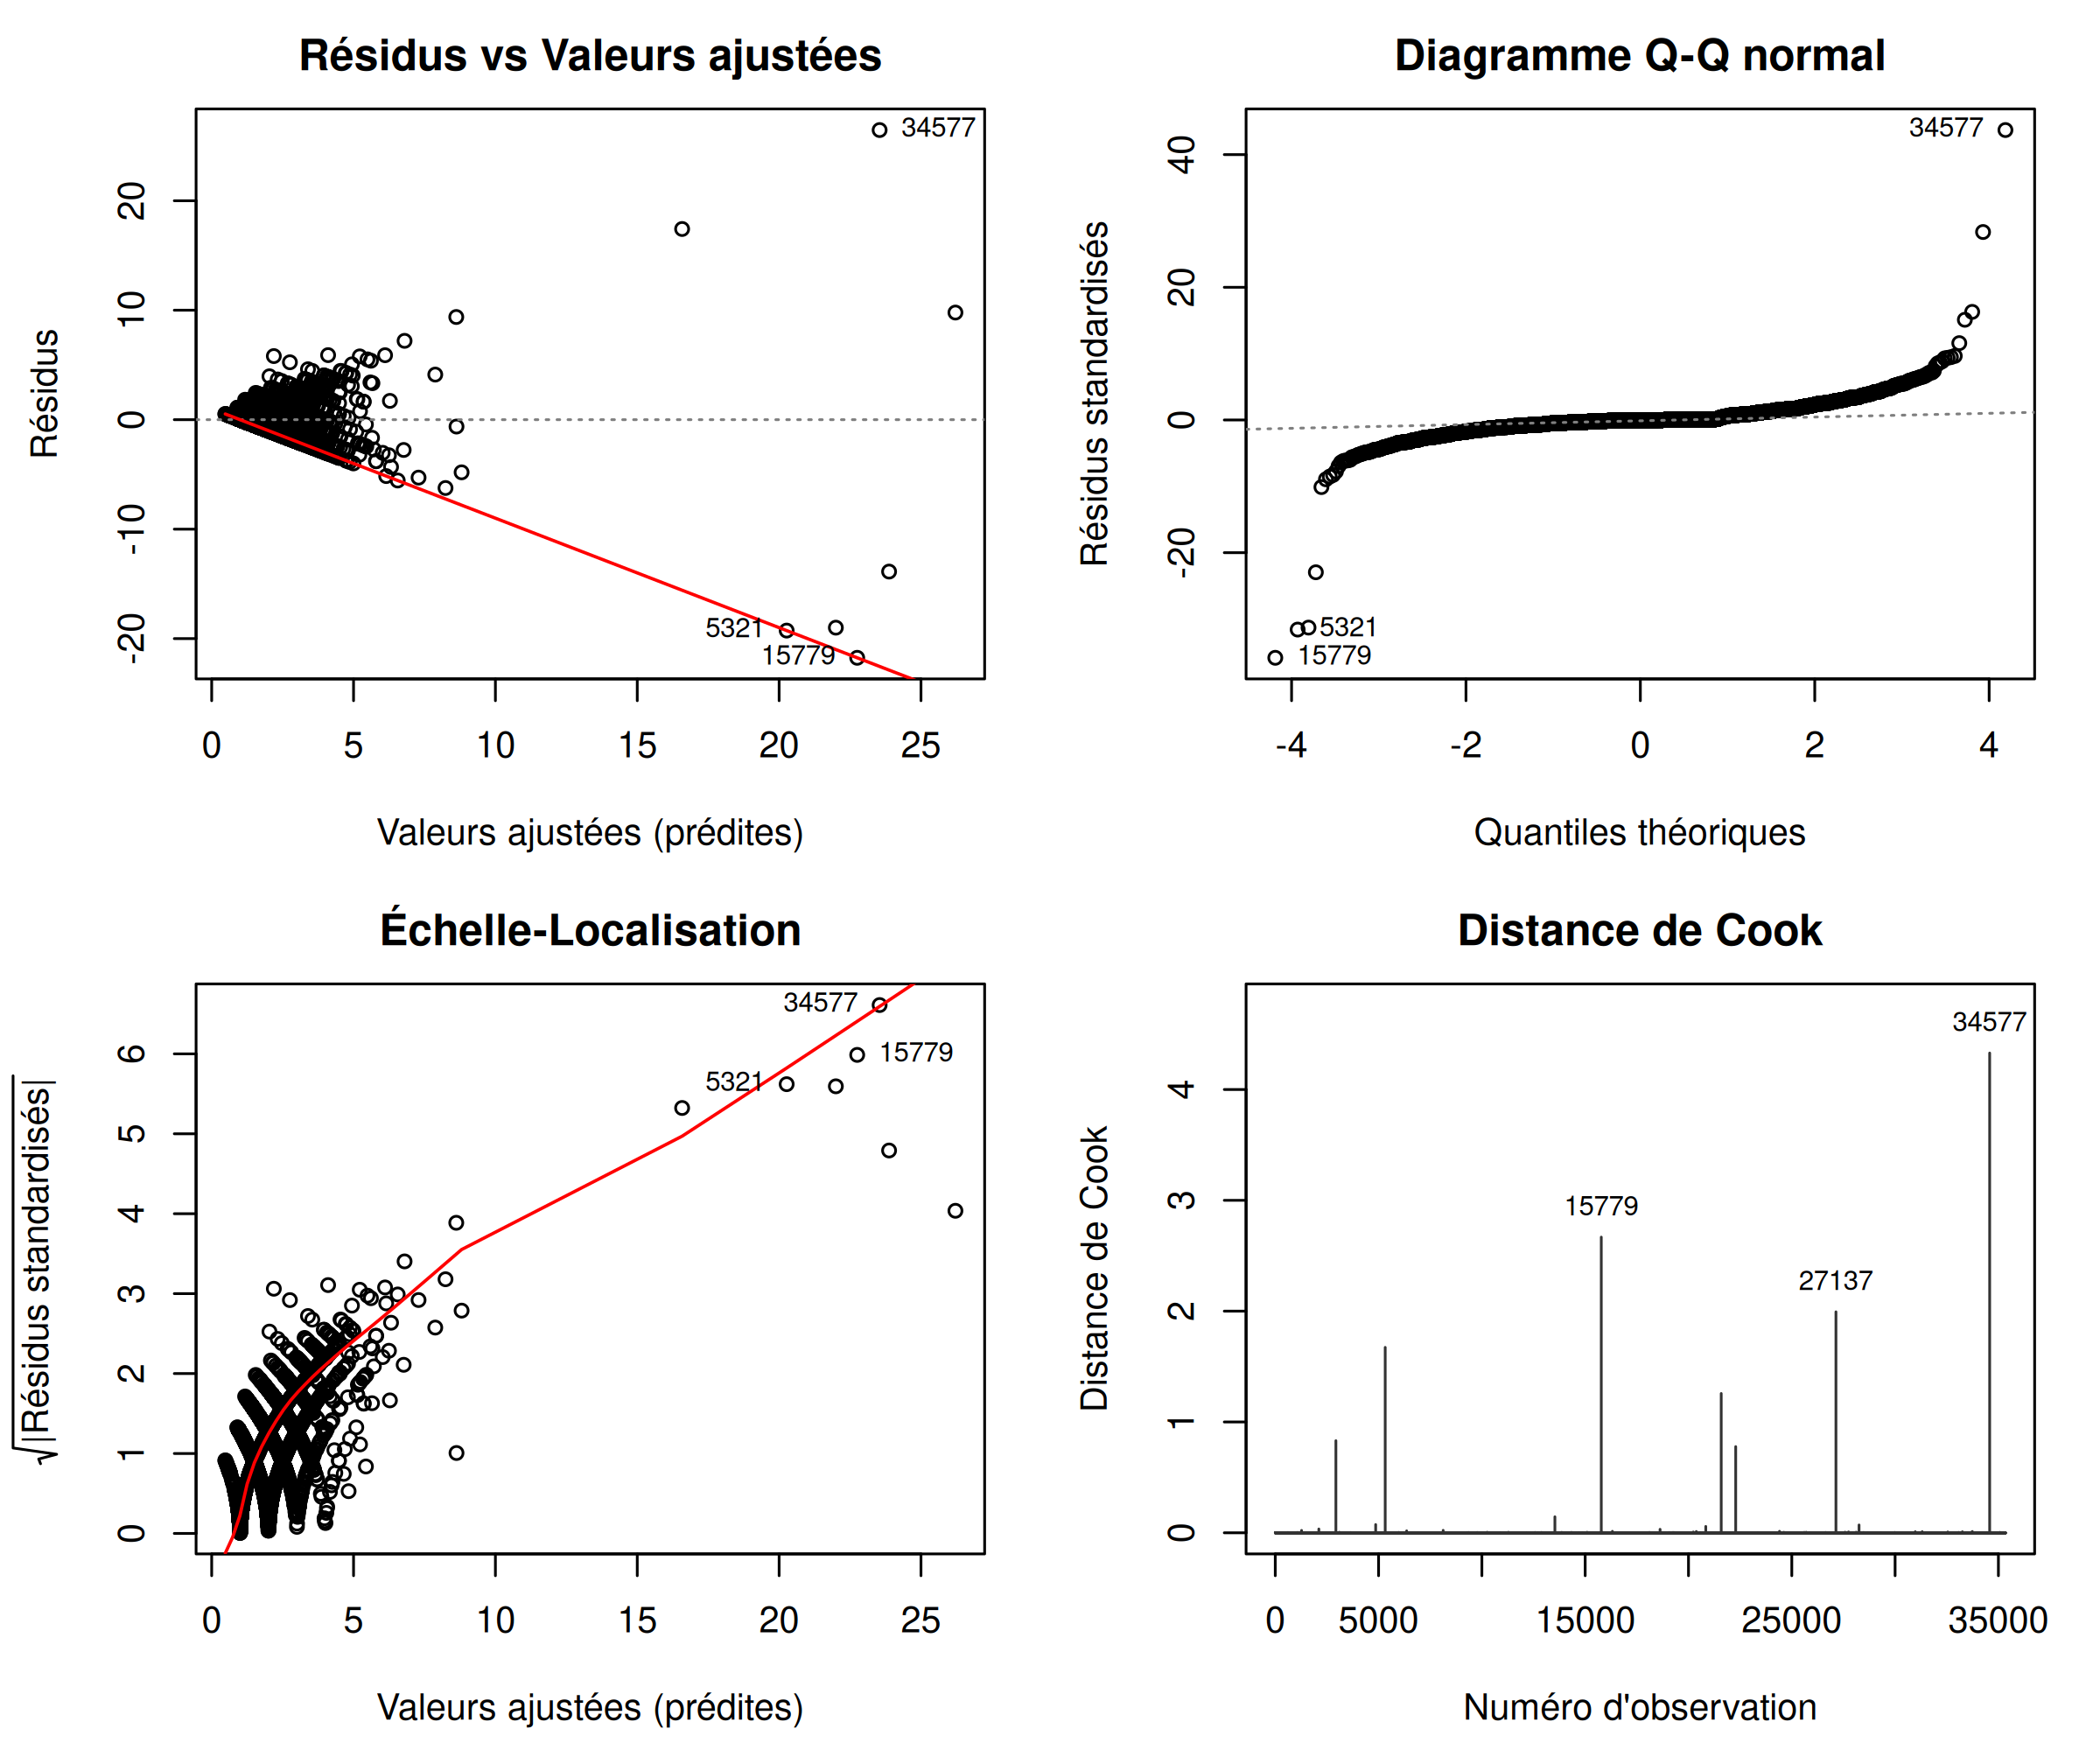
\includegraphics[width=0.85\linewidth]{diag_modele.png}
\caption{Diagnostic du modèle final : résidus en fonction des valeurs ajustées (haut gauche), diagramme Q-Q normal (haut droite), échelle--localisation (bas gauche) et distance de Cook (bas droite).}
\label{fig:diag_modele}
\end{figure}

La variable $Y$ est un comptage entier dont $79\,\%$ des valeurs valent 1 : les résidus prennent de nombreuses valeurs identiques, donc le test de Kolmogorov--Smirnov est indicatif. L'écart observé ($D = 0{,}26$) est toutefois très important, et les résidus vont de $-21{,}8$ à $+26{,}5$. Les conditions de normalité et d'homoscédasticité ne sont pas vérifiées. L'indépendance des observations est admise à ce stade, et la dépendance spatiale des résidus est examinée à la section~\ref{sec:spatial}.

\noindent\textit{Observations aberrantes et influentes.} Le seuil de levier $2p/n$ ($1{,}5\times10^{-3}$) est dépassé par $3\,587$ accidents ; un levier n'est préoccupant que s'il est aussi influent. La distance de Cook maximale vaut $4{,}33$ et cinq accidents dépassent le seuil de 1 (tableau~\ref{tab:influents}).

\begin{table}[H]
\centering
\small
\begin{tabular}{cccc}
\toprule
\textbf{Usagers} & \textbf{Victimes} & \textbf{Véhicules} & \textbf{Zone} \\
\midrule
43 & 1  & 1 & hors agglomération \\
49 & 1  & 2 & hors agglomération \\
51 & 10 & 1 & hors agglomération \\
48 & 3  & 2 & en agglomération \\
50 & 50 & 1 & hors agglomération \\
\bottomrule
\end{tabular}
\caption{Accidents dont la distance de Cook dépasse 1 (tous impliquent plus de 40 usagers et un autobus ou un autocar).}
\label{tab:influents}
\end{table}

Ces accidents sont réels (43 à 51 personnes impliquées, très éloignées de la masse des accidents à 1 à 3 personnes) et impliquent tous un autobus ou un autocar. En les retirant de l'échantillon d'apprentissage, aucun coefficient significatif ne change de signe, mais certains varient sensiblement: nombre de véhicules $-0{,}215 \to -0{,}299$, nombre d'usagers $0{,}455 \to 0{,}521$, présence d'un jeune $0{,}040 \to 0{,}022$, pluie forte $-0{,}052 \to -0{,}033$. Le RMSE sur le jeu de test varie à peine ($0{,}6086 \to 0{,}6096$). Ces observations étant réelles et porteuses d'une information physique majeure, nous faisons le choix méthodologique de les conserver.

\subsection{Corrections essayées : transformations de $Y$ et erreurs robustes}
Lorsque les conditions de validité ne sont pas vérifiées, une transformation de la variable cible $Y$ peut être envisagée. Nous avons d'abord recherché la puissance $\lambda$ de la transformation de Box--Cox, $Y^{(\lambda)} = (Y^{\lambda} - 1)/\lambda$ (logarithme si $\lambda = 0$), qui contient la racine carrée ($\lambda = 0{,}5$) et le logarithme comme cas particuliers. Sur l'intervalle testé $[-2\,;\,2]$, la log-vraisemblance est maximale sur la borne gauche ($\lambda = -2$, figure~\ref{fig:boxcox}) et décroît continuellement vers la droite (chutant jusqu'à $-240\,000$ pour $\lambda = 2$). La courbe ne trouve aucun sommet et continue de monter vers la gauche ($\lambda < -2$) : il n'y a donc aucune valeur interprétable parmi les transformations usuelles ($\lambda \in \{0\,;\,0{,}5\,;\,1\}$). Cela s'explique par la forte proportion d'accidents à une seule victime ($79\,\%$), que la transformation cherche à regrouper.


\begin{figure}[H]
\centering
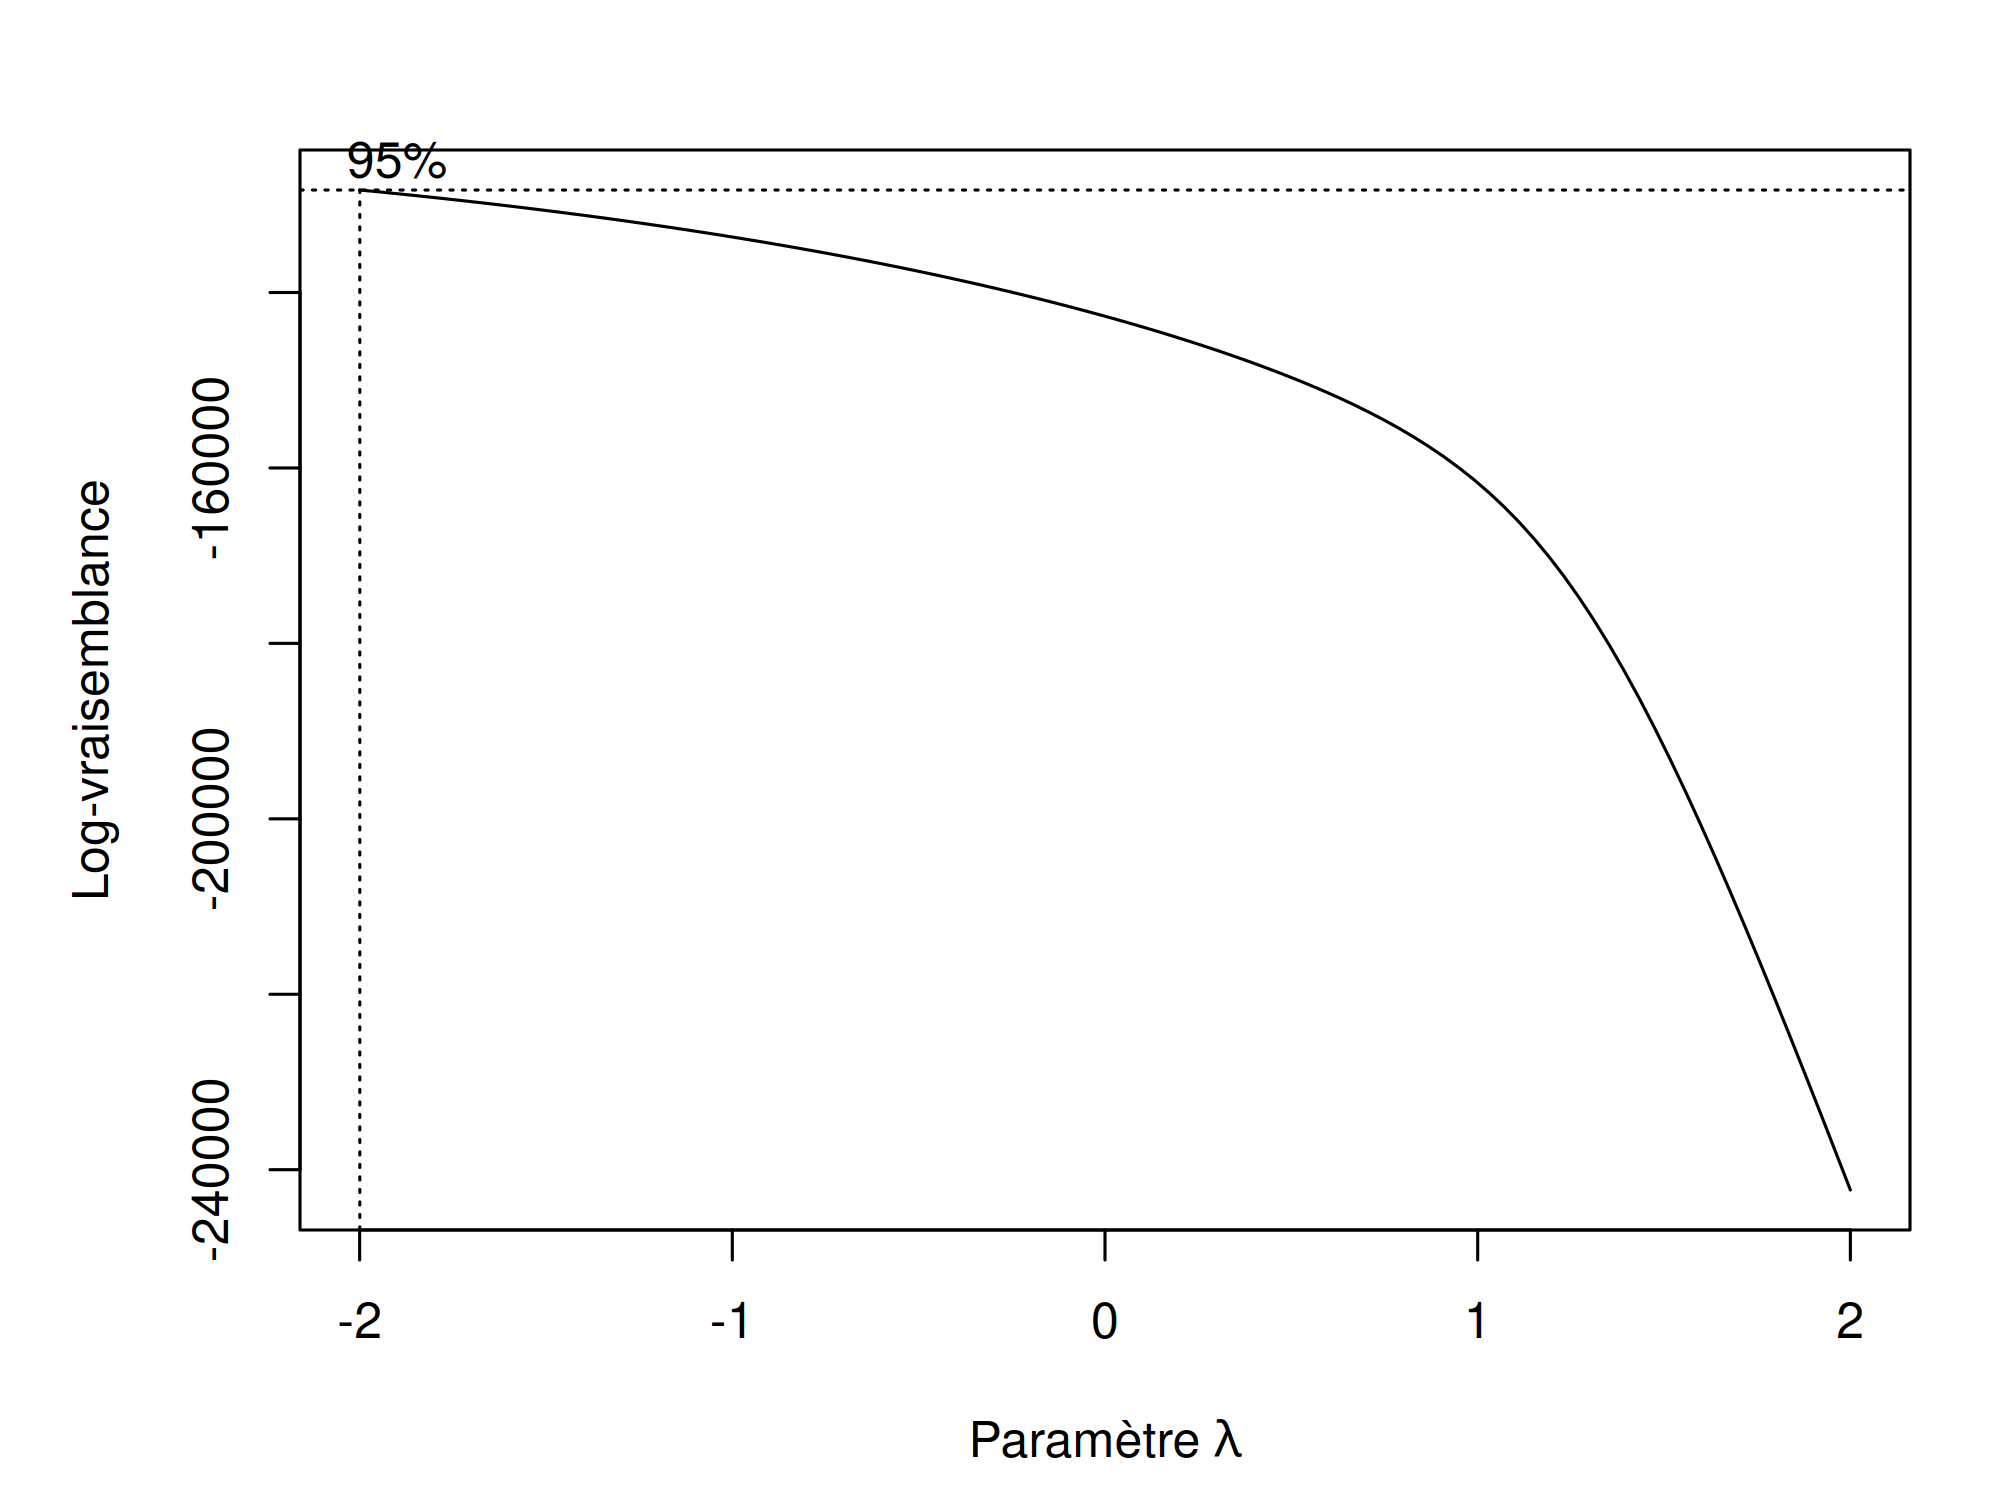
\includegraphics[width=0.55\linewidth]{boxcox.png}
\caption{Vraisemblance profilée de la transformation de Box--Cox : maximum au bord de l'intervalle testé ($\lambda = -2$).}
\label{fig:boxcox}
\end{figure}

Nous avons donc comparé les deux transformations usuelles (racine carrée et logarithme), ajustées avec les mêmes variables.

\begin{table}[H]
\centering
\small
\begin{tabular}{lcccc}
\toprule
\textbf{Modèle} & \textbf{BP} & \textbf{KS ($D$)} & \textbf{RMSE test} & \textbf{MAE test} \\
\midrule
Sans transformation & $12\,958$ & $0{,}260$ & $0{,}6086$ & $0{,}3175$ \\
Racine carrée       & $11\,797$ & $0{,}256$ & $0{,}6700$ & $0{,}3221$ \\
Logarithme          & $14\,521$ & $0{,}260$ & $9{,}87$   & $0{,}4152$ \\
\bottomrule
\end{tabular}
\caption{Comparaison des transformations de $Y$ (RMSE et MAE calculés après rétro-transformation, sur le jeu de test).}
\label{tab:transfo}
\end{table}

Dans tous les cas l'homoscédasticité et la normalité restent rejetées ($p < 2{,}2\times10^{-16}$), la racine carrée ne réduisant que légèrement les statistiques de Breusch--Pagan et de Kolmogorov--Smirnov. Les prédictions sont moins bonnes qu'avec $Y$ non transformée (le RMSE du logarithme est faussé par la fonction exponentielle). Le modèle est donc conservé sur l'échelle d'origine, ce qui garde des coefficients directement interprétables en nombre de victimes.

Pour tenir compte de la variance non constante, les $p$-valeurs sont recalculées avec des erreurs standard robustes (HC3). Cette méthode complète la remédiation proposée qui n'a pas abouti. Les coefficients ne changent pas, seule l'incertitude est réévaluée. Les statistiques $t$ baissent (par exemple, nombre de véhicules : $-16{,}20 \to -2{,}55$), la pluie forte et la collision à trois véhicules ou plus à collisions multiples cessent d'être significatives à 5\,\%, et les autres variables significatives le restent (tableau~\ref{tab:reg_final}).

\subsection{Performance sur le jeu de test}
\begin{table}[H]
\centering
\small
\begin{tabular}{lcc}
\toprule
\textbf{Modèle} & \textbf{RMSE} & \textbf{MAE} \\
\midrule
Prédiction par la moyenne de l'apprentissage & $0{,}8293$ & $0{,}5092$ \\
Modèle linéaire final (avec \texttt{nb\_usagers}) & $0{,}6086$ & $0{,}3175$ \\
\bottomrule
\end{tabular}
\caption{Erreurs de prédiction sur le jeu de test ($n = 15\,146$), en nombre de victimes.}
\label{tab:perf_test}
\end{table}
Le modèle réduit le RMSE de $27\,\%$ par rapport à la moyenne seule, ce qui correspond à un coefficient de détermination d'environ $0{,}46$ sur le jeu de test (calculé comme $1 - \text{RMSE}^2/\text{RMSE}_{\text{moyenne}}^2$). Ces résultats serviront de référence pour la comparaison avec les modèles de la partie~3, évalués sur ces mêmes accidents.

\subsection{Rôle du nombre d'usagers : analyse de sensibilité}\label{sec:sensibilite}
Les variables \og présence d'un jeune\fg{}, \og présence d'un senior\fg{} ou \og non-port documenté\fg{} valent 1 dès qu'\emph{au moins un} usager correspond : plus il y a de personnes impliquées, plus elles valent souvent 1, et plus il peut y avoir de victimes. Elles captent donc en partie la taille de l'accident. Le tableau~\ref{tab:sensibilite} compare les modèles complets sans, puis avec \texttt{nb\_usagers}.

\begin{table}[H]
\centering
\small
\begin{tabular}{lcc}
\toprule
\textbf{Coefficient} & \textbf{Sans \texttt{nb\_usagers}} & \textbf{Avec \texttt{nb\_usagers}} \\
\midrule
Été (référence : hiver)               & $+0{,}053$ & $+0{,}008$ \\
Présence d'un jeune (18--24 ans)      & $+0{,}189$ & $+0{,}038$ \\
Présence d'un senior (65 ans et plus) & $+0{,}058$ & $-0{,}004$ \\
Non-port documenté ceinture / casque  & $+0{,}316$ & $+0{,}149$ \\
Nombre de véhicules                   & $+0{,}364$ & $-0{,}214$ \\
\midrule
RMSE sur le jeu de test               & $0{,}7586$ & $0{,}6088$ \\
\bottomrule
\end{tabular}
\caption{Coefficients du modèle complet sans et avec le nombre d'usagers.}
\label{tab:sensibilite}
\end{table}

L'effet apparent de l'été, des jeunes ou des seniors s'estompe fortement dès que le nombre de personnes est pris en compte : sans ce contrôle, ces variables se lisent surtout comme des indicateurs de la taille de l'accident. Le gain de prédiction (RMSE de $0{,}76$ à $0{,}61$) vient en grande partie de ce lien quasi mécanique entre la cible et \texttt{nb\_usagers}.

\subsection{Test direct de la saison et de la météo}\label{sec:test_direct}
La saison (4 modalités, soit 3 coefficients par rapport à l'hiver pris en référence) et la météo (9 modalités, soit 8 coefficients par rapport à la météo normale) comportent plusieurs modalités : nous testons chaque variable d'un seul coup dans le modèle complet. Le test de Fisher suppose une variance constante, ce qui n'est pas le cas ; nous le complétons par un test de Wald avec la matrice de variance robuste HC3. Le test de Wald avec matrice de variance robuste (HC3), tout comme le test $F$ par variable (\texttt{drop1}), prolonge le test de significativité globale du modèle à un groupe de coefficients, et la variance robuste répond à la violation de l'homoscédasticité constatée à la section~\ref{sec:conditions}. Hypothèses : $H_0$ : tous les coefficients de la variable sont nuls ; $H_1$ : au moins un est non nul.

\begin{table}[H]
\centering
\small
\begin{tabular}{lcccccc}
\toprule
\textbf{Variable} & \textbf{ddl} & \textbf{$F$} & \textbf{$p$ (Fisher)} & \textbf{$\chi^2$ (Wald, HC3)} & \textbf{$p$ (Wald, HC3)} \\
\midrule
Saison                       & 3 & $0{,}49$ & $0{,}689$ & $1{,}30$  & $0{,}730$ \\
Conditions météo             & 8 & $2{,}65$ & $0{,}007$ & $16{,}08$ & $0{,}041$ \\
Luminosité                   & 4 & $1{,}15$ & $0{,}331$ & $3{,}27$  & $0{,}514$ \\
Vitesse maximale autorisée   & 1 & $2{,}03$ & $0{,}154$ & $0{,}68$  & $0{,}411$ \\
Présence d'un senior         & 1 & $0{,}27$ & $0{,}602$ & $0{,}22$  & $0{,}642$ \\
\bottomrule
\end{tabular}
\caption{Tests des variables retirées par la sélection, ou étudiées dans la problématique, dans le modèle complet.}
\label{tab:drop1}
\end{table}

À nombre de personnes impliquées et à types de véhicules donnés, aucun effet de la saison n'est détecté. Pour la météo, l'association est faible mais détectée : $p = 0{,}041$ avec le test robuste, $p = 0{,}007$ avec le test de Fisher. Elle vient surtout de la pluie légère ($-0{,}023$ victime), de la neige ou de la grêle ($-0{,}134$) et de la pluie forte ($-0{,}052$) : ces accidents comptent un peu moins de victimes en moyenne, soit de 2 à 13 victimes de moins pour 100 accidents. Ce signe négatif, a priori contre-intuitif, pourrait refléter une adaptation comportementale des conducteurs (vigilance accrue et vitesses réduites sous les intempéries) ; en l'absence de mesure de la vitesse réelle au moment de l'impact dans la base, nous nous limitons à constater cette association sans affirmer de causalité.

Ce résultat est à prendre avec prudence. Il est proche du seuil de 5\,\%, il porte sur huit modalités testées à la fois, et il dépend de la spécification : dans une première version du modèle sans les types de véhicules, le test de Fisher donnait $p = 0{,}097$ et la météo n'était pas retenue par la sélection. Dans tous les cas, ces accidents ne présentent pas plus de victimes que les accidents par météo normale.

\subsection{Limites}
\begin{itemize}
    \item Les résidus ne sont ni normaux ni de variance constante, et les transformations usuelles n'améliorent pas la situation : seules les $p$-valeurs corrigées (HC3) sont utilisées, et aucun intervalle de prédiction n'est présenté.
    \item La cible est un comptage, dont $79\,\%$ des valeurs valent 1 ; l'estimation d'un modèle adapté aux données de comptage (Poisson, binomiale négative) constituerait un prolongement naturel.
    \item Une grande partie du pouvoir prédictif provient de \texttt{nb\_usagers}, lié mécaniquement à la cible.
    \item Le résultat sur la météo est faible, proche du seuil de 5\,\% et sensible à l'ajout des types de véhicules ; la sélection de variables ne garantit pas que d'autres variables non testées ne le modifieraient pas.
    \item L'unité d'analyse étant l'accident ($n = 50\,486$) et non l'usager, les variables comportementales et démographiques sont des indicatrices de présence (\og au moins un usager ou véhicule concerné\fg{}) : elles mesurent l'impact d'un facteur de risque sur le bilan global de l'accident sans isoler la gravité propre subie par chaque individu. De plus, la valeur 0 de la variable de non-port signifie \og aucun non-port documenté\fg{}, et non pas \og tous équipés\fg{} (l'équipement n'est pas évaluable pour $6\,998$ accidents).
    \item Les résultats décrivent des associations observées sur les accidents corporels de 2024 : ils ne permettent pas de conclure à des relations causales.
\end{itemize}
% ==============================================================================
% SECTION 5 : ANALYSE SPATIALE
% ==============================================================================
\section{Analyse spatiale}\label{sec:spatial}

La deuxième partie de la problématique demande si le nombre de victimes présente une dépendance spatiale à l'échelle départementale. Pour chaque département, nous calculons le nombre moyen de victimes par accident, le nombre moyen de personnes impliquées par accident et le résidu moyen du modèle linéaire de la section~\ref{sec:conditions} (écart entre le nombre observé et le nombre prédit). L'étude porte sur les $N = 94$ départements de la France métropolitaine continentale ; la Corse et l'outre-mer sont exclus car ils n'ont pas de frontière commune avec les autres départements. Les moyennes reposent sur des effectifs très différents (de $61$ à $4\,191$ accidents par département).

\subsection{Voisinage et indices utilisés}
Deux départements sont voisins s'ils partagent une frontière (voisinage de type \emph{queen}), à partir des contours simplifiés des départements issus de l'IGN. Le réseau compte $474$ liens, soit $5{,}04$ voisins par département en moyenne. La matrice de poids $W = (w_{ij})$ est standardisée par ligne : chaque ligne somme à 1.

L'indice de Moran évalue l'autocorrélation globale (covariance des écarts à la moyenne), tandis que le coefficient de Geary privilégie les contrastes locaux par les écarts directs entre voisins $(Z_i - Z_j)^2$. Pour une variable $Z$ mesurée sur $n$ départements, leurs expressions s'écrivent :
\[
I = \frac{n}{\sum_{i \neq j} w_{ij}} \cdot \frac{\sum_{i,j} w_{ij}(Z_i - \bar{Z})(Z_j - \bar{Z})}{\sum_i (Z_i - \bar{Z})^2},
\qquad
C = \frac{n-1}{2\sum_{i \neq j} w_{ij}} \cdot \frac{\sum_{i,j} w_{ij}(Z_i - Z_j)^2}{\sum_i (Z_i - \bar{Z})^2}.
\]
Sans autocorrélation, $I$ vaut environ $\mathbb{E}[I] = -1/(n-1) = -0{,}011$ et $C$ vaut 1. Une valeur de $I$ supérieure à cette espérance, ou de $C$ inférieure à 1, indique que les départements voisins ont des valeurs proches. Pour chaque indice, le test a pour hypothèses
\[
H_0 : \text{absence d'autocorrélation spatiale} \quad \text{contre} \quad H_1 : \text{présence d'autocorrélation spatiale},
\]
et la $p$-valeur est calculée sous l'hypothèse de randomisation (fonctions \texttt{moran.test} et \texttt{geary.test}, test bilatéral).

\subsection{Résultats}
\begin{table}[H]
\centering
\small
\begin{tabular}{lcccc}
\toprule
 & $I$ de Moran & $p$ & $C$ de Geary & $p$ \\
\midrule
Nombre moyen de victimes            & $0{,}235$ & $1{,}7\times10^{-4}$ & $0{,}764$ & $6{,}9\times10^{-4}$ \\
Nombre moyen de personnes impliquées & $0{,}212$ & $4{,}5\times10^{-4}$ & $0{,}798$ & $7{,}7\times10^{-3}$ \\
Résidu moyen du modèle linéaire      & $0{,}013$ & $0{,}72$             & $0{,}968$ & $0{,}64$ \\
\bottomrule
\end{tabular}
\caption{Autocorrélation spatiale départementale (voisinage par frontières communes, $N = 94$).}
\label{tab:moran_contig}
\end{table}

Le nombre moyen de victimes et le nombre moyen de personnes impliquées présentent une autocorrélation spatiale positive : les départements voisins se ressemblent. Pour le résidu moyen du modèle, aucune autocorrélation n'est détectée.

Pour vérifier que ces conclusions ne dépendent pas de la définition du voisinage, nous les avons recalculées en prenant pour voisins les $k$ départements les plus proches ($k = 3, 5, 8$), les distances étant mesurées entre les points moyens des accidents de chaque département.

\begin{table}[H]
\centering
\small
\begin{tabular}{ccccccc}
\toprule
 & \multicolumn{4}{c}{Nombre moyen de victimes} & \multicolumn{2}{c}{Résidu moyen} \\
\cmidrule(lr){2-5}\cmidrule(lr){6-7}
$k$ & $I$ & $p$ & $C$ & $p$ & $I$ & $p$ \\
\midrule
3 & $0{,}250$ & $6{,}1\times10^{-4}$ & $0{,}774$ & $7{,}3\times10^{-3}$ & $-0{,}044$ & $0{,}66$ \\
5 & $0{,}157$ & $4{,}9\times10^{-3}$ & $0{,}873$ & $0{,}050$            & $-0{,}002$ & $0{,}89$ \\
8 & $0{,}104$ & $0{,}013$            & $0{,}913$ & $0{,}111$            & $0{,}008$  & $0{,}69$ \\
\bottomrule
\end{tabular}
\caption{Sensibilité au choix du nombre de voisins ($k$ plus proches voisins).}
\label{tab:moran_knn}
\end{table}

Le $I$ de Moran reste positif et significatif pour les trois valeurs de $k$, et diminue quand le voisinage s'élargit ($0{,}25$, $0{,}16$, $0{,}10$) : la ressemblance concerne surtout les voisins proches. Le $C$ de Geary va dans le même sens mais n'est plus significatif pour $k = 8$.

\subsection{Cartes}
\begin{figure}[H]
\centering
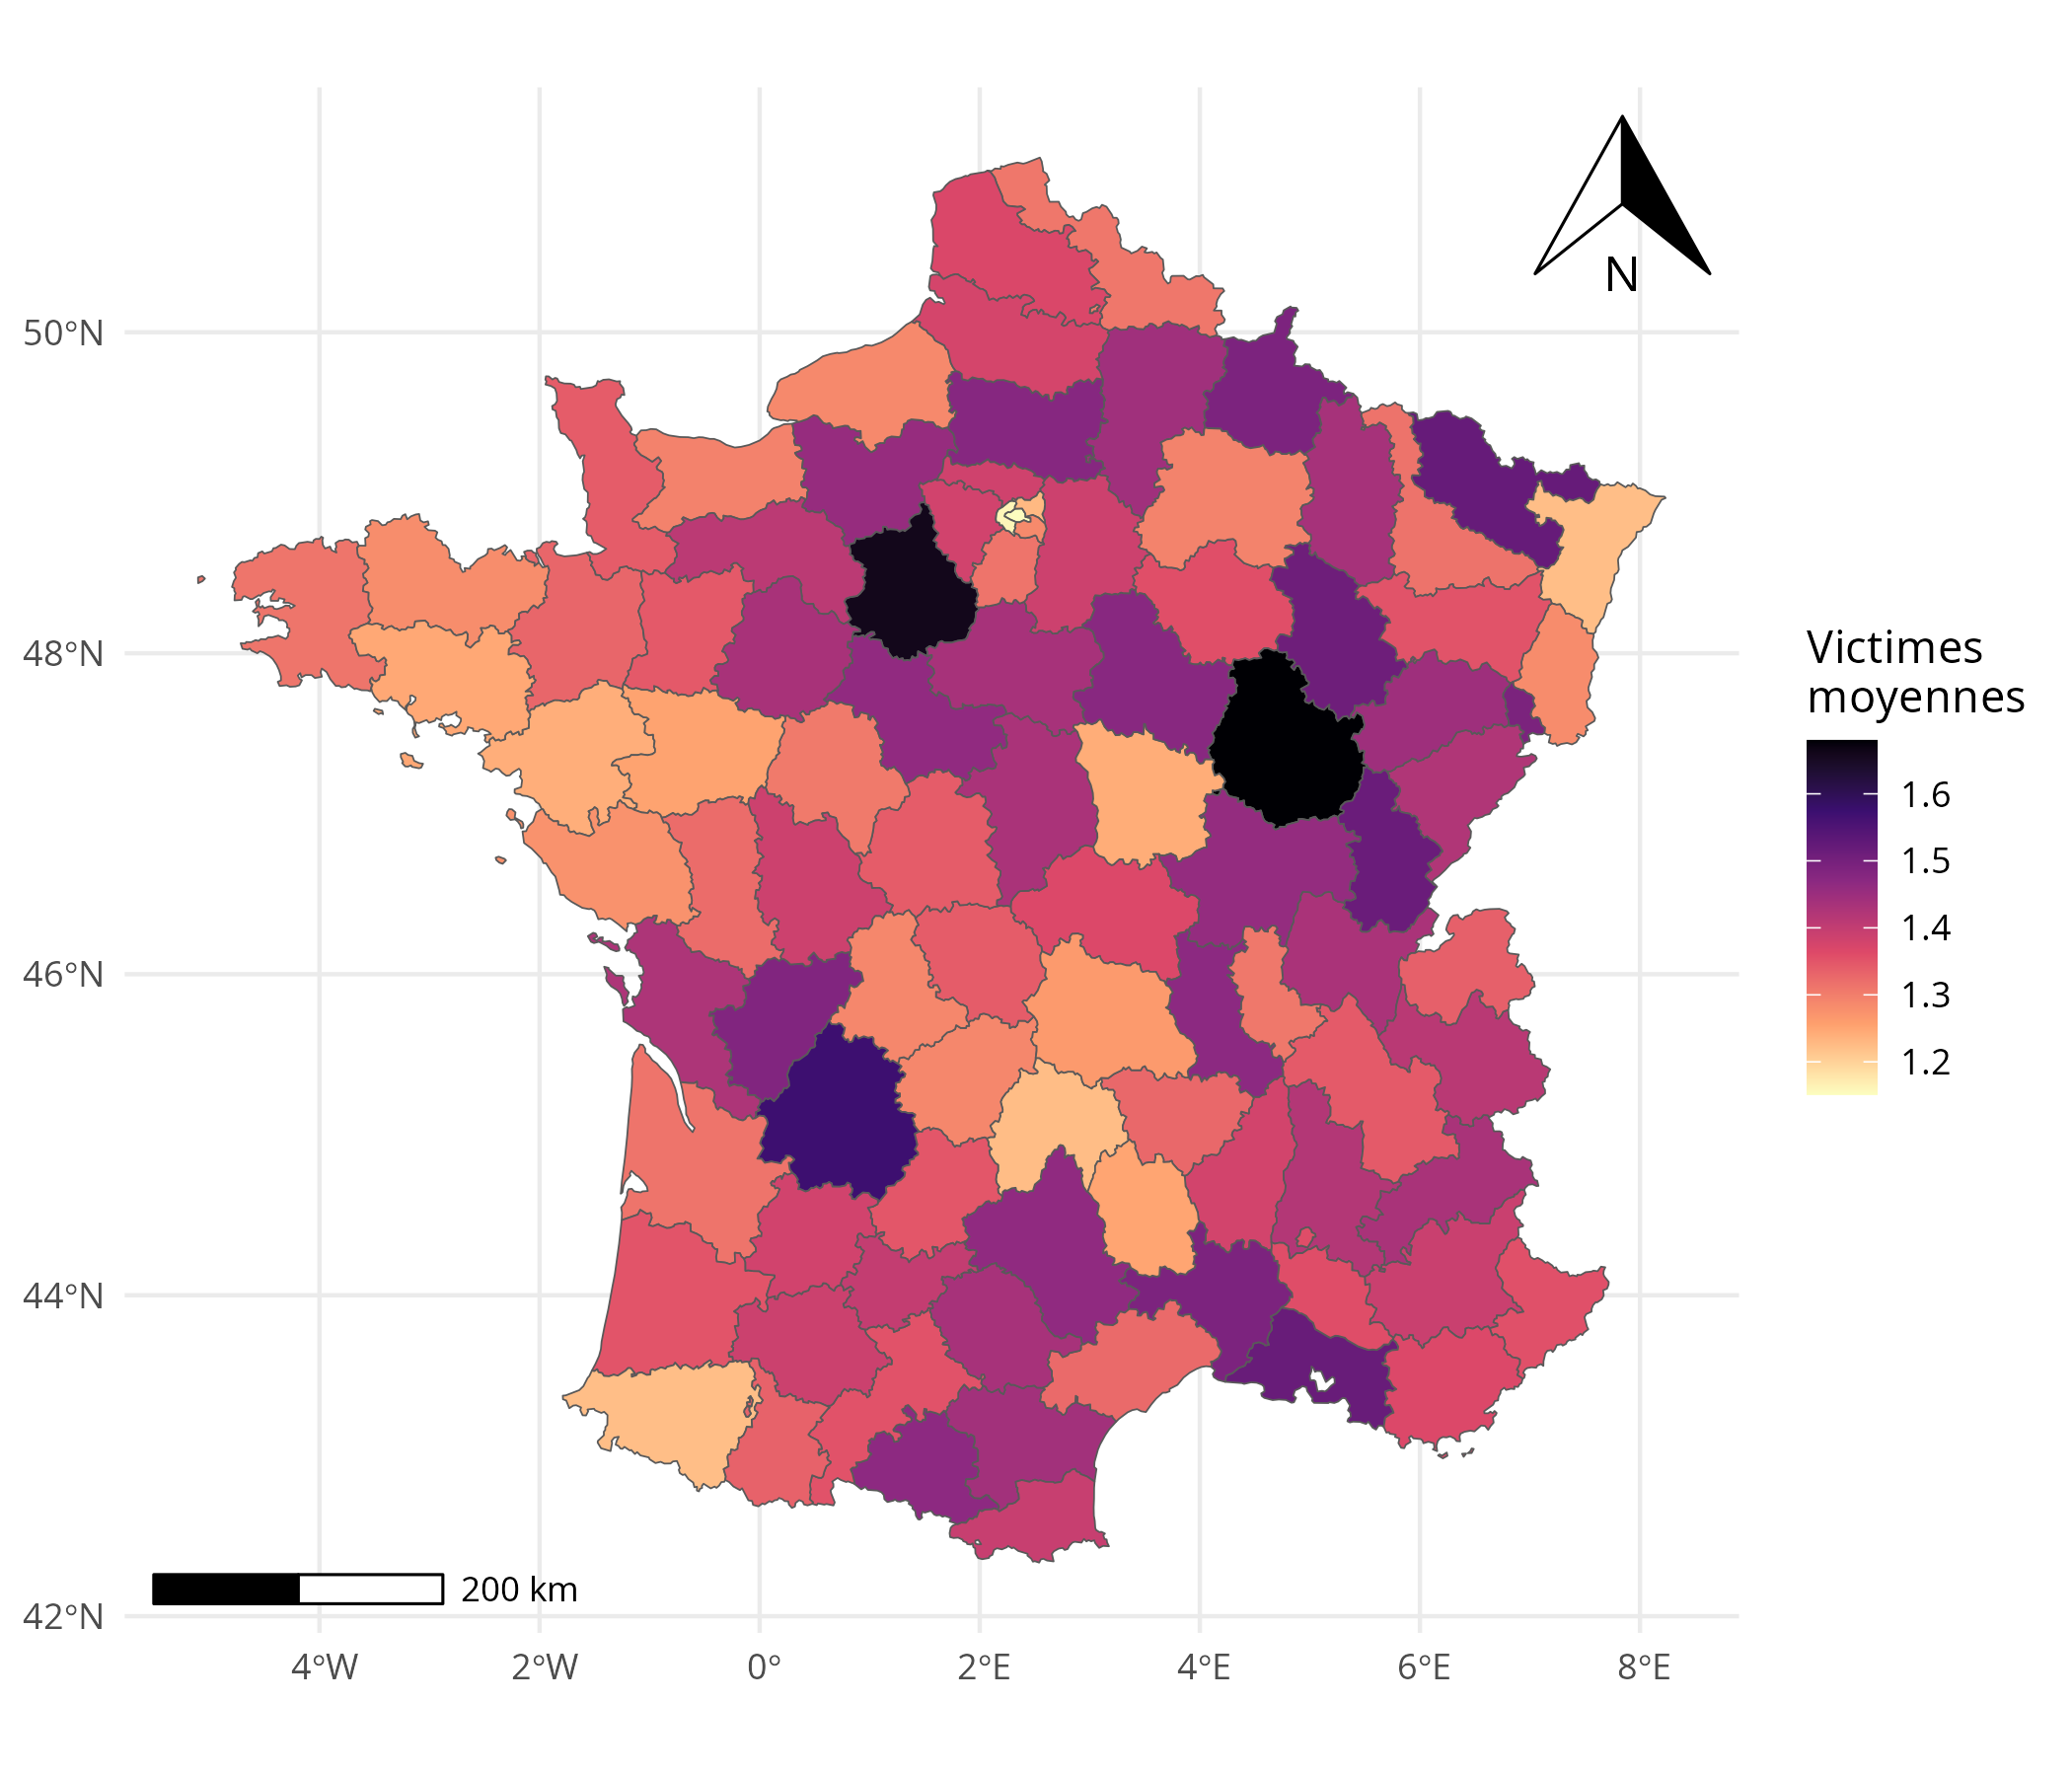
\includegraphics[width=0.6\linewidth]{carte_victimes.png}
\caption{Nombre moyen de victimes par accident et par département (échelle indicative).}
\label{fig:carte_victimes}
\end{figure}

\begin{figure}[H]
\centering
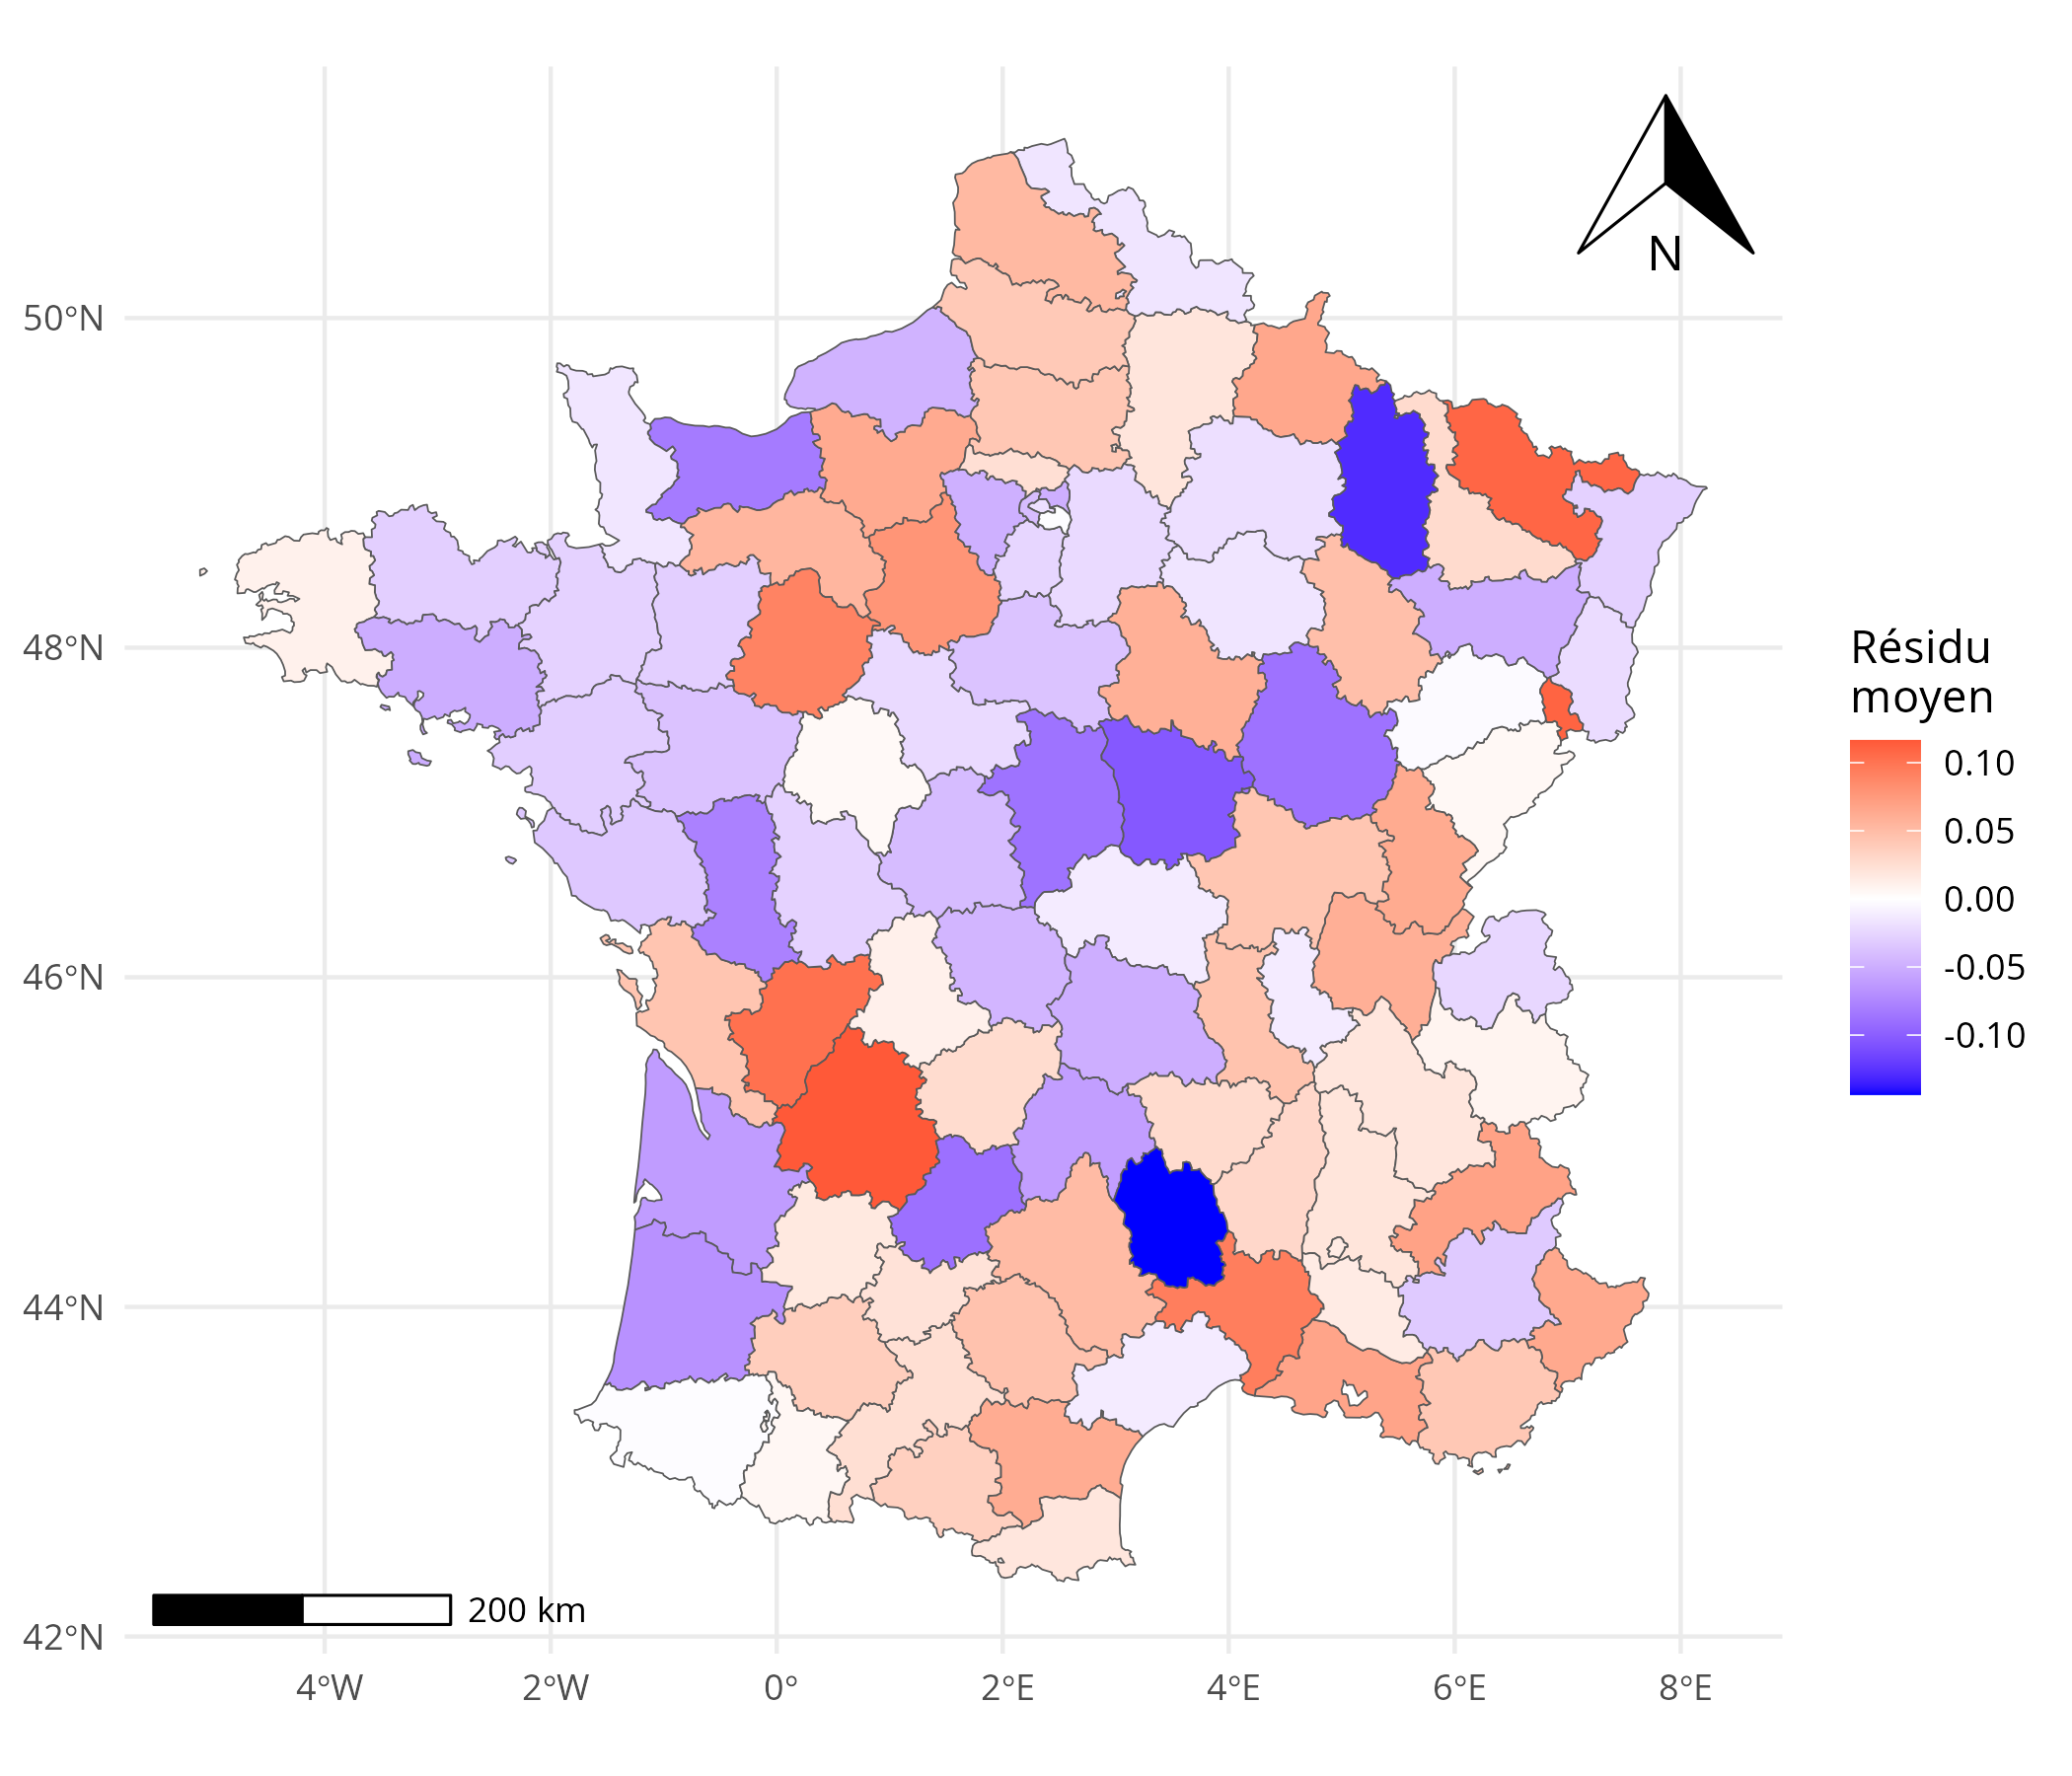
\includegraphics[width=0.6\linewidth]{carte_residus.png}
\caption{Résidu moyen du modèle linéaire par département (blanc : le modèle ne se trompe pas en moyenne).}
\label{fig:carte_residus}
\end{figure}

La carte des victimes ne fait apparaître ni couloir rhodanien ni bloc méditerranéen. Les valeurs les plus élevées sont observées en Côte-d'Or ($1{,}68$ ; $206$ accidents), en Eure-et-Loir ($1{,}66$ ; $262$), en Dordogne ($1{,}57$ ; $175$), en Moselle ($1{,}52$ ; $329$) et dans les Bouches-du-Rhône ($1{,}52$ ; $2\,120$). Les plus basses sont celles de Paris ($1{,}15$ ; $4\,191$), des Hauts-de-Seine ($1{,}16$ ; $2\,485$), du Bas-Rhin, des Pyrénées-Atlantiques et du Cantal ($1{,}22$ chacun). Les départements aux moyennes élevées ont souvent peu d'accidents : une moyenne calculée sur 200 accidents est plus instable qu'une moyenne sur 4\,000, et un seul accident à plus de 40 personnes suffit à la déplacer sensiblement. De son côté, la carte des résidus ne fait pas apparaître de structure nette : quelques groupes de départements de même signe se devinent (centre et ouest plutôt négatifs, nord et sud-est plutôt positifs), mais des départements voisins ont aussi des signes opposés (la Meuse et la Moselle, la Lozère et le Gard). Les valeurs les plus extrêmes concernent des départements à faibles effectifs (Lozère : $72$ accidents, Meuse : $117$). Cela correspond à l'absence d'autocorrélation du tableau~\ref{tab:moran_contig}.

\subsection{Conclusion et limites}
Le nombre moyen de victimes par accident présente une autocorrélation spatiale positive modérée ($I = 0{,}235$, $p = 1{,}7\times10^{-4}$), de même que le nombre moyen de personnes impliquées. Une fois le modèle linéaire appliqué (nombre de personnes, types de véhicules et autres variables pris en compte), les résidus ne présentent plus d'autocorrélation détectable ($I = 0{,}013$, $p = 0{,}72$) : la ressemblance entre départements voisins est cohérente avec une structure spatiale du nombre de personnes impliquées par accident et de la composition du parc de véhicules impliqués, sans que nous cherchions à l'expliquer.
\begin{itemize}
    \item Avec seulement $94$ départements, une dépendance faible peut ne pas être détectée : l'absence de significativité sur les résidus n'est pas une preuve d'indépendance.
    \item Le résultat varie avec le voisinage (par exemple, le $C$ de Geary n'est plus significatif pour $k = 8$).
    \item Les points utilisés pour les $k$ plus proches voisins sont des moyennes de positions d'accidents, pas les centres géométriques des départements.
    \item Les résidus sont calculés sur tous les accidents, apprentissage et test confondus.
    \item Une structure spatiale ne dit rien sur ses causes.
\end{itemize}


% ==============================================================================
% SECTION 7 : CONCLUSION
% ==============================================================================
\section{Conclusion}

Réponse à la problématique, à partir des $50\,486$ accidents corporels de 2024 en France métropolitaine continentale.
\begin{enumerate}
    \item Saison : sans tenir compte du nombre de personnes impliquées, l'été a la moyenne la plus élevée ($1{,}35$ victime par accident contre $1{,}31$ à $1{,}33$), mais l'écart est faible. À nombre de personnes impliquées et à types de véhicules donnés, plus aucun effet saisonnier n'est détecté (test de Wald robuste, $p = 0{,}73$).
    \item Météo : à nombre de personnes impliquées et à types de véhicules donnés, l'association est faible mais détectée (test de Wald robuste, $p = 0{,}041$). La pluie légère, la neige ou la grêle et la pluie forte sont associées à un peu moins de victimes que la météo normale (de $0{,}02$ à $0{,}13$ victime par accident). Ce résultat est proche du seuil de 5\,\% et dépend de la spécification : sans les types de véhicules, il n'était pas détecté. Il ne permet pas de conclure à une relation causale.
    \item Dépendance spatiale : le nombre moyen de victimes par accident est positivement autocorrélé entre départements voisins ($I = 0{,}235$, $p = 1{,}7\times10^{-4}$), de même que le nombre moyen de personnes impliquées. Les résidus du modèle ne présentent plus d'autocorrélation détectable ($I = 0{,}013$, $p = 0{,}72$).
    \item Prédiction : le modèle linéaire final réduit le RMSE de $27\,\%$ sur le jeu de test par rapport à la moyenne seule ($0{,}609$ contre $0{,}829$ victime), en grande partie grâce au nombre de personnes impliquées. Les facteurs associés à un nombre plus élevé de victimes, à nombre de personnes égal, sont le type de collision (surtout les chocs frontaux), la localisation hors agglomération, le choc contre un obstacle fixe et le non-port documenté de ceinture ou de casque. Ce sont des associations, non des causes.
\end{enumerate}

Les conditions du modèle linéaire (normalité et variance constante des résidus) ne sont pas vérifiées et les transformations usuelles ne les corrigent pas : seuls les tests avec erreurs robustes sont utilisés. Les limites de chaque partie sont détaillées aux sections~4 et~5.

% À compléter après la partie 3 : comparaison avec les modèles de machine learning
% sur le même jeu de test (RMSE du modèle linéaire : 0,6086).

\end{document}